% \documentclass[a4paper,10pt]{article}
\documentclass[review]{siamart}
\usepackage{url}
\usepackage{amssymb}
\usepackage{amsmath}
\usepackage{mathtools}
\usepackage{bm}
\usepackage{stmaryrd}
\usepackage{array}
\usepackage{booktabs}
\usepackage{makecell}
\usepackage{multirow}
\usepackage{empheq}
\usepackage{enumitem}
	\setlist{nosep} % or \setlist{noitemsep} to leave space around whole list
\usepackage{color}
\usepackage{verbatim}
% \usepackage{showlabels}
\usepackage{adjustbox}
\usepackage{hyperref}
\definecolor{darkgreen}{rgb}{0.0, 0.5, 0}
\usepackage[numbers,sort]{natbib}
\usepackage{cleveref}
\usepackage[belowskip=-5pt]{subcaption}
\usepackage{pbox}


\newsiamremark{remark}{Remark}
\newsiamremark{assumption}{Assumption}
\crefname{assumption}{Assumption}{Assumptions}

% \newtheorem{lemma}{Lemma}
% \newtheorem{definition}{Definition}
% \newtheorem{theorem}{Theorem}
% \newtheorem{corollary}{Corollary}

\newcommand{\tcb}{\textcolor{blue}}
\newcommand{\tcp}{\textcolor{purple}}
\newcommand{\todo}[1]{\textcolor{red}{[TODO\@: #1]}}

\newcommand{\OK}[1]{\textcolor{blue}{[OK: #1]}}
\newcommand{\WP}[1]{\textcolor{green}{[WP: #1]}}

\newcommand{\mdet}{\operatorname{det}}
\newcommand{\madj}{\operatorname{adj}}
\DeclareMathOperator{\cL}{\widehat{\mathcal{L}}}
\DeclareMathOperator{\cLs}{\widehat{\mathcal{L}}^2}

% ------------------------------------------------------------------------------------ %
% ------------------------------------------------------------------------------------ %

\newcommand{\TheTitle}{Fast parallel solution of fully implicit Runge-Kutta and discontinuous
	Galerkin in time for numerical PDEs, Part II: nonlinearities and DAEs}
\newcommand{\TheAuthors}{B.S. Southworth, O.A. Krzysik, and W. Pazner}
\headers{Parallel solution of fully implicit Runge-Kutta and DG in time II}{\TheAuthors}
\title{{\TheTitle}\thanks{BSS was supported by Lawrence Livermore National
      Laboratory under contract B639443, and as a Nicholas C. Metropolis Fellow
      under the Laboratory Directed Research and Development program of Los
      Alamos National Laboratory.
  }}

\author{Ben S. Southworth\thanks{Theoretical Division, Los Alamos National Laboratory,
    U.S.A. (\url{southworth@lanl.gov}),
    \url{http://orcid.org/0000-0002-0283-4928}}
    \and
    Oliver A. Krzysik\thanks{School of Mathematics, Monash University,
  	Australia (\url{oliver.krzysik@monash.edu}),
  	\url{https://orcid.org/0000-0001-7880-6512}}
  	\and
  	Will Pazner\thanks{Center for Applied Scientific Computing,
  	Lawrence Livermore National Laboratory,
    U.S.A. (\url{pazner1@llnl.gov})}
}

\ifpdf%
\hypersetup{%
  pdftitle={\TheTitle},
  pdfauthor={\TheAuthors}
}
\fi

% ------------------------------------------------------------------------------------ %
% ------------------------------------------------------------------------------------ %

\begin{document}
\maketitle
\allowdisplaybreaks

\begin{abstract}
Fully implicit Runge-Kutta (IRK) methods have many desirable properties as time
integration schemes in terms of accuracy and stability, but are rarely used in
practice with numerical PDEs due to the difficulty of solving the stage equations.
This paper introduces a theoretical and algorithmic framework for the fast,
parallel solution of the nonlinear equations that arise from
IRK methods applied to nonlinear numerical PDEs, including PDEs with algebraic
constraints. This framework also naturally applies to discontinuous
Galerkin discretizations in time. Moreover, the new method only requires
preconditioners as would be used for backward Euler-type time stepping schemes.
Several new linearizations of the nonlinear IRK equations are developed,
offering faster and more robust convergence than the often-considered simplified
Newton, as well as an effective preconditioner for the true Jacobian if exact
Newton iterations are desired. Inverting these linearizations requires solving a
set of block $2\times 2$ systems. Under quite general assumptions on the
spatial discretization, it is proven that the preconditioned operator has a
condition number of $\sim\mathcal{O}(1)$, with only weak dependence on the
number of stages or integration accuracy. The new
methods are applied to multiple examples of the compressible Euler and Navier
Stokes equations, and the incompressible Euler and Navier Stokes equations
in the vorticity-streamfunction formulation. Up to 10th order accuracy is
demonstrated using Gauss integration, while in all cases 4th-order Gauss integration
requires roughly half the number of preconditioner applications as required
by standard SDIRK methods.
\end{abstract}


% ------------------------------------------------------------------------------------- %
% ------------------------------------------------------------------------------------- %
% ------------------------------------------------------------------------------------- %
\section{Introduction}\label{sec:intro}

% ------------------------------------------------------------------------------------- %
% ------------------------------------------------------------------------------------- %
\subsection{Fully implicit Runge-Kutta}\label{sec:intro:irk}

Consider the method-of-lines approach to the numerical solution of partial differential
equations (PDEs), where we discretize in space and arrive at a system of ordinary
differential equations (ODEs) in time,
%
\begin{align}\label{eq:problem}
	M\mathbf{u}'(t) =  \mathcal{N}(\mathbf{u},t) \quad\text{in }(0,T], \quad \mathbf{u}(0) = \mathbf{u}_0,
\end{align}
%
where $M$ is a mass matrix and $\mathcal{N}:\mathbb{R}^{N} \times \mathbb{R}_+
\mapsto\mathbb{R}^{N}$ is a discrete, time-dependent, nonlinear operator
depending on $t$ and $\mathbf{u}$ (including potential forcing terms). Note,
PDEs with an algebraic constraint, for example, the divergence-free constraint
in Navier Stokes, instead yield a system of differential algebraic equations
(DAEs). DAEs require separate treatment and are addressed in \Cref{sec:dae}.
Now, consider time propagation of \eqref{eq:problem} using an $s$-stage
Runge-Kutta scheme, characterized by the Butcher tableaux
%
\begin{align*}
	\renewcommand\arraystretch{1.2}
	\begin{array}
	{c|c}
	\mathbf{c}_0 & A_0\\
	\hline
	& \mathbf{b}_0^T
	\end{array},
\end{align*}
%
with Runge-Kutta matrix $A_0 = (a_{ij})$, weight vector $\mathbf{b}_0^T = (b_1, \ldots, b_s)^T$,
and quadrature nodes $\mathbf{c}_0 = (c_1, \ldots, c_s)$.

Runge-Kutta methods update the solution using a sum over stage vectors,
%
\begin{align}\label{eq:update}
\mathbf{u}_{n+1} & = \mathbf{u}_n + \delta t \sum_{i=1}^s b_i\mathbf{k}_i,
	\hspace{5ex}\textnormal{where}\\
M\mathbf{k}_i & = \mathcal{N}\left(\mathbf{u}_n + \delta t\sum_{j=1}^s a_{ij}\mathbf{k}_j, t_n+\delta tc_i\right).\label{eq:stages}
\end{align}
%
For nonlinear PDEs, $\mathcal{N}$ is linearized using, for example, a Newton or a
Picard linearization, and each nonlinear iteration then consists of solving the
linearized system of equations. In most cases, such a linearization
is designed to approximate (or equal) the Jacobian of \eqref{eq:stages}. Applying
a chain rule to \eqref{eq:stages} for the partial
$\partial(M\mathbf{k}_i-\mathcal{N}_i)/\partial\mathbf{k}_j$, we see that
the linearized system should take the form
%
\begin{align}\label{eq:k0}
\left( \begin{bmatrix} M  & & \mathbf{0} \\ & \ddots \\ \mathbf{0} & & M\end{bmatrix}
	- \delta t \begin{bmatrix} a_{11}\mathcal{L}_1 & ... & a_{1s}\mathcal{L}_1 \\
	\vdots & \ddots & \vdots \\ a_{s1}\mathcal{L}_s & ... & a_{ss} \mathcal{L}_s \end{bmatrix} \right)
	\begin{bmatrix} \mathbf{k}_1 \\ \vdots \\ \mathbf{k}_s \end{bmatrix}
& = \begin{bmatrix} \mathbf{f}_1 \\ \vdots \\ \mathbf{f}_s \end{bmatrix},
\end{align}
%
where $\mathcal{L}_i\in\mathbb{R}^{N\times N}$
denotes a linearization of the nonlinear function
corresponding to the $i$th stage vector, $\mathcal{N}_i:= \mathcal{N}\left(\mathbf{u}_n +
\delta t\sum_{j=1}^s a_{ij}\mathbf{k}_j, t_n+\delta tc_i\right)$ (the main
point being that the spatially linearized operators, $\mathcal{L}_i$, should
be fixed for a given block row of the full linearized system, as in \eqref{eq:k0}),
and $\mathbf{f}_i$ corresponds to \eqref{eq:stages} evaluated at
the previous nonlinear iterate for $\{\mathbf{k}_i\}$.
Moving forward, we let $\mathcal{L}$ refer to a general, spatially linearized
operator when the stage index is not relevant.

The difficulty in fully implicit Runge-Kutta methods (which we will denote IRK) lies in
solving the $Ns\times Ns$ block linear system in \eqref{eq:k0}. This paper focuses on the
parallel simulation of numerical PDEs, where $N$ is typically very large
and $\mathcal{L}$ is highly ill-conditioned. In such cases, direct
solution techniques to solve \eqref{eq:k0} are not a viable option, and fast, parallel
iterative methods must be used. However, IRK methods are rarely employed in practice due
to the difficulties of solving \eqref{eq:k0}. Even for relatively simple
parabolic PDEs where $-\mathcal{L}$ is symmetric positive definite (SPD), \eqref{eq:k0}
is a large nonsymmetric matrix with significant block coupling. For nonsymmetric
matrices $\mathcal{L}$ that already have inter-variable coupling resulting from
a system of PDEs, traditional
iterative methods are even less likely to yield acceptable performance in solving
\eqref{eq:k0}.

% ------------------------------------------------------------------------------------- %
% ------------------------------------------------------------------------------------- %
\subsection{Discontinuous Galerkin in time}\label{sec:intro:dg}

For completeness, here we repeat the discussion from the companion paper \cite{irk1}
regarding the relation of Discontinuous Galerkin (DG) discretizations in time to IRK
methods. After linearization, DG discretizations in time give rise to linear
algebraic systems of the form
\begin{equation} \label{eq:dg-in-time}
	\left( \begin{bmatrix}
		\delta_{11} M  & & \delta_{1s} M \\
		& \ddots \\
		\delta_{s1} M & & \delta_{ss} M
	\end{bmatrix}
	- \delta t \begin{bmatrix}
		m_{11}\mathcal{L}_1 & ... & m_{1s}\mathcal{L}_1 \\
		\vdots & \ddots & \vdots \\
		m_{s1}\mathcal{L}_s & ... & m_{ss} \mathcal{L}_s
	\end{bmatrix} \right)
		\begin{bmatrix} \mathbf{u}_1 \\ \vdots \\ \mathbf{u}_s \end{bmatrix}
		= \begin{bmatrix} \mathbf{r}_1 \\ \vdots \\ \mathbf{r}_s \end{bmatrix}.
\end{equation}
The coefficients $m_{ij}$ correspond to a temporal mass matrix, the coefficients
$\delta_{ij}$ correspond to a DG weak derivative with upwind numerical flux, and
the unknowns $\mathbf{u}_i$ are the coefficients of the polynomial expansion of
the approximate solution (for example, see \cite{hn,Akrivis2011,Lasaint1974,Makridakis2006}).
Both of the coefficient matrices $\{m_{ij}\}$ and $\{\delta_{ij}\}$ are
invertible. It can be seen that the algebraic form of the DG in time
discretization is closely related to the implicit Runge-Kutta system
\eqref{eq:k0} and, in fact, \eqref{eq:dg-in-time} can be recast in the form of
\eqref{eq:k0} using the invertibility of the matrix $\{\delta_{ij}\}$. In
particular, the degree-$p$ DG method using $(p+1)$-point
Radau quadrature, which is exact for polynomials of degree $2p$, is equivalent
to the Radau IIA collocation method \cite{Makridakis2006}, which is used for
many of the numerical results in \Cref{sec:numerics}.
Thus, although the remainder of this paper focuses on fully implicit Runge-Kutta,
the algorithms developed here can also be applied to DG discretizations in time on
fixed slab-based meshes.

% ------------------------------------------------------------------------------------- %
% ------------------------------------------------------------------------------------- %
\subsection{Outline}\label{sec:intro:outline}

In \cite{irk1}, fast parallel preconditioning techniques are developed for
the solution of fully implicit Runge Kutta methods and DG discretizations
in time applied to linear numerical PDEs. This paper builds on ideas from
\cite{irk1} to address nonlinearities and DAEs. First, new ways to pose the
linearized problem \eqref{eq:k0} are introduced in \Cref{sec:nonlinear},
which can be used as either a preconditioning to solve \eqref{eq:k0} exactly,
or as a modified linearization. The new approach only requires the solution
of a block $2\times 2$ set of equations for each pair of stages, rather than
the fully coupled $s\times s$ system in \eqref{eq:k0}. Moreover, unlike many
of the simplified Newton approaches seen previously in the literature, the
new approach can yield convergence comparable to true Newton iterations (or
be used as a very effective preconditioner of the true Jacobian).

Although the linear IRK preconditioning developed in \cite{irk1} takes
advantage of certain properties that are not available in the nonlinear
setting, we can use a similar framework to develop preconditioners for the
aforementioned $2\times 2$ systems. \Cref{sec:theory} introduces block
preconditioners for the $2\times 2$ systems, where the preconditioned
Schur-complement (which effectively defines convergence of fixed-point
and Krylov iterations applied to the larger $2\times 2$ system
\cite{2x2block}) is proven to have conditioning $\sim\mathcal{O}(1)$,
with only weak dependence on the order of integration/number of stages.
The theory is quite general, relying on only basic stability assumptions
from \Cref{sec:intro:stab}, and the block preconditioning only requires
an effective preconditioner for systems along the lines of
$\eta M - \delta t\mathcal{L}$, exactly as would be used, e.g., for
SDIRK methods.

Numerical results for several challenging nonlinear fluid flow problems are
provided in \Cref{sec:numerics}. These include the compressible Euler equations,
for which we solve a model isentropic vortex problem, and the compressible
Navier--Stokes equations, for which we consider the wall-resolved high Reynolds
number flow over a NACA airfoil. Additionally, we consider two test cases using
the incompressible Euler and Navier--Stokes equations in
vorticity-streamfunction formulation. After spatial discretization, this results
in a system of index-1 differential algebraic equations (DAEs), illustrating the
applicability of the IRK preconditioners to systems of equations with algebraic
constraints.

% ------------------------------------------------------------------------------------- %
% ------------------------------------------------------------------------------------- %
\subsection{Why fully implicit and previous work}\label{sec:intro:hist}

Aside from the difficulty of solving \eqref{eq:k0} in a fast, parallel manner,
IRK methods have a number of desirable properties in practice. For stiff PDEs,
the observed accuracy of Runge-Kutta methods can be limited to $\approx \min\{
p, q+1\}$, for integration order $p$ and stage-order $q$
\cite{hairer96,kennedy16}. For index-2 DAEs, the order of accuracy is formally
limited to that of the stage order, $q$. Diagonally implicit Runge Kutta (DIRK)
methods are most commonly used in practice for numerical PDEs due to ease of
implementation, but DIRK methods have a maximum order of $p=s$ or $p=s+1$ with
reasonable stability properties \cite[Section IV.6]{hairer96} and, moreover, are
limited to stage-order $q=1$ \cite{kennedy16}. In contrast, IRK methods can have
order as high as $p=2s$ for $s$ stages and stage-order $q =
s$. Advantages of IRK methods (in a discretization sense) for
the system of DAEs that arise in incompressible Navier Stokes can be seen in
\cite{Sanderse.2013}. For PDEs where DIRK methods are ineffective, linear
multistep methods, in particular BDF schemes, can offer improved accuracy and
are often used in practice. However, A-stable implicit multistep methods can
have at most order two, and the stability region of higher-order methods moves
progressively farther away from the imaginary axis, which is particularly
problematic for advection-dominated flows. Multistep methods also introduce
their own difficulties in initializing (or restarting after discontinuities)
with high-order accuracy, due to their multistep nature \cite[Chapter
4]{brenan1995numerical}, whereas Runge-Kutta methods naturally start with
high-order accuracy. Furthermore, neither linear multistep nor explicit
Runge Kutta methods can be symplectic \cite{Hairer.2002}. Although DIRK methods
can be symplectic, they are limited to at most 4th order and, moreover, known
methods above second order are impractical due to negative diagonal entries
of $A_0$ (leading to a negative shift rather than positive shift of the spatial
discretization) \cite{kennedy16}. IRK methods are able to satisfy conditions
for symplecticty of arbitrary order, and even moderate order symplectic
integration requires IRK methods.

It should be noted that IRK methods are by no means new, and many papers have
considered the efficient implementation of IRK integration in various contexts.
Much of the early work was focused on ODEs and minimizing the number of LU
decompositions that must be computed. Most of these works use a simplified
Newton method, where it is assumed that $\mathcal{L}_i = \mathcal{L}_j$ for all
$i,j$, and either consider the solution of the simplified \eqref{eq:k0} (see,
e.g., \cite{varah79,butcher76,bickart77,houwen97b,jay99}), or introduce/analyze
a modified nonlinear iteration or time stepping scheme (see, e.g.,
\cite{cooper83,pinto95,pinto96,cooper90,hoffmann97,jay00}). Some of the first
works to consider IRK methods for PDEs were the sequence of papers
\cite{mardel07,nissen11,staff06}, which analyze block triangular and diagonal
preconditioners for the (linear) diffusion and biodomain equations in the
Sobolev setting, and demonstrate nice conditioning of the preconditioned
operators. Other papers have demonstrated success with various IRK
preconditioning strategies for parabolic type problems as well
\cite{vanlent05,chen14,exh,8jp,27n}, with the method in \cite{exh} also
demonstrating success in practice on linear hyperbolic problems. Nevertheless,
very few works have considered the true nonlinear setting for numerical PDEs
(that is, not simplified Newton) and, to our knowledge, no works have provided
analysis of preconditioning \eqref{eq:k0} for non-parabolic problems. This work
addresses both of these issues.

% Simplified newton scheme uses fixed Jacobian for all stages
% Single step Newton (Cooper (83/90), Gonzales-Pinto (95/97)
% ---------------- ODEs and LU ---------------- %
% Varah (79):
% \begin{itemize}
% 	\item Much better description of Butcher's method. Transforms coordinate system of Jacobian tensor.
% 	Still relies on this tensor structure to do said transformation.
% 	\item Transforms Jacobian to Hessenberg form to avoid repeated action computing LU of a shifted
% 	Jacobian.
% \end{itemize}

% Cooper:
% \begin{itemize}
% 	\item (83,90,93): develops single Newton scheme using SOR or various matrix splittings,
% 	applied to ODEs. This is a single-step
% 	Newton method, where the actual Jacobian solve is replaced with an SOR iteration. Here, Butcher
% 	matrix A is replaced with an approximate matrix with one positive real eigenvalue.
% \end{itemize}

% Pinto:
% \begin{itemize}
% 	\item (95) Mostly ODEs, do consider 1d-space-1d-time burgers on a very small grid.
% 	\item (96) additional iteration of single Newton, makes it quasi-Newton like.
% 	\item (01) Analysis of single Newton (SOR) w/ simplified Newton for higer order.
% \end{itemize}

% Brugano (2014) and Antonana (2018)
% \begin{itemize}
% 	\item New splitting and IRK techniques for Hamiltonian problems where conservation is
% 	important. Used for ODEs.
% \end{itemize}


% % ---------------- PDEs ---------------- %

% Jay
% \begin{itemize}
% 	\item 1999: develops a preconditioning technique based on W-transformation. W-transformation
% 	yields a real-valued block-tridiagonal matrix. This can be solved using LU, but the inverses
% 	have a recursive nature (like Schur complements). They precondition w/ an approximate LU,
% 	where each formal inverse in LU is approximated, $H_i = I +
% 	\zeta_{i-1}^2\delta t^2 JH_{i-1}^{-1}J$, for Jacobian $J$ and matrix $H$ that must be
% 	inverted in LU, with $\hat{H}_i = I - \gamma_i\delta tJ$, for a certain \gamma_i$.

% 	\item 2000: Analyzes simplified Newton to approximate time-dependent Jacobian with
% 	Kronecker product form.
% \end{itemize}

% Houwen
% \begin{itemize}
% \item TRIANGULARLY(1997): Uses crout factorization to pick lower triangular preconditioner.
% \item Paralell(97):
% \end{itemize}

% Hoffman
% \begin{itemize}
% \item (97): Also uses triangular preocnditioner on the nonlinear level.
% \end{itemize}


% Van Lent (2004)
% \begin{itemize}
% 	\item Multigrid for IRK?
% \end{itemize}

% Staff \& Mardal (2006)
% \begin{itemize}
% 	\item One of first paper to consider preconditioning the fully implicit RK system.
% 	Use block Jacobi and block lower triangular preconditioners for the diffusion equation.
% 	Use multigrid V-cycles and full Newton time-dependent Jacobian. Upper triangular is
% 	bad compared to block Jacobi and lower triangular (this has appeared elsewhere in
% 	literature -- $A_0$ is dominant in lower triangular part -- Crout factorization
% 	in I think Messina or Van der Houwen; comes up again in Brugano (2015)).
% \end{itemize}
% Mardal (2007)
% \begin{itemize}
% 	\item Analyze block-diagonal preconditioners in a Sobolev setting, demonstrate
% 	conditioning of the preconditioned operator to be optimal in the independent of
% 	$h$ sense. Use multigrid w/ diffusion as example.
% \end{itemize}
% Nilssen (2011)
% \begin{itemize}
% 	\item Analogous to above, Sobolev analysis for block-diagonal preconditioning
% 	applied to the bidomain equations.
% \end{itemize}

% Xie (2011)
% \begin{itemize}
% 	\item Proposes a modified simplified Newton for the time-dependent cast, where the Jacobian is
% 	formed based on a least squares approximation to the true RK coefficients, evaluating all entries
% 	at a single time point. In example problems, modified Jacobian typically converged faster
% 	than simplified (evaluated at previous time step), up to 2x less iterations/time.
% \end{itemize}

% Hao Chen:
% \begin{itemize}
% 	\item (2014) Develops a splitting iterative method to precondition IRK matrices, similar to ADI schemes.
% 	Proves that for definite spatial operators and Butcher matrices (that is, eignvalues have positive
% 	or negative real parts), $\rho(T) < 1$, where $T$ is the fixed-point iteration matrix. Look at
% 	diffusion equation with IRK and BVMs.
% 	\item (2016) Analogous to above, extended to wave equation.
% \end{itemize}

% Pazner
% \begin{itemize}
% 	\item
% \end{itemize}

% \end{itemize}

% ------------------------------------------------------------------------------------- %
% ------------------------------------------------------------------------------------- %
\subsection{A preconditioning framework and stability}\label{sec:intro:stab}

Similar to \cite{pazner17,irk1}, methods developed in this paper appeal
to pulling $(A_0\otimes I)$ out of the matrix in \eqref{eq:k0}, yielding
an equivalent problem
%
\begin{align}\label{eq:keq}
\left( A_0^{-1}\otimes M - \delta t \begin{bmatrix} \mathcal{L}_1  & \\ & \ddots \\ && \mathcal{L}_s\end{bmatrix}\right)
	(A_0\otimes I)	\begin{bmatrix} \mathbf{k}_1 \\ \vdots \\ \mathbf{k}_s \end{bmatrix}
& = \begin{bmatrix} \mathbf{f}_1 \\ \vdots \\ \mathbf{f}_s \end{bmatrix}.
\end{align}
%
Off-diagonal blocks in the reformulated system \eqref{eq:keq} now consist of
mass matrices, rather than differential operators, which simplifies the
development and analysis of preconditioning, and also reduces the number
of sparse matrix-vector operations with $\{\mathcal{L}_i\}$. Algorithms
developed in this paper rely on the following assumption regarding
eigenvalues of $A_0$ and $A_0^{-1}$:
%
\begin{assumption}\label{ass:eig}
Assume that all eigenvalues of $A_0$ (and equivalently $A_0^{-1})$ have positive real part.
\end{assumption}
%
Recall that if an IRK method is A-stable, irreducible, and $A_0$ is invertible
(which includes DIRK, Gauss, Radau IIA, and Lobatto IIIC methods, among others),
then \Cref{ass:eig} holds \cite{hairer96}; that is, \Cref{ass:eig} is
straightforward to satisfy in practice.

The second assumption we make for analysis in this paper is derived from
stability of ODE solvers applied to numerical PDEs using the method-of-lines.
The Dalhquist test problem extends naturally to this setting, where we are
interested in the stability of the linearized operator $\mathcal{L}$, for
the ODE(s) $\mathbf{u}'(t) = \mathcal{L}\mathbf{u}$, with solution
$e^{t\mathcal{L}}\mathbf{u}$. In \cite{reddy92}, necessary and sufficient
conditions for stability are derived as the $\varepsilon$ pseudo-eigenvalues
of $\mathcal{L}$ being within $\mathcal{O}(\varepsilon) + \mathcal{O}(\delta t)$
of the stability region as $\varepsilon,\delta t\to 0$. Here we relax this
assumption to something that is more tractable to work with by noting that
the $\varepsilon$ pseudo-eigenvalues are contained within the field of values
to $\mathcal{O}(\varepsilon)$ \cite[Eq. (17.9)]{trefethen2005spectra},
where the field of values is defined as
%
\begin{align}\label{eq:fov}
W(\mathcal{L}) := \left\{ \langle \mathcal{L}\mathbf{x},\mathbf{x}\rangle \text{ : }
	\|\mathbf{x}\| = 1 \right\}.
\end{align}
%
This motivates the following assumption for the analysis done in this paper:
%
\begin{assumption}\label{ass:fov}
Let $\mathcal{L}$ be a linearized spatial operator, and assume that $W(\mathcal{L}) \leq 0$
(that is, $W(\mathcal{L})$ is a subset of the left half plane (including imaginary axis)).
\end{assumption}
%
As discussed in \cite{irk1}, note that the field of values has an additional
connection to stability. From \cite[Theorem 17.1]{trefethen2005spectra}, we
have that $\|e^{t\mathcal{L}}\|\leq 1$ for all $t\geq 0$ if and only if
$W(\mathcal{L}) \leq 0$. This is analogous to the ``strong stability'' discussed
by Leveque \cite[Chapter 9.5]{leveque2007finite}, as opposed to the weaker (but
still sufficient) condition $\|e^{t\mathcal{L}}\|\leq C$ for all $t\geq 0$ and
some constant $C$. In practice, \Cref{ass:fov} often holds when
simulating numerical PDEs, and in \Cref{sec:theory} it is proven that
\Cref{ass:eig} and \ref{ass:fov} guarantee the preconditioning methods
proposed here yield $\mathcal{O}(1)$ conditioning of the preconditioned Schur
complement, within the larger $2\times 2$ systems discussed in
\Cref{sec:intro:outline}.


% ------------------------------------------------------------------------------------- %
% ------------------------------------------------------------------------------------- %
% ------------------------------------------------------------------------------------- %
\section{Nonlinear iterations}\label{sec:nonlinear}

For ease of notation, in this section and \Cref{sec:theory}, we will scale
both sides of \eqref{eq:keq} by a block diagonal operator, with diagonal
blocks $M^{-1}$, and define
%
\begin{equation*}
\widehat{\mathcal{L}}_i := \delta t M^{-1}\mathcal{L}_i,
\end{equation*}
%
for $i=1,...,s$. This is not necessary, but simplifies the derivations. Note,
such a scaling is not used when considering DAEs in \Cref{sec:dae}.
Additionally, let $\lambda_{\pm} := \eta \pm \mathrm{i}\beta$ denote an
eigenvalue (pair) of $A_0^{-1}$, where, under \Cref{ass:eig}, $\eta > 0$.

% In \todo{cite}, an IRK preconditioning method is developed that can be applied on the
% solution level, rather than solving for all stages and updating the solution
% by summing over stages.
% This is beneficial from a memory perspective, being able to achieve very
% high order accuracy while only storing the solution and an auxilliary vector, and
% also allows for the use of CG and MINRES when applicable to the spatial operator.

% The time-dependent and nonlinear case is more complicated. Consider
% the simplest cast of a time-independent nonlinear problem and simplified Newton method,
% which only applies the Jacobian based on the current solution. Each
% nonlinear iteration requires the action of the nonlinear operator to compute a residual,
% and this action is implicitly defined by individual stage vectors. The linear algorithm
% developed in \Cref{sec:solve} solves for the summation over stage vectors, and individual
% stages cannot be extracted. Without each stage vector, the action of the nonlinear
% operator cannot be computed, and even the simplified Newton method cannot be applied.
% Similar difficulties apply for full Newton and Picard iterations for operators with
% and without time-dependent differential components. Reformulating the algorithm
% from \Cref{sec:solve} to store stage vectors also ends up being impractical --
% applying det$\mathcal{M}_s^{-1}$ requires the solution of $s$ linear systems. To store
% each stage vector requires applying det$\mathcal{M}_s^{-1}$ to each one. This
% requires $s^2$ linear solves, which is too expensive to be appealling in practice.


% ------------------------------------------------------------------------------------- %
% ------------------------------------------------------------------------------------- %
\subsection{Simplified Newton}\label{sec:nonlinear:simp}

Suppose $\mathcal{L}_i = \mathcal{L}_j$ for all $i,j$ (as in a simplified Newton method).
Then, the linear system for stage vectors \eqref{eq:keq} (diagonally scaled by $M^{-1}$)
can be written in condensed Kronecker product notation
%
\begin{align}\label{eq:keq2}
\left( A_0^{-1}\otimes I - I\otimes\widehat{\mathcal{L}}\right)
	(A_0\otimes I) \mathbf{k} & = \mathbf{f}.
\end{align}
%
Now, let $A_0^{-1} = Q_0R_0Q_0^T$ be the real Schur decomposition of $A_0^{-1}$, where
$Q_0$ is real-valued and orthogonal, and $R_0$ is a block
upper triangular matrix, where each block corresponds to an eigenvalue (pair) of
$A_0^{-1}$. Real-valued eigenvalues have block size one, and complex eigenvalues
$\eta\pm \mathrm{i} \beta$ are in $2\times 2$ blocks,
$\begin{bmatrix} \eta & \phi \\-\beta^2/\phi & \eta\end{bmatrix}$, for some
constant $\phi$.
Pulling out a $Q_0\otimes I$ and $Q_0^T\otimes I$ from the left and right of
\eqref{eq:keq2} yields the equivalent linear system
%
\begin{align}\label{eq:keq3}
\left( R_0\otimes I - I \otimes \widehat{\mathcal{L}}\right)
	(R_0^{-1}Q_0^T\otimes I) \mathbf{k} & = (Q_0^T\otimes I)\mathbf{f}.
\end{align}
%
The left-most matrix is now block upper triangular, which can be solved
using block backward substitution, and requires inverting each diagonal block.
Diagonal blocks corresponding to real-valued eigenvalues $\eta$ take the form
$(\eta I - \widehat{\mathcal{L}})$, and are amenable to standard preconditioning
techniques as used, e.g., for backward Euler. While $2\times 2$ diagonal blocks
corresponding to complex eigenvalues take the form
%
\begin{align}\label{eq:block}
\begin{bmatrix} \eta I - \widehat{\mathcal{L}} & \phi I\\
-\frac{\beta^2}{\phi} I & \eta I - \widehat{\mathcal{L}}\end{bmatrix}.
\end{align}
%
Effective block preconditioners for \eqref{eq:block} are developed in
\Cref{sec:theory}, including theory guaranteeing $\mathcal{O}(1)$
conditioning of the preconditioned operator.

%
\begin{remark}[Real Schur decomposition]
It should be pointed out that a real Schur decomposition is not new to
Runge-Kutta literature, and is most notably used in the RADAU code
by Hairer and Wanner \cite{hairer99}.
The key contribution here for the simplified Newton setting is proving a
robust and general way to precondition the resulting operators in the
context of numerical PDEs (see \Cref{sec:theory}). Moreover, the real
Schur decomposition applied to the simplified Newton setting after
pulling out an $A_0^{-1}\otimes I$ provides the key motivation for
the development of more general nonlinear iterations introduced in
the following section.
\end{remark}


%
\begin{comment}
\begin{remark}[Closed form Inverse]
One might note that the two Schur complements of \eqref{eq:block} are the same, and
\begin{align*}
S^{-1} = \mathcal{Q}_\eta^{-1}(\eta I - \widehat{\mathcal{L}}),
\end{align*}
with $\mathcal{Q}_\eta$ as in \eqref{eq:imag1}. Using this, one can get a simple
closed form for the inverse of \eqref{eq:imag1} based on $\mathcal{Q}_\eta^{-1}$.
However, consistent with the algorithm developed in \Cref{sec:solve}, applying the
$2\times 2$ inverse requires applying $\mathcal{Q}_\eta^{-1}$ to both stage vectors,
which doubles the number of linear solves.
\end{remark}
%


% See "Parallel iterative linear solvers for multistep Runge-Kutta methods"
%
%
%
\begin{remark}[A similar approach for $A_0$]
This is not the first work to consider a real Schur decomposition of $A_0$
\todo{cite?}. A similar approach can be applied to the traditional Kronkecker
product form \eqref{eq:kron1}, now transforming $A_0$ (instead of $A_0^{-1}$)
using the real Schur decomposition. Solving for all stage vectors can then
be achieved by solving a similar block upper triangular matrix as in
\eqref{eq:keq3}, but now the $2\times 2$ block linear systems correspond
to complex eigenvalues of $A_0$, say $\mu + i\zeta$, and take the form
\begin{align*}
\begin{bmatrix} I - \mu\widehat{\mathcal{L}} & \phi\widehat{\mathcal{L}} \\
	-\frac{\zeta^2}{\phi}\widehat{\mathcal{L}} & I - \mu\widehat{\mathcal{L}} \end{bmatrix}.
\end{align*}

An analogous approach as used with the $A_0^{-1}$ transformation
can be applied here. If we precondition the Schur complement
$S_0 = (I - \mu \widehat{\mathcal{L}}) +
\zeta^2(I - \mu \widehat{\mathcal{L}})^{-1}\widehat{\mathcal{L}}^2$ with the
term associated with the real-valued eigenvalue, $(I - \mu \widehat{\mathcal{L}})$,
the preconditioned Schur complement is given by
%
\begin{align*}
(I - \mu \widehat{\mathcal{L}})^{-1}S_0
	& = I -  \frac{\zeta^2}{\mu^2}(I - \tfrac{1}{\mu} \widehat{\mathcal{L}}^{-1})^{-2}.
\end{align*}
%
Note that this closely resembles the preconditioned operator from \eqref{eq:prec1}
and \eqref{eq:prec2}, but here with a $\widehat{\mathcal{L}}^{-1}$ inside of the
inverse term, as opposed to a $\widehat{\mathcal{L}}$ in \eqref{eq:prec1}
and \eqref{eq:prec2}. In \Cref{th:fov}, we assumed that $\widehat{\mathcal{L}}$
is negative in a field of values sense, equivalent to saying that
$(\widehat{\mathcal{L}} + \widehat{\mathcal{L}}^T)$ is negative semi-definite.
However, it holds that if $(\widehat{\mathcal{L}} + \widehat{\mathcal{L}}^T)$ is
negative semi-definite, then $(\widehat{\mathcal{L}}^{-1} +
\widehat{\mathcal{L}}^{-T})$ is also negative semi-definite, which yields the
following corollary.
\end{remark}
%

%
\begin{corollary}[Preconditioned field of values]\label{cor:fov}
Assume that $\mu > 0$ and the symmetric part of $\widehat{\mathcal{L}}^{-1}$
satisfies $(\widehat{\mathcal{L}}^{-1}+\widehat{\mathcal{L}}^{-T}) \leq 0$. Let
$\mathcal{P}_\mu$ denote the preconditioned operator, where
$(I - \mu \widehat{\mathcal{L}}) +
	\zeta^2(I - \mu \widehat{\mathcal{L}})^{-1}\widehat{\mathcal{L}}^2$ is
preconditioned with $(\mu I - \widehat{\mathcal{L}})^{-1}$. Then
$W(\mathcal{P}_\mu)$ is contained within a region analogous to $\Omega$
in \Cref{fig:bound}, but with radius $\zeta^2/\mu^2$ (based on the eigenvalues
of $A_0$) rather than $\beta^2/\eta^2$.
\end{corollary}
\begin{proof}
The proof follows from the above discussion and analagous derivations to the
proof of \Cref{th:fov}.
\end{proof}
%

\todo{rewrite, comment on $\beta^2/\eta^2$ and $\zeta^2/\mu^2$ being the same
for all Gauss and Radau IIA methods.}
\Cref{cor:fov} suggests the $A_0^{-1}$ transformation is not necessary -- one
can apply the real Schur decomposition to the traditional Kronecker product form
\eqref{eq:kron1} and use a similar block preconditioning as introduced in
\eqref{eq:Lprec} and \eqref{eq:prec2} to solve the $2\times 2$ blocks associated
with complex eigenvalues, with similarly nice theoretical bounds on the
conditioning of the preconditioned operator. Here, we use the $A_0^{-1}$
approach as it \textit{is} necessary for the linear algorithm developed in
\Cref{sec:solve}, and also more naturally suggests an extension to the
general nonlinear setting (for example, full Newton as opposed to simplified
Newton) in the following section.
\end{comment}


% ------------------------------------------------------------------------------------- %
% ------------------------------------------------------------------------------------- %
\subsection{General nonlinear iterations}\label{sec:nonlinear:gen}

Note that most nonlinear iterations, including Newton, Picard, and
other fixed-point iterations, can all be expressed as linearly preconditioned
nonlinear Richardson iterations. For nonlinear functional
$\mathcal{F}(\mathbf{x}) = 0$, such an iteration takes the form
%
\begin{align}\label{eq:non_rich}
\mathbf{x}_{k+1} = \mathbf{x}_k + \mathcal{P}^{-1}\mathcal{F}(\mathbf{x}_k).
\end{align}
%
For preconditioner $\mathcal{P} := -J[\mathbf{x}_k]$ given by the (negative)
Jacobian of $\mathcal{F}(\mathbf{x})$ evaluated at $\mathbf{x}_k$, \eqref{eq:non_rich}
yields a Newton iteration. For $\mathcal{P}$ given by a zero-th order linearization
of $\mathcal{F}(\mathbf{x})$ (the nonlinear operator evaluated at $\mathbf{x}_k$),
\eqref{eq:non_rich} yields a Picard iteration. In general, thinking of nonlinear
iterations as linear preconditioners for nonlinear Richardson iterations
\eqref{eq:non_rich} naturally allows for various levels of approximation,
which is the focus of this section.

Now let us return to \eqref{eq:keq} for $\mathcal{L}_i\neq\mathcal{L}_j$, but
extract the real Schur decomposition as in \Cref{sec:nonlinear:gen}. Continuing
with the simplified representation $\widehat{\mathcal{L}}_i := \delta t M^{-1}\mathcal{L}_i$,
this yields the linear system
%
\begin{align}\label{eq:keq4}
\left( R_0\otimes I - (Q_0^T\otimes I) \begin{bmatrix}
	\widehat{\mathcal{L}}_1  & \\ & \ddots \\ && \widehat{\mathcal{L}}_s\end{bmatrix}
	(Q_0\otimes I)\right) (R_0^{-1}Q_0^T\otimes I) \mathbf{k}\
= (Q_0^T\otimes I)\mathbf{f}.
\end{align}
%
Picard and Newton iterations both require the solution of such a system each
iteration (see $\mathcal{P}^{-1}$ in \eqref{eq:non_rich}). Here we propose
approximations to the solution of \eqref{eq:keq4} that are (i) solvable using
techniques similar to the simplified Newton setting in
\Cref{sec:nonlinear:simp}, and (ii) yield nonlinear convergence close to a true
Newton or Picard iteration. In principle, these approximations can also be
iterated to convergence in the linear sense, yielding a precise Newton or Picard
iteration, but here we opt to apply the approximation directly as the nonlinear
preconditioner, resolving the error between the approximation and an exact
Newton/Picard iteration in the outer nonlinear iteration. Similar to inexact
Newton methods, such an approach is often more efficient in practice than
computing, e.g., an exact Jacobian.

% Note, it is important to express Picard and fixed-point iterations in the
% form of a Newton-like method to use the preconditioning techniques developed
% in this paper! By expressing it as a Newton-like method, we are approximating
% the Jacobian and will still converge to the solution of the nonlinear functional
% $\mathcal{F} = 0$ when adding levels of approximation as in \Cref{sec:nonlinear:gen}.
% A traditional Picard iteration relies on converging exactly to the fixed-point
% $\mathcal{G}(\mathbf{k}) = \mathbf{k}$ via iterates $\mathbf{k}^{k+1} =
% \mathcal{G}(\mathbf{k}^k)$. Within this iteration there is delicate cancellation
% that result from solving directly for $\mathbf{k}^{k+1}$ rather than a correction,
% and approximating $\mathcal{G}$ would result in convergence to a different problem.

To develop effective approximations, we are particularly interested in the operator
%
\begin{align}\label{eq:Q0approx}
\widehat{P} \coloneqq (Q_0^T\otimes I) \begin{bmatrix}
	\widehat{\mathcal{L}}_1  & \\ & \ddots \\ && \widehat{\mathcal{L}}_s\end{bmatrix}
	(Q_0\otimes I)
= \begin{bmatrix}
	\bm{d}^T_{1,1} \bm{{\cal L}} & \cdots & \bm{d}^T_{1,s} \bm{{\cal L}} \\
	\vdots & & \vdots \\
	\bm{d}^T_{s,1} \bm{{\cal L}} & \cdots & \bm{d}^T_{s,s} \bm{{\cal L}}
	\end{bmatrix},
\end{align}
%
where $\bm{d}^T_{k,\ell} = \Big((Q_0^T)_{k ,1} (Q_0)_{1, \ell},
\ldots, (Q_0^T)_{k, s} (Q_0)_{s, \ell} \Big) \in \mathbb{R}^s$ is a scalar row
vector, $\bm{{\cal L}} = (\widehat{\mathcal{L}}_1; \ldots; \widehat{\mathcal{L}}_s)$
is a block column vector of the linearized operators, and
%
\begin{align*}
\bm{d}^T_{k,\ell} \bm{{\cal L}} = \sum \limits_{i = 1}^s (d_{k, \ell})_i
	\widehat{\mathcal{L}}_i.
\end{align*}
%
Note that the vector $\bm{d}_{k, \ell}$ represents the element-wise product
between the $k$th row of $Q_0^T$ and the $\ell$th column of $Q_0$. By the
orthogonality of $Q_0$, we have $\sum_{i = 1}^s (d_{k, \ell})_i =
\delta_{k,\ell}$, where $\delta_{k,\ell}$ is the Kronecker delta. Thus, when
$\widehat{\mathcal{L}}_i = \widehat{\mathcal{L}}_j$, \eqref{eq:Q0approx} is
block diagonal, given by $I\otimes\widehat{\mathcal{L}}$.
Due to the off-diagonal zero sums, here we claim that \eqref{eq:Q0approx}
can be well-approximated by some block-diagonal matrix or block upper triangular
matrix. Adding $R_0\otimes I$ to such an approximation then yields an
approximation to \eqref{eq:keq4}, which can be easily inverted using block backward
substitution.

As an example, consider \eqref{eq:Q0approx} for the two-stage Gauss and
Radau IIA methods in bracket notation (to three digits of accuracy),
where, e.g., $\{a_1,a_2,a_3\}\mapsto
a_1\widehat{\mathcal{L}}_1 + a_2\widehat{\mathcal{L}}_2 + a_3\widehat{\mathcal{L}}_3$:
%
\begin{align*}
\textnormal{Gauss(2):} \hspace{1ex}
	\begin{bmatrix}
	\{1,0\} & \{0,0\} \\
	 \{0,0\} & \{0,1\} \\
	\end{bmatrix},
	\hspace{3ex}
\textnormal{Radau\, IIA(2):} \hspace{1ex}
	\begin{bmatrix}
	\{0.985,0.014\} & \{0.121,-0.121\}\\
	\{0.121,-0.121\} & \{0.014,0.985\}\\
	\end{bmatrix}.
\end{align*}
%
Note that there is no approximation in two-stage Gauss because the operator
\eqref{eq:Q0approx} is already block diagonal, that is, it is straightforward to
apply a true Newton or Picard iteration to two-stage Gauss using analogous
block-preconditioning techniques as used for simplified Newton. For two-stage
Radau IIA, we see that the diagonal blocks are almost defined by the (linearized)
operator evaluated at a single time step, which provides a natural and simple
approximation. The off-diagonal blocks are simply a measure of commutation,
$0.121(\widehat{\mathcal{L}}_1 - \widehat{\mathcal{L}}_2)$. Such entries could
be included in the preconditioning for the upper triangular portion of the
matrix (adding a few additional matrix-vector products and some memory usage),
or simply ignored altogether under the assumption that
$0.121(\widehat{\mathcal{L}}_1 - \widehat{\mathcal{L}}_2$) is ``small'' relative
to the diagonal blocks in some sense. Even for reasonably stiff problems, the
operator often does not change substantially between two stages -- if it did,
e.g., due to a shockwave, the larger time step may not be small enough to
accurately resolve the nonlinear behavior in the first place. Similar structure
as discussed for the two-stage methods holds for other methods as well. For
example, the coefficients for four-stage Gauss are given by (to three digits of
accuracy):
%
\begin{align*}
\textnormal{Gauss(4):}& \hspace{1ex}
\left[\begin{matrix}
\{0.002,0.014,0.012,\mathbf{0.970}\} & \{0.001,-0.011,-0.110,0.120\} \\
\{0.001,-0.011,-0.110,0.120\} & \{0.000,0.008,\mathbf{0.975},0.014\} \\
\{-0.016,-0.113,0.010,0.119\} & \{-0.007,0.085,-0.093,0.014\} \\
\{-0.045,0.041,-0.005,0.009\} & \{-0.021,-0.031,0.051,0.001\}
\end{matrix}\right.
\\&\hspace{5ex}
\left.\begin{matrix}
\{-0.016,-0.113,0.010,0.119\} & \{-0.045,0.041,-0.005,0.009\}\\
\{-0.007,0.085,-0.093,0.014\} & \{-0.021,-0.031,0.051,0.001\}\\
\{0.113,\mathbf{0.863},0.008,0.014\} & \{0.316,-0.312,-0.004,0.001\}\\
\{0.316,-0.312,-0.004,0.001\} & \{\mathbf{0.883},0.113,0.002,0.000\}\\
\end{matrix}\right].
\end{align*}
%
Analogous to the two-stage case, note that the diagonal blocks are largely
defined by $\widehat{\mathcal{L}}$ evaluated at a single time point (coefficient
shown in bold). Moreover, not only are the off-diagonal constants
a measure of commutivity, many of them are quite small in the first place;
then, regardless of commutivity, ignoring such terms in the lower-triangular
or off-diagonal blocks is a natural choice of preconditioning.

Motivated by the above discussion, we consider Newton-like methods (or more
generally some fixed-point iteration as in \eqref{eq:non_rich}) which use
approximate Jacobians having a (block) sparsity pattern contained within that of
$R_0 \otimes I$. That is, we replace the $\widehat{P}$ operator
\eqref{eq:Q0approx} in the true Jacobian \eqref{eq:keq4} with a block upper
triangular approximation $\widetilde{P} \approx \widehat{P}$. Recall by
constructing $\widetilde{P}$ to be block upper triangular, we can then invert
the resulting operator
%
\begin{align}
R_0 \otimes I -  \widetilde{P} \approx R_0 \otimes I -\widehat{P}
\end{align}
%
via block backward substitution, preconditioning each $1\times 1$
or $2\times 2$ diagonal block similar to the simplified Newton setting in
\Cref{sec:nonlinear:simp} (formal details on preconditioning are introduced
in \Cref{sec:theory}). In addition to the simplified Newton
method discussed in \Cref{sec:nonlinear:simp}, we propose three (successively
more accurate) approximations to \eqref{eq:Q0approx}:
\vspace{1ex}
%
\begin{enumerate}
\setlength\itemsep{0.5em}
\item[0.] \underline{Simplified Newton:} as in \Cref{sec:nonlinear:simp}, apply a
simplified Newton method by evaluating $\mathcal{L}$ at the same time point for
all stages.

\item \underline{Newton-Like(1):} Truncate $\widehat{P}$ to be block diagonal and
lump the coefficients of $\bm{d}_{ii}$ to the largest one so that each diagonal
block of $\widehat{P}$ contains only one matrix from $\bm{{\cal L}}$.

\item \underline{Newton-Like(2):} Truncate $\widehat{P}$ to be block diagonal,
but include the full linear combinations of $\bm{d}^T_{k,\ell}$.

\item \underline{Newton-Like(3):} Truncate $\widehat{P}$ to be block upper triangular.
This option adds a number of matrix-vector products and requires storing $\mathcal{L}_i$
in memory for multiple $i$, but is also the best approximation to an exact Newton or
Picard iteration.

\end{enumerate}
%
Of course there are other combinations possible, including using, e.g.,
Newton-Like(1) as a preconditioner for Newton-like(3), but we do not
elaborate for the sake of space.

% ------------------------------------------------------------------------------------- %
% ------------------------------------------------------------------------------------- %
% ------------------------------------------------------------------------------------- %
\section{Linear preconditioning theory}\label{sec:theory}

The methods derived in \Cref{sec:nonlinear} all depend on
solving $2\times 2$ block systems along the lines of
%
\begin{align}\label{eq:block00}
\begin{bmatrix} \eta I - \bm{d}_{i,i}^T \bm{{\cal L}} & \phi I - \bm{d}_{i,i+1}^T \bm{{\cal L}}\\
-\frac{\beta^2}{\phi} I - \bm{d}_{i+1,i}^T \bm{{\cal L}} & \eta I -  \bm{d}_{i+1,i+1}^T \bm{{\cal L}}\end{bmatrix},
\end{align}
%
with the off-diagonal blocks only including non-identity terms for 
methods 2 and 3 from \Cref{sec:nonlinear:gen}. As discussed previously,
we expect the non-identity off-diagonal terms to typically be small. This
section consider block preconditioning of the general linear problem
that arises in methods (0) and (1), or methods (2) and (3) by neglecting
non-identity off-diagonal coupling in \eqref{eq:block00} arising from
$\bm{d}_{i+1,i}^T \bm{{\cal L}}$:
%
\begin{align}\label{eq:block0}
\begin{bmatrix} \eta I - \widehat{\mathcal{L}}_1 & \phi I\\
-\frac{\beta^2}{\phi} I & \eta I - \widehat{\mathcal{L}}_2\end{bmatrix},
\end{align}
%
for some $\eta > 0, \phi \neq 0$. Indeed, in 
practice the block preconditioning methods developed in this section have
proven equally robust on systems resulting from nonlinear methods 2 and 3
as those resulting from method 1 (for which the theory applies), indicating
that \eqref{eq:block0} is a suitable proxy for \eqref{eq:block00} for
theoretical purposes.
In \eqref{eq:block0} it is assumed that
$W(\widehat{\mathcal{L}}_i) \leq 0$ for $i=1,2$ (\Cref{ass:fov}). We will solve
this system using Krylov methods with block lower-triangular preconditioners
of the form
%
\begin{equation}\label{eq:Lprec}
L_P := \begin{bmatrix} \eta I - \widehat{\mathcal{L}}_1 & \mathbf{0} \\ -\frac{\beta^2}{\phi} I
	& \widehat{S}\end{bmatrix}^{-1},
\end{equation}
%
where $\widehat{S}$ is some approximation to the Schur complement of \eqref{eq:block0},
which is given by
%
\begin{align}\label{eq:Schur}
S & := \eta I - \widehat{\mathcal{L}}_2 + \beta^2 (\eta I - \widehat{\mathcal{L}}_1)^{-1}.
\end{align}
%

When applying GMRES to block $2\times 2$ operators preconditioned with a lower
(or upper) triangular preconditioner as in \eqref{eq:Lprec}, convergence
is exactly defined by convergence of GMRES applied to the preconditioned Schur
complement, $\widehat{S}^{-1}S$ \cite{2x2block}. If $\widehat{S} = S$ is exact,
exact convergence on the larger $2\times2$ system is guaranteed in two iterations
(or one iteration with a block LDU). This section focuses on the development of
robust preconditioners for the Schur complement \eqref{eq:Schur}. As a result of
\Cref{ass:fov}, the second term in \eqref{eq:Schur},
$(\eta I - \widehat{\mathcal{L}}_1)^{-1}$ is nicely bounded and conditioned.
To that end, we consider preconditioners of the form
%
\begin{align*}
\widehat{S}_\gamma := \gamma I - \widehat{\mathcal{L}}_2
\end{align*}
%
for some $\gamma > 0$. \Cref{sec:theory:simp} considers the simpler case
of $\widehat{\mathcal{L}}_1 = \widehat{\mathcal{L}}_2$, deriving tight bounds
on the conditioning of the preconditioned operator as well as an optimal choice
of $\gamma\mapsto\gamma_*$. \Cref{sec:theory:gen} then extends the theory to
the more general $\widehat{\mathcal{L}}_1 \neq \widehat{\mathcal{L}}_2$.
Under an additional assumption that $\widehat{\mathcal{L}}_1$ and
$\widehat{\mathcal{L}}_2$ are ``close'' in some sense, the condition number
of the preconditioned operator is bounded via cond$(\widehat{S}_{\gamma_*}^{-1}S)
\leq 2 + \tfrac{\beta^2}{\eta^2}$, which is only a factor of two larger than
the tight bounds derived for $\widehat{\mathcal{L}}_1 = \widehat{\mathcal{L}}_2$,
and remains $\mathcal{O}(1)$ for IRK schemes with $\mathcal{O}(1)$ stages.


In practice, we typically do not want to apply $(\eta I - \widehat{\mathcal{L}}_1)^{-1}$
or $\widehat{S}_\gamma^{-1}$ exactly for each iteration of the preconditioner
\eqref{eq:Lprec}. It is well-known in the block-preconditioning community
that a few iterations of an effective preconditioner, such as multigrid,
to represent the inverse of diagonal blocks in \eqref{eq:Lprec} typically
yields convergence on the larger $2\times 2$ operator just as fast as if
performing direct solves, at a fraction of the cost. Thus, in practice we
propose a block-triangular preconditioner similar to \eqref{eq:Lprec}, but
which only applies some approximation to the diagonal block inverses,
$(\eta I - \widehat{\mathcal{L}}_1)^{-1}$ and
$\widehat{S}^{-1} := (\gamma_* I - \widehat{\mathcal{L}}_2)^{-1}$ for a
specific $\gamma_*$ introduced in the following section.

% ---------------------------------------------------------------------------------------------- %
% ---------------------------------------------------------------------------------------------- %
\begin{comment}
\subsection{Choosing $\gamma$: the SPD case}\label{sec:theory:spd}

Suppose $-\mathcal{L}$ is SPSD with a spectrum $\subset [0,\infty)$, and
consider preconditioning $S$ with $(\gamma I- \widehat{\mathcal{L}})^{-1}$ for
some $\gamma \neq \eta$. The preconditioned operator then takes the form
%
\begin{align}\nonumber
(\gamma I- \widehat{\mathcal{L}})^{-1}S & = (\gamma I - \widehat{\mathcal{L}})^{-1}
	\left[ (\gamma I - \widehat{\mathcal{L}}) + (\eta-\gamma)I + \beta^2 (\eta I - \widehat{\mathcal{L}})^{-1}\right] \\
& = I - (\gamma - \eta)( \gamma I- \widehat{\mathcal{L}})^{-1} +
	\beta^2( \gamma I- \widehat{\mathcal{L}})^{-1}
		( \eta I-\widehat{\mathcal{L}})^{-1} \nonumber\\
& = I - \frac{\gamma - \eta}{\gamma} ( I- \tfrac{1}{\gamma}\widehat{\mathcal{L}})^{-1} +
	\frac{\beta^2}{\gamma\eta}( I- \tfrac{1}{\gamma}\widehat{\mathcal{L}})^{-1}
		( I- \tfrac{1}{\eta}\widehat{\mathcal{L}})^{-1},\label{eq:gamma0}
\end{align}
%
with spectrum given by
%
\begin{align}\label{eq:eig_gamma}
\mathcal{F}(\gamma,\lambda) &\coloneqq
	1 - \frac{\gamma-\eta}{\gamma + \lambda} + \frac{\beta^2}{(\gamma + \lambda)(\eta+\lambda)},
\end{align}
%
where $\lambda\in\sigma(-\mathcal{L})$. If we choose $\gamma > 0$,
\eqref{eq:gamma0} is SPD, and the condition number of \eqref{eq:gamma0} is given by
%
\begin{align}\label{eq:cond0}
\textnormal{cond}\left((\gamma I- \widehat{\mathcal{L}})^{-1}S\right) & =
	\frac{\lambda_{\max}\left((\gamma I- \widehat{\mathcal{L}})^{-1}S\right)}
		{\lambda_{\min}\left((\gamma I- \widehat{\mathcal{L}})^{-1}S\right)}.
\end{align}
%
As $h,\delta t\to 0$, it is typical for parabolic problems that
the spectrum $\lambda\in\sigma(-\widehat{\mathcal{L}})$
becomes increasingly dense in the interval $[0,\infty)$. For such limiting
behavior, the condition number \eqref{eq:cond0} can be expressed
precisely as
%
\begin{align}\label{eq:cond1}
\textnormal{cond}\left((\gamma I- \widehat{\mathcal{L}})^{-1}S\right) &
	\hspace{2ex}\mapsto\hspace{2ex}
	c(\gamma) :=
	\frac{\max_{\lambda\in[0,\infty)} \mathcal{F}(\gamma,\lambda)}
		{\min_{\lambda\in[0,\infty)} \mathcal{F}(\gamma,\lambda)},
\end{align}
%
where $c(\gamma)$ also provides an upper bound on
$\textnormal{cond}\left((\gamma I- \widehat{\mathcal{L}})^{-1}S\right)$ when
$\sigma(-\widehat{\mathcal{L}})\neq [0,\infty)$. The following theorem
derives a closed form for $c(\gamma)$ and corresponding optimal
(minimizing) value of $\gamma > 0$.

%
\begin{theorem}[Conditioning of preconditioned operator]\label{th:eig}
Let $\lambda\in[0,\infty)$, $0<\eta\leq \gamma$, and $\beta \geq 0$.
Define $\mathcal{F}(\gamma,\lambda)$ as in \eqref{eq:eig_gamma} and
$c(\gamma)$ as in \eqref{eq:cond1}. Then
\begin{align}\label{eq:gammastar}
\gamma_*  :=  \underset{0 \leq \gamma < \infty}{\textnormal{argmin}} \; c(\gamma)
	= \eta + \frac{\beta^2}{\eta},
\end{align}
where
\begin{align} \label{eq:cond_min}
\textnormal{cond}\left((\gamma_* I- \widehat{\mathcal{L}})^{-1}S\right) \leq
	c(\gamma_*) = \frac{1}{2} \left( 1 + \sqrt{1 + \left( \frac{\beta}{\eta} \right)^2} \right).
\end{align}

\end{theorem}
\begin{proof}
This theorem is based on the minimization problem
%
\begin{align}\label{eq:gam_opt}
\gamma_* & = \textnormal{argmin}_{\gamma \in (0,\infty)}
	\frac{\max_{\lambda\in[0,\infty)} \mathcal{F}(\gamma,\lambda)}
		{\min_{\lambda\in[0,\infty)} \mathcal{F}(\gamma,\lambda)}.
\end{align}
%
The $\gamma = \eta$ case is special, and the resulting simplified form of
\eqref{eq:eig_gamma} quickly yields $c(\eta) = 1+\tfrac{\beta^2}{\eta^2}$.
Thus moving forward we consider $\eta \neq \gamma > 0$.
Minima and maxima in $\lambda$ may be obtained at one of the endpoints,
$\lambda = 0$ or $\lambda\to\infty$, or at a critical point of \eqref{eq:eig_gamma}
in $\lambda$. Taking the partial with respect to $\lambda$, we have
%
\begin{align}\label{eq:partial_l}
\frac{\partial\mathcal{F}}{\partial\lambda} & =
	\frac{(\gamma-\eta)(\eta+\lambda)^2 - \beta^2(\gamma+\eta+2\lambda)}
		{(\gamma+\lambda)^2(\eta+\lambda)^2}.
\end{align}
%
Noting that the denominator is nonnegative for $\eta,\gamma>0$ and $\lambda \geq 0$,
the critical points are obtained at zeros of the numerator in \eqref{eq:partial_l},
which can be written as a quadratic polynomial in $\lambda$:
%
\begin{align*}
(\gamma-\eta)\lambda^2 - 2(\eta^2+\beta^2 - \eta\gamma)\lambda +
	\gamma(\eta^2-\beta^2) - \eta(\eta^2+\beta^2) = 0.
\end{align*}
%
For $\gamma \neq \eta$ the two real roots are given by
%
\begin{align}\label{eq:roots}
\lambda_{\pm} & := \frac{\beta^2 + \eta^2 - \gamma\eta \pm
	\beta\sqrt{\beta^2 + (\gamma-\eta)^2}}{\gamma-\eta}.
\end{align}
%
Thus, we have four potential points at which a maximum or minimum in $\lambda$
can be achieved, $\{0,\infty, \lambda_\pm\}$, where
%
\begin{align}\label{eq:F_gamma}
\begin{split}
\mathcal{F}(\gamma,\infty) & = 1, \hspace{20ex}
\mathcal{F}(\gamma,\lambda_+) = \frac{2\beta}{\beta + \sqrt{\beta^2 + (\gamma-\eta)^2}}, \\
\mathcal{F}(\gamma,0) & = 1 + \frac{\eta^2+\beta^2-\eta\gamma}{\eta\gamma},
\hspace{4ex}
\mathcal{F}(\gamma,\lambda_-) = \frac{2\beta}{\beta - \sqrt{\beta^2 + (\gamma-\eta)^2}}.
\end{split}
\end{align}
%

Note that $\mathcal{F}(\gamma,\lambda_-) < 0$ for all $\gamma\neq\eta$, which
contradicts the previously stated result that $\mathcal{F}(\gamma,\lambda)$ is SPD
for $\gamma > 0$ and $\lambda\geq 0$, implying $\lambda_- < 0$.
Thus we are left with three critical points to consider,
$\{0,\lambda_+,\infty\}$. Further, observe that
%
\begin{align*}
\mathcal{F}(\gamma,\lambda_+) = \frac{2\beta}{\beta + \sqrt{\beta^2 + (\gamma-\eta)^2}}
	= \frac{2}{1 + \sqrt{1 + (\gamma-\eta)^2/\beta^2}} < 1 = \mathcal{F}(\gamma,\infty),
\end{align*}
%
for all $\gamma \neq \eta$.
It follows that the maximum of ${\cal F}(\gamma,\lambda)$ w.r.t.
$\lambda$ must thus occur for $\lambda \in \{ 0, \infty \}$. Evaluating
\eqref{eq:F_gamma}, we have
%
\begin{align}\label{eq:eig_max}
\max_{\lambda\in[0,\infty)} \mathcal{F}(\gamma,\lambda) & =
\begin{cases}
\displaystyle
\mathcal{F}(\gamma,0)
=
\frac{1}{\gamma} \left(\eta + \frac{\beta^2}{\eta} \right),
\quad
& 0 < \gamma \leq \eta +  \tfrac{\beta^2}{\eta}, \\
\displaystyle
\mathcal{F}(\gamma,\infty)
=
1, \quad & \eta + \tfrac{\beta^2}{\eta} \leq \gamma < \infty
\end{cases},
\end{align}
%
with continuity at the special case of $\gamma = \eta$.

For the minimum, because $\mathcal{F}(\gamma,\lambda_+) < \mathcal{F}(\gamma,\infty),
\forall \gamma \neq \eta$, the minimum cannot occur for $\lambda \to \infty$, which
implies the minimum of ${\cal F}(\gamma,\lambda)$ w.r.t. $\lambda$ must occur
at $\lambda \in \{0, \lambda_+\}$. For $\gamma \geq \eta + \beta^2 / \eta$,
${\cal F}(\gamma, \lambda_+) < 1 \leq {\cal F}(\gamma, 0)$. To consider
$0 < \gamma < \eta + \beta^2 / \eta$, define
%
\begin{align*}
{\cal G}(\gamma) = \mathcal{F}(\gamma,0) -  \mathcal{F}(\gamma,\lambda_+),
	\quad 0 < \gamma \leq \eta + \beta^2 / \eta.
\end{align*}
%
To determine which value of ${\lambda} \in \{0, \lambda_+ \}$ minimizes
${\cal F}(\gamma, \lambda)$ we can consider the sign of ${\cal G}$. From
above, we know that ${\cal G} > 0$ for $\gamma = \eta + \beta^2/\eta$, so
we seek roots $\hat{\gamma}\in(0,\eta+\beta^2/\eta]$, such that
${\cal G}(\hat{\gamma}) = 0$, indicating a sign change in ${\cal G}$.

Setting ${\cal G}(\hat{\gamma}) = 0$ and assuming $\beta > 0$, we have
\begin{align}\nonumber
\frac{2\beta}{\beta + \sqrt{\beta^2 + (\hat{\gamma}-\eta)^2}} & =
	\frac{1}{\hat{\gamma}} \left(\eta + \frac{\beta^2}{\eta} \right), \\
\Longleftrightarrow \hspace{5ex} \label{eq:rhs_pf}
2\beta \eta \hat{\gamma} -\beta(\eta^2 + \beta^2)  & =
	(\eta^2 + \beta^2) \sqrt{\beta^2 + (\hat{\gamma}-\eta)^2}.
\end{align}
%
Squaring both sides of the latter equation leads to a quadratic equation in $\hat{\gamma}$,
%
\begin{align*}
z(\hat{\gamma}) = \big[ 4 \beta^2 \eta^2 - (\eta^2 + \beta^2)^2 \big] \hat{\gamma}^2 + 2 \eta (\eta^2 + \beta^2)(\eta^2 - \beta^2) \hat{\gamma} - \eta^2(\eta^2 + \beta^2)^2 = 0.
\end{align*}
%
Note that for $\eta\neq\beta$ the discriminant of $z(\hat{\gamma})$ is zero, implying
$z(\hat{\gamma})$ has one real root, given by
%
\begin{align} \label{eq:gamma_hat}
\hat{\gamma} = \eta \frac{\eta^2 + \beta^2}{\eta^2 - \beta^2}.
\end{align}
%
If $\eta < \beta$, then $\hat{\gamma} < 0$, while for $\eta > \beta$, we
have $\hat{\gamma} > \eta+\beta^2/\eta$. In both of these cases, $\hat{\gamma}
\not\in(\eta,\eta+\beta^2/\eta]$. For $\eta = \beta$, the discriminant of
$z$ is $-4\beta^6 < 0$, implying no real roots and, thus, no $\hat{\gamma}$
that satisfies ${\cal G}(\hat{\gamma}) = 0$. Altogether, ${\cal G}$ has no
sign changes in the interval $(\eta,\eta+\beta^2/\eta]$, implying
${\cal F} (\gamma, \lambda_+) < {\cal F}(\gamma, 0)$ for $0 < \gamma
\leq \eta + \beta^2/\eta.$ Combining with the earlier discussion, we have
%
\begin{align*}
\min_{\lambda\in[0,\infty)} \mathcal{F}(\gamma,\lambda) &=
	\mathcal{F}(\gamma,\lambda_+) =
\frac{2\beta}{\beta + \sqrt{\beta^2 + (\gamma-\eta)^2}}
	\quad 0 < \gamma < \infty.
\end{align*}
%
Combining with \eqref{eq:eig_max} and the special case mentioned previously where
$c(\eta) = 1+\tfrac{\beta^2}{\eta^2}$, we have $c(\gamma)$ as a continuous
function of $\gamma>0$,
\begin{align}
\label{eq:condc}
c(\gamma)
\coloneqq
% \textnormal{cond}\left((\gamma I- \widehat{\mathcal{L}})^{-1}S\right)
% =
\begin{cases}
\displaystyle
\frac{1}{\gamma} \left(\eta + \tfrac{\beta^2}{\eta} \right) \frac{\beta + \sqrt{\beta^2 + (\gamma-\eta)^2}}{2\beta}
\eqqcolon c_1(\gamma),
\quad & 0 < \gamma \leq \eta + \tfrac{\beta^2}{\eta},
\\[3ex]
\displaystyle
\frac{\beta + \sqrt{\beta^2 + (\gamma-\eta)^2}}{2\beta}
\eqqcolon c_2(\gamma),
\quad &\eta + \tfrac{\beta^2}{\eta} \leq \gamma < \infty
\end{cases}.
\end{align}
%

To minimize $c(\gamma)$, note that $c_2$ is an increasing function over the interval
for which it is defined. Thus, its minimum is achieved at the left boundary
of its domain, with minimum value
%
\begin{align}
\label{eq:c2_min}
\min_{\gamma\geq\eta} c_2(\gamma) =
	c_2\left(\eta + \frac{\beta^2}{\eta} \right) =
\frac{1}{2} \left( 1 + \sqrt{1 + \left( \frac{\beta}{\eta} \right)^2} \right).
\end{align}
%
For $c_1$, differentiating and solving for the roots of its derivative
yields the two critical points, $\gamma = \eta$ and $\gamma = \hat{\gamma}$
as in \eqref{eq:gamma_hat}. Note that $\hat{\gamma}\not\in(\eta, \eta + \beta^2/\eta]$
while $c(\eta) = 1+\tfrac{\eta^2}{\beta^2} > c_2(\eta + \beta^2/\eta)$
and $\lim_{\gamma\to 0} c_2(\gamma) = \infty$. It follows that the minimum of $c_2$
will be obtained at $\gamma = \eta + \beta^2/\eta$, and
$\gamma_* := \textnormal{argmin}_{\gamma\geq\eta} c(\gamma) =
\eta + \tfrac{\beta^2}{\eta}$. Plugging $\gamma = \gamma_*$ into
\eqref{eq:condc} completes the proof.

\end{proof}
\end{comment}

% ---------------------------------------------------------------------------------------------- %
% ---------------------------------------------------------------------------------------------- %
\subsection{$\cL_1 = \cL_2$}\label{sec:theory:simp}

Consider a right preconditioning of the Schur complement with preconditioner
$(\gamma I- \widehat{\mathcal{L}}_2)^{-1}$. The preconditioned Schur complement
takes the form
%
\begin{align}\label{eq:P_gamma}
\mathcal{P}_\gamma &\coloneqq
	\left[\eta I - \widehat{\mathcal{L}}_2 + \beta^2 (\eta I - \widehat{\mathcal{L}}_1)^{-1}\right]
	(\gamma I- \widehat{\mathcal{L}}_2)^{-1} \\
& = \left[(\eta I - \widehat{\mathcal{L}}_2)(\eta I - \widehat{\mathcal{L}}_1) + \beta^2 I\right]
	(\eta I- \widehat{\mathcal{L}}_1)^{-1}(\gamma I- \widehat{\mathcal{L}}_2)^{-1} \nonumber\\
& = \left[ (\eta^2+\beta^2) I - \eta (\widehat{\mathcal{L}}_1 + \widehat{\mathcal{L}}_2) +
		\widehat{\mathcal{L}}_2\widehat{\mathcal{L}}_1 \right]
		(\eta I- \widehat{\mathcal{L}}_1)^{-1}(\gamma I- \widehat{\mathcal{L}}_2)^{-1}.
		\nonumber
\end{align}
%
Making the simplification $\cL_1 = \cL_2 = \cL$, $\mathcal{P}_\gamma$ takes the
simplified form
%
\begin{align}\label{eq:P_gamma2}
\mathcal{P}_\gamma & = \left[ (\eta^2+\beta^2) I - 2\eta \widehat{\mathcal{L}} +
	\widehat{\mathcal{L}}^2 \right](\eta I- \widehat{\mathcal{L}})^{-1}
	(\gamma I- \widehat{\mathcal{L}})^{-1}.
\end{align}
%
The following theorem (restated from \cite[Th. 5]{irk1}) tightly bounds
the condition number of a slightly more general operator than the preconditioned
Schur complement \eqref{eq:P_gamma2}, and proves the optimality of a certain
$\gamma_* \in (0,
\infty)$. The corollary following it provides tight bounds on the condition
number of \eqref{eq:P_gamma2} for the optimal choice of $\gamma = \gamma_*$.
%
Although the resulting conditioning here is slightly worse than can be achieved with the
method designed specifically for linear PDEs \cite[Cor. 6]{irk1}, \Cref{tab:cond} shows that
for up to 10th-order integration, at worst the preconditioned Schur complement
has condition number on the order of 2--3.

% \begin{theorem}[Optimal preconditioning, $\cL_1 = \cL_2$ \cite[Th. 5]{irk1}]
\begin{theorem}[Optimal preconditioning, $\cL_1 = \cL_2$ \cite{irk1}]
\label{th:cond_L1=L2}
Let $\cL$ be real-valued and suppose \Cref{ass:eig,ass:fov} hold,
that is, $\eta > 0$ and $W(\cL) \leq 0$. Let $\mathcal{P}_{\delta,\gamma}$ denote
the preconditioned operator,
\begin{align} \label{eq:P_gen}
{\cal P}_{\delta, \gamma} \coloneqq [(\eta I  - \cL)^2 + \beta^2 I]
	(\delta I - \cL)^{-1} (\gamma I - \cL)^{-1}, \quad \delta, \gamma \in (0, \infty),
\end{align}
in which $[(\eta I  - \cL)^2 + \beta^2 I]$ is preconditioned with $(\delta I - \cL)^{-1} (\gamma I - \cL)^{-1}$.
%
Let $\kappa({\cal P}_{\delta, \gamma})$ denote the two-norm condition number of ${\cal P}_{\delta,\gamma}$,
and define $\gamma_*$ by
\begin{align} \label{eq:gamma*_gen}
\gamma_* \coloneqq \frac{\eta^2+\beta^2}{\delta}.
\end{align}
Then
\begin{align} \label{eq:kappa_gen_gamma*_bound}
\kappa(\mathcal{P}_{\delta, \gamma_*}) \leq \frac{1}{2 \eta} \left( \delta + \frac{\eta^2 + \beta^2}{\delta} \right).
\end{align}

Moreover, (i) bound \eqref{eq:kappa_gen_gamma*_bound} is tight in the sense that $\exists$ $\cL$
such that \eqref{eq:kappa_gen_gamma*_bound} holds with equality, and (ii) $\gamma = \gamma_*$ is optimal
in the sense that, without further assumptions on $\cL$, $\gamma_*$ minimizes a tight
upper bound on $\kappa({\cal P}_{\delta, \gamma})$ over all $\gamma \in (0, \infty)$.
\end{theorem}

\begin{corollary}[Optimal preconditioning with respect to \eqref{eq:P_gamma2}]
\label{col:cond_L1=L2}
With respect to a tight upper bound on its condition number, the optimal value of $\gamma$ in the preconditioned operator \eqref{eq:P_gamma2} is
\begin{align} \label{eq:gamma*}
\gamma_* =  \eta + \frac{\beta^2}{\eta}.
\end{align}
Furthermore, the condition number of \eqref{eq:P_gamma2} when $\gamma = \gamma_*$ is tightly bounded by
\begin{align} \label{eq:kappa_gamma*_L1=L2}
\kappa({\cal P}_{\gamma_*}) \leq  1 +  \frac{\beta^2}{2\eta^2}.
\end{align}
\end{corollary}
\begin{proof}
The preconditioned operator \eqref{eq:P_gamma2} is equivalent to the more general operator \eqref{eq:P_gen} analyzed in \Cref{th:cond_L1=L2} with $\delta = \eta$. Upon letting $\delta = \eta$, the value of $\gamma_*$ \eqref{eq:gamma*} follows from \eqref{eq:gamma*_gen}, and the bound on $\kappa({\cal P}_{\gamma_*})$ \eqref{eq:kappa_gamma*_L1=L2} follows from \eqref{eq:kappa_gen_gamma*_bound}.
\end{proof}

\Cref{tab:cond} provides condition number bounds from \Cref{col:cond_L1=L2} and
\eqref{eq:kappa_gamma*_L1=L2} for Gauss, Radau IIA, and Lobatto IIIC Runge-Kutta methods.
%
{
% \renewcommand{\tabcolsep}{4pt}
\renewcommand{\arraystretch}{1.15}
\begin{table}[!ht]
  \centering
  \begin{tabular}{| c | c | cc | cc | ccc |}  % chktex 44
  \hline
\multirow{2}{*}{Stages} & 2 & \multicolumn{2}{c}{3} & \multicolumn{2}{|c}{4} & \multicolumn{3}{|c|}{5} \\

& {$\lambda_{1,2}^\pm$} & {$\lambda_1$} & {$\lambda_{2,3}^\pm$} & {$\lambda_{1,2}^\pm$} &
	{$\lambda_{3,4}^\pm$} & {$\lambda_1$} & {$\lambda_{2,3}^\pm$} & {$\lambda_{4,5}^\pm$} \\
\hline
Gauss  & 1.17 & 1.00 & 1.46 & 1.80 & 1.05 & 1.00 & 2.18 & 1.14 \\
Radau IIA  & 1.25 & 1.00 & 1.65 & 2.11 & 1.06 & 1.00 & 2.60 & 1.16 \\
Lobatto IIIC & 1.50 & 1.00 & 2.11 & 2.76 & 1.07 & 1.00 & 3.44 & 1.19 \\\hline
  \end{tabular}
  \caption{Bounds on $\kappa(\mathcal{P}_{\gamma_*})$ from \Cref{col:cond_L1=L2} and
  \eqref{eq:kappa_gamma*_L1=L2} for Gauss, Radau IIA, and Lobatto IIIC integration,
  with 2--5 stages. Each column within a given set of stages corresponds
  to either a real eigenvalue, $\lambda_1 = \eta$, or a conjugate pair of eigenvalues,
  e.g., $\lambda_{2,3}^\pm = \eta \pm \mathrm{i}\beta$, of
  $A_0^{-1}$.}\label{tab:cond}
\end{table}
% \beta^2/\eta^2 & 0.33 & 0 & 0.91 & 1.59 & 0.09 & 0 & 2.36 & 0.27 \\
% \beta^2/\eta^2 & 0.50 & 0 & 1.29 & 2.21 & 0.11 & 0 & 3.20 & 0.32	\\
% \beta^2/\eta^2 & 1 & 0 & 2.21 & 3.51 & 0.13 & 0 & 4.88 & 0.38 \\
% Matlab array:
% bn = [0.33 , 0 , 0.91 , 1.59 , 0.09 , 0 , 2.36 , 0.27; 0.50 , 0 , 1.29 , 2.21 , 0.11 , 0 , 3.20 , 0.32; 1 , 0 , 2.21 , 3.51 , 0.13 , 0 , 4.88 , 0.38];
}


%
\begin{remark}[Symmetric definite and skew symmetric operators]
Using eigenvalue analyses, it is possible to derive tight upper bounds on the
condition number of \eqref{eq:P_gamma2} for all $\gamma \in (0, \infty)$ for
$\cL$ that is symmetric negative semi-definite (SNSD) or skew symmetric (SS)
$\cL$ (see \cite{exh} for related derivations).
These tight upper bounds achieve equality for all $\gamma \in (0,
\infty)$ as the spectrum of $\cL$ becomes dense in $[0, \infty)$ for SNSD
$\cL$, and dense in $(- \mathrm{i} \infty, \mathrm{i} \infty)$ for SS $\cL$. In each
case, the tight upper bounds are minimized over all $\gamma \in (0, \infty)$
when $\gamma = \gamma_*$, for $\gamma_*$ given by \eqref{eq:gamma*}, which is
perhaps unsurprising given \Cref{col:cond_L1=L2}. At the minimum $\gamma =
\gamma_*$, the tight bound for the SNSD case is
\begin{align*}
\kappa({\cal P}_{\gamma*}) \leq \frac{1}{2} \left( 1 + \sqrt{1 + \beta^2/\eta^2} \right),
\end{align*}
and for the SS case it is equal to that in \eqref{eq:kappa_gamma*_L1=L2}, due
to the general bound  of \eqref{eq:kappa_gamma*_L1=L2} achieving equality for a
matrix $\cL$ having eigenvalues $\{0, \pm \mathrm{i} \sqrt{\eta^2 + \beta^2} \}$.
% \tcb{Decide whether we should include $\gamma = \eta$ or not: Also, for $\gamma = \eta$, the bounds for SPND and SS cases respectively are
% \begin{align*}
% \kappa({\cal P}_{\eta}) \leq 1 + \frac{\beta^2}{\eta^2},
% \quad
% \kappa({\cal P}_{\eta}) \leq \frac{1}{2} \sqrt{4 + \frac{\beta^2}{\eta^2}} \left( 1 + \frac{\beta^2}{\eta^2} \right).
% \end{align*}
% }
\end{remark}


% ---------------------------------------------------------------------------------------------- %
% ---------------------------------------------------------------------------------------------- %
\subsection{$\cL_1 \neq \cL_2$}\label{sec:theory:gen}

This section considers the more general case of $\cL_1 \neq \cL_2$. Similar to
\Cref{th:cond_L1=L2} and \Cref{col:cond_L1=L2}, \Cref{th:cond} derives an upper bound on condition number of the
right-preconditioned Schur complement as in \eqref{eq:P_gamma}, with $\gamma_*$
as in \eqref{eq:gamma*}. Obtaining accurate bounds requires some assumption
regarding the relation of $\cL_1$ and $\cL_2$, as in practice for IRK
integration they are ``close'' in some sense, corresponding to the same operator
evaluated at successive Runge-Kutta stages. We make the assumption that
$\langle\widehat{\mathcal{L}}_1\mathbf{w},
\widehat{\mathcal{L}}_2\mathbf{w}\rangle\geq 0$. In general, this is a technical
assumption to simplify the proof, and we do not believe it to be necessary.
Rather, for bounds in \Cref{th:cond} to hold, a more accurate assumption is
simply that $\cL_1$ and $\cL_2$ are not fundamentally different operators.
Also, considering right preconditioning is a theoretical tool to facilitate
the proof of \Cref{th:cond}, but in practice left and right preconditioning
have both proven effective. Under this additional assumption, \Cref{th:cond}
proves that the condition number of the preconditioned Schur complement for
$\cL_1 \neq \cL_2$ is at most $2\times$ larger than as proven for
$\cL_1 = \cL_2$ in \Cref{col:cond_L1=L2}. By \Cref{tab:cond}, it is clear the
conditioning is still $\mathcal{O}(1)$, even for 10th-order integration.

%
\begin{theorem}[Conditioning of preconditioned operator]\label{th:cond}
Suppose Assumptions \ref{ass:eig} and \ref{ass:fov} hold, that is, $\eta > 0$
and $W(\widehat{\mathcal{L}}_1),W(\widehat{\mathcal{L}}_2) \leq 0$.
Additionally, assume that $\langle\widehat{\mathcal{L}}_1\mathbf{w},
\widehat{\mathcal{L}}_2\mathbf{w}\rangle\geq 0$. Let $\mathcal{P}_\gamma$
denote the right-preconditioned Schur complement \eqref{eq:P_gamma}, with
$\gamma = \gamma_* := \tfrac{\eta^2+\beta^2}{\eta}$ as in \eqref{eq:gamma*}.
Let $\kappa(\mathcal{P}_{\gamma_*})$ denote the two-norm condition number of
$\mathcal{P}_{\gamma_*}$. Then
\begin{align}\label{eq:gammastar_cond}
\kappa(\mathcal{P}_{\gamma_*}) \leq
	2 + \frac{\beta^2}{\eta^2}.
\end{align}
\end{theorem}
\begin{proof}
As in \cite[Th. 5]{irk1}, the square of the condition number of ${\cal P}_{\gamma}$
is given by
%
\begin{align}
\label{eq:kappa_def2}
\kappa^2({\cal P}_{\gamma})
=
\Vert {\cal P}_{\gamma} \Vert^2
\Vert {\cal P}_{\gamma}^{-1} \Vert^2
=
\underset{{\bm{v} \neq 0}}{\max} \frac{\Vert {\cal P}_{\gamma} \bm{v} \Vert^2 }{\Vert \bm{v} \Vert^2}
\frac{1}{\displaystyle{\underset{{\bm{v} \neq 0}}{\min} \frac{\Vert {\cal P}_{\gamma} \bm{v} \Vert^2 }{\Vert \bm{v} \Vert^2}}}.
\end{align}

First, consider bounding $\|\mathcal{P}_\gamma\|$ for $\gamma \geq \eta$. Expanding
\eqref{eq:P_gamma},
%
\begin{align}\nonumber
\|\mathcal{P}_\gamma\| & = \left\| I - (\gamma - \eta)
	( \gamma I- \widehat{\mathcal{L}}_2)^{-1} +
	\beta^2( \eta I- \widehat{\mathcal{L}}_1)^{-1}
	( \gamma I -\widehat{\mathcal{L}}_2)^{-1} \right\| \\
% & \leq \left\| I - 2\frac{\gamma-\eta}
% 	{\gamma}\left(I - \tfrac{1}{\gamma}\widehat{\mathcal{L}}\right)^{-1}\right\| +
% 		\frac{\beta^2 + (\gamma-\eta)^2}{\gamma^2}\left\|
% 		\left(I - \tfrac{1}{\gamma}\widehat{\mathcal{L}}\right)^{-2} \right\| \\
& \leq \left\| I - (\gamma - \eta)(\gamma I -\widehat{\mathcal{L}}_2)^{-1}\right\| +
		\frac{\beta^2}{\gamma\eta}
		\left\|( I- \tfrac{1}{\eta}\widehat{\mathcal{L}}_1)^{-1} \right\|
		\left\|( I- \tfrac{1}{\gamma}\widehat{\mathcal{L}}_2)^{-1}\right\|\nonumber \\
& \leq \left\| I - (\gamma - \eta)(\gamma I -\widehat{\mathcal{L}}_2)^{-1}\right\| +
		\frac{\beta^2}{\gamma\eta}\label{eq:Pgn}.
\end{align}
%
The last inequality follows by noting
%
\begin{align*}
\sup_{\mathbf{v}\neq\mathbf{0}} \frac{\|( I- \tfrac{1}{\gamma}
	\widehat{\mathcal{L}}_2)^{-1}\mathbf{v}\|^2}{\|\mathbf{v}\|^2}
& = \sup_{\mathbf{w}\neq\mathbf{0}} \frac{\|\mathbf{w}\|^2}{\|( I- \tfrac{1}{\gamma}
	\widehat{\mathcal{L}}_2)\mathbf{w}\|^2} \\
&\hspace{-5ex}= \sup_{\mathbf{w}\neq\mathbf{0}} \frac{\|\mathbf{w}\|^2}{{\|\mathbf{w}\|^2 -
	\tfrac{2}{\gamma} \langle \widehat{\mathcal{L}}_2
	\mathbf{w},\mathbf{w}\rangle + \tfrac{1}{\gamma^2}\|\widehat{\mathcal{L}}_2\mathbf{w}\|^2}}
\leq 1,
\end{align*}
%
because all terms in the denominator are nonnegative. For the first term in
\eqref{eq:Pgn}, note that maximizing over $\mathbf{v}\in\mathbb{R}^n$ and
letting $\mathbf{v} \mapsto (\gamma I - \widehat{\mathcal{L}}_2)\mathbf{w}$,
%
\begin{align*}
\left\| I - (\gamma-\eta)(\gamma I - \widehat{\mathcal{L}}_2)^{-1}\right\|^2
% & = \sup_{\mathbf{v}\neq\mathbf{0}} \frac{\left\| [I - (\gamma-\eta)
% 	(\gamma I - \widehat{\mathcal{L}}_2)^{-1}]\mathbf{v}\right\|^2}{\|\mathbf{v}\|^2}  \\
& = \sup_{\mathbf{w}\neq\mathbf{0}} \frac{\| (\gamma I - \widehat{\mathcal{L}}_2 -
		(\gamma-\eta)I )\mathbf{w}\|^2}{\|(\gamma I - \widehat{\mathcal{L}}_2)
		\mathbf{w}\|^2} \\
% & = \sup_{\mathbf{w}\neq\mathbf{0}} \frac{\left\|[(1 - 2\frac{\gamma-\eta}{\gamma})
% 	I - \tfrac{1}{\gamma}\widehat{\mathcal{L}}_2]\mathbf{w}\right\|^2}{\|(I - \tfrac{1}{\gamma}\widehat{\mathcal{L}}_2)
% 		\mathbf{w}\|^2} \\
& = \sup_{\mathbf{w}\neq\mathbf{0}} \frac{\eta^2\|\mathbf{w}\|^2
	- 2\eta\langle \widehat{\mathcal{L}}_2
		\mathbf{w},\mathbf{w}\rangle + \|\widehat{\mathcal{L}}_2\mathbf{w}\|^2}
	{\gamma^2\|\mathbf{w}\|^2 - 2\gamma \langle \widehat{\mathcal{L}}_2
		\mathbf{w},\mathbf{w}\rangle + \|\widehat{\mathcal{L}}_2\mathbf{w}\|^2}.
\end{align*}
%
By \Cref{ass:eig,ass:fov}, $W(\widehat{\mathcal{L}}_2)\leq 0$ and $\eta > 0$, implying
all terms in the numerator and denominator are nonnegative. Moreover, by assumption
$\gamma \geq \eta$, implying all numerator terms are $\leq$ the matching
denominator terms, which yields $\| I - (\gamma-\eta)
(\gamma I - \widehat{\mathcal{L}}_2)^{-1}\| \leq 1$.
Combining with \eqref{eq:Pgn} yields
%
\begin{align}\label{eq:Pgamma_gen}
\|\mathcal{P}_\gamma\| \leq 1 + \frac{\beta^2}{\gamma\eta}.
\end{align}
%

Now consider bounding $\|\mathcal{P}_\gamma^{-1}\|$ from above. Consistent
with \eqref{eq:kappa_def2}, we do so by considering the minimum singular value,
$s_{\min}$,
%
\begin{align}\label{eq:sing_vals}
\|\mathcal{P}_\gamma^{-1}\|
	& = \frac{1}{s_{\min}(\mathcal{P}_\gamma)}, \hspace{5ex}\textnormal{where}\hspace{2ex}
s_{\min}(\mathcal{P}_\gamma) =
	\min_{\mathbf{v}\neq\mathbf{0}} \frac{\|\mathcal{P}_\gamma\mathbf{v}\|}{\|\mathbf{v}\|}.
\end{align}
%
Letting $\mathbf{v} \mapsto (\gamma I - \widehat{\mathcal{L}}_2)
(\eta I - \widehat{\mathcal{L}}_1)\mathbf{w}$ in the ratio $\|\mathcal{P}_\gamma\mathbf{v}\|
/\|\mathbf{v}\|$, and expanding the numerator (see inner term in \eqref{eq:P_gamma}) yields
%
\begin{align}\nonumber
s_{\min}(\mathcal{P}_\gamma)^2
% & = \min_{\mathbf{v}\neq\mathbf{0}}
% 	\frac{\left\| \left[ (\eta^2+\beta^2) I - \eta (\widehat{\mathcal{L}}_1 + \widehat{\mathcal{L}}_2) +
% 		\widehat{\mathcal{L}}_2\widehat{\mathcal{L}}_1 \right]
% 		(\eta I- \widehat{\mathcal{L}}_1)^{-1}(\gamma I- \widehat{\mathcal{L}}_2)^{-1}\mathbf{v} \right\|^2}
% 	{\|\mathbf{v}\|^2} \\
& = \min_{\mathbf{w}\neq\mathbf{0}}
	\frac{\left\| \left[ (\eta^2+\beta^2) I - \eta (\widehat{\mathcal{L}}_1 + \widehat{\mathcal{L}}_2) +
		\widehat{\mathcal{L}}_2\widehat{\mathcal{L}}_1 \right]\mathbf{w} \right\|^2}
	{\|(\gamma I- \widehat{\mathcal{L}}_2)(\eta I- \widehat{\mathcal{L}}_1)\mathbf{w}\|^2} \nonumber\\
& = \min_{\mathbf{w}\neq\mathbf{0}}
	\frac{\left\| \left[(\gamma I- \widehat{\mathcal{L}}_2)(\eta I- \widehat{\mathcal{L}}_1)
		+ (\gamma-\eta)\widehat{\mathcal{L}}_1 +
		(\eta^2+\beta^2 - \gamma\eta) I\right]\mathbf{w} \right\|^2}
	{\|(\gamma I- \widehat{\mathcal{L}}_2)(\eta I- \widehat{\mathcal{L}}_1)\mathbf{w}\|^2}.
	\nonumber
\end{align}
%
Here, we make the strategic choice of $\gamma$ such that the identity perturbation
$(\eta^2+\beta^2 - \gamma\eta) I = \mathbf{0}$, given by $\gamma_*
:= \tfrac{\eta^2+\beta^2}{\eta}$ \eqref{eq:gamma*_gen}. Expanding,
%
{\small
\begin{align}
& \hspace{-5ex}
s_{\min}(\mathcal{P}_{\gamma_*})^2 =
	\min_{\mathbf{w}\neq\mathbf{0}}
	\frac{\left\| \left[(\gamma_* I- \widehat{\mathcal{L}}_2)(\eta I- \widehat{\mathcal{L}}_1)
		+ \frac{\beta^2}{\eta}\widehat{\mathcal{L}}_1\right]\mathbf{w} \right\|^2}
	{\|(\gamma_* I- \widehat{\mathcal{L}}_2)(\eta I- \widehat{\mathcal{L}}_1)\mathbf{w}\|^2} \nonumber\\
& = \min_{\mathbf{w}\neq\mathbf{0}} 1 +
	\frac{\beta^2}{\eta}\cdot
	\frac{\frac{\beta^2}{\eta}\left\|\widehat{\mathcal{L}}_1\mathbf{w} \right\|^2
		+ 2\left\langle((\gamma_* I- \widehat{\mathcal{L}}_2)(\eta I- \widehat{\mathcal{L}}_1)\mathbf{w},
		\widehat{\mathcal{L}}_1\mathbf{w} \right\rangle}
	{\|(\gamma_* I- \widehat{\mathcal{L}}_2)(\eta I- \widehat{\mathcal{L}}_1)\mathbf{w}\|^2} \nonumber\\
& = 1 - \frac{\beta^2}{\eta} \cdot\max_{\mathbf{w}\neq\mathbf{0}}
	\frac{-2\left\langle(\gamma_* I- \widehat{\mathcal{L}}_2)(\eta I- \widehat{\mathcal{L}}_1)\mathbf{w},
		\widehat{\mathcal{L}}_1\mathbf{w} \right\rangle-
		\frac{\beta^2}{\eta}\left\|\widehat{\mathcal{L}}_1\mathbf{w} \right\|^2}
	{\|(\gamma_* I- \widehat{\mathcal{L}}_2)(\eta I- \widehat{\mathcal{L}}_1)\mathbf{w}\|^2}.
	\label{eq:gen_smin}
\end{align}
}
%
Expanding the numerator in \eqref{eq:gen_smin} yields
{\small
\begin{align}\nonumber
& \hspace{-5ex}-2\left\langle(\gamma_* I- \widehat{\mathcal{L}}_2)(\eta I- \widehat{\mathcal{L}}_1)\mathbf{w},
		\widehat{\mathcal{L}}_1\mathbf{w} \right\rangle-
		\frac{\beta^2}{\eta}\left\|\widehat{\mathcal{L}}_1\mathbf{w} \right\|^2 \\
& = \left(2\gamma_* - \frac{\beta^2}{\eta}\right)
			\left\|\widehat{\mathcal{L}}_1\mathbf{w} \right\|^2
		- 2\gamma_*\eta\langle \widehat{\mathcal{L}}_1\mathbf{w},\mathbf{w}\rangle
		- 2\langle\widehat{\mathcal{L}}_2(\widehat{\mathcal{L}}_1\mathbf{w}),\widehat{\mathcal{L}}_1\mathbf{w}\rangle
		+ 2\eta\langle\widehat{\mathcal{L}}_1\mathbf{w},\widehat{\mathcal{L}}_2\mathbf{w}\rangle \nonumber\\
& = \frac{2\eta^2+\beta^2}{\eta}
			\left\|\widehat{\mathcal{L}}_1\mathbf{w} \right\|^2
		- 2(\eta^2+\beta^2)\langle \widehat{\mathcal{L}}_1\mathbf{w},\mathbf{w}\rangle
		- 2\langle\widehat{\mathcal{L}}_2(\widehat{\mathcal{L}}_1\mathbf{w}),\widehat{\mathcal{L}}_1\mathbf{w}\rangle
		+ 2\eta\langle\widehat{\mathcal{L}}_1\mathbf{w},\widehat{\mathcal{L}}_2\mathbf{w}\rangle.
		\label{eq:num_gen}
\end{align}
}
%
Now consider the denominator:
%
\begin{align}
& \hspace{-7ex}
\left\|(\gamma_* I- \widehat{\mathcal{L}}_2)(\eta I- \widehat{\mathcal{L}}_1)\mathbf{w}\right\|^2
= \left\|(\gamma_*\eta I + \widehat{\mathcal{L}}_2\widehat{\mathcal{L}}_1)\mathbf{w} -
	(\eta\widehat{\mathcal{L}}_2 + \gamma_*\widehat{\mathcal{L}}_1)\mathbf{w}\right\|^2 \nonumber\\
& = \left\|(\gamma_*\eta I + \widehat{\mathcal{L}}_2\widehat{\mathcal{L}}_1)\mathbf{w}\right\|^2
	+ \eta^2\|\widehat{\mathcal{L}}_2\mathbf{w}\|^2
	+ \gamma_*^2\|\widehat{\mathcal{L}}_1\mathbf{w}\|^2
	+ 2\gamma_*\eta\langle\widehat{\mathcal{L}}_1\mathbf{w},\widehat{\mathcal{L}}_2\mathbf{w}\rangle
	\nonumber\\ & \hspace{5ex}
	- 2\eta\Big\langle (\gamma_*\eta I + \widehat{\mathcal{L}}_2\widehat{\mathcal{L}}_1)\mathbf{w},
		\widehat{\mathcal{L}}_2\mathbf{w}\Big\rangle
	- 2\gamma_*\Big\langle (\gamma_*\eta I + \widehat{\mathcal{L}}_2\widehat{\mathcal{L}}_1)\mathbf{w},
		\widehat{\mathcal{L}}_1\mathbf{w}\Big\rangle \nonumber\\
& \geq \left\|(\gamma_*\eta I + \widehat{\mathcal{L}}_2\widehat{\mathcal{L}}_1)\mathbf{w}\right\|^2
	+ \eta^2\|\widehat{\mathcal{L}}_2\mathbf{w}\|^2
	+ \gamma_*^2\|\widehat{\mathcal{L}}_1\mathbf{w}\|^2
	+ 2\gamma_*\eta\langle\widehat{\mathcal{L}}_1\mathbf{w},\widehat{\mathcal{L}}_2\mathbf{w}\rangle
	\nonumber\\ & \hspace{5ex}
	- 2\eta\left\| (\gamma_*\eta I + \widehat{\mathcal{L}}_2\widehat{\mathcal{L}}_1)\mathbf{w}\right\|
		\left\|\widehat{\mathcal{L}}_2\mathbf{w}\right\|
	- 2\gamma_*\Big\langle (\gamma_*\eta I + \widehat{\mathcal{L}}_2\widehat{\mathcal{L}}_1)\mathbf{w},
		\widehat{\mathcal{L}}_1\mathbf{w}\Big\rangle \nonumber\\
& = \left( \left\|(\gamma_*\eta I + \widehat{\mathcal{L}}_2\widehat{\mathcal{L}}_1)\mathbf{w}\right\|
		- \eta\|\widehat{\mathcal{L}}_2\mathbf{w}\|\right)^2
	+ \gamma_*^2\|\widehat{\mathcal{L}}_1\mathbf{w}\|^2
	\nonumber\\ & \hspace{5ex}
	- 2\gamma_*\Big\langle (\gamma_*\eta I + \widehat{\mathcal{L}}_2\widehat{\mathcal{L}}_1)\mathbf{w},
		\widehat{\mathcal{L}}_1\mathbf{w}\Big\rangle
	+ 2\gamma_*\eta\langle\widehat{\mathcal{L}}_1\mathbf{w},\widehat{\mathcal{L}}_2\mathbf{w}\rangle \nonumber\\
& \geq \gamma_*^2\|\widehat{\mathcal{L}}_1\mathbf{w}\|^2
	- 2\gamma_*^2\eta\langle \widehat{\mathcal{L}}_1 \mathbf{w}, \mathbf{w}\rangle
	- 2\gamma_*\langle \widehat{\mathcal{L}}_2(\widehat{\mathcal{L}}_1\mathbf{w}),
		\widehat{\mathcal{L}}_1\mathbf{w}\rangle
	+ 2\gamma_*\eta\langle\widehat{\mathcal{L}}_1\mathbf{w},\widehat{\mathcal{L}}_2\mathbf{w}\rangle.
		\label{eq:den_gen}
\end{align}
%

Notice that we now have matching terms in expressions for the numerator \eqref{eq:num_gen}
and denominator \eqref{eq:den_gen}. Moreover, by assumption
$\langle\widehat{\mathcal{L}}_1\mathbf{w},\widehat{\mathcal{L}}_2\mathbf{w}\rangle\geq 0$,
and thus all terms in \eqref{eq:num_gen} and \eqref{eq:den_gen} are non-negative.
Returning to the minimum singular value defined in \eqref{eq:gen_smin} and plugging in
the numerator \eqref{eq:num_gen} and denominator bounds \eqref{eq:den_gen}, we can
bound the total ratio by considering the maximum ratio between matching numerator
and denominator terms:
%
{\small
\begin{align}\nonumber
&\max_{\mathbf{w}\neq\mathbf{0}}
	\frac{-2\left\langle(\gamma_* I- \widehat{\mathcal{L}}_2)(\eta I- \widehat{\mathcal{L}}_1)\mathbf{w},
		\widehat{\mathcal{L}}_1\mathbf{w} \right\rangle-
		\frac{\beta^2}{\eta}\left\|\widehat{\mathcal{L}}_1\mathbf{w} \right\|^2}
	{\|(\gamma_* I- \widehat{\mathcal{L}}_2)(\eta I- \widehat{\mathcal{L}}_1)\mathbf{w}\|^2} \\
& \leq \max_{\mathbf{w}\neq\mathbf{0}}
	\frac{\frac{2\eta^2+\beta^2}{\eta}
			\left\|\widehat{\mathcal{L}}_1\mathbf{w} \right\|^2
		- 2(\eta^2+\beta^2)\langle \widehat{\mathcal{L}}_1\mathbf{w},\mathbf{w}\rangle
		- 2\langle\widehat{\mathcal{L}}_2(\widehat{\mathcal{L}}_1\mathbf{w}),\widehat{\mathcal{L}}_1\mathbf{w}\rangle
		+ 2\eta\langle\widehat{\mathcal{L}}_1\mathbf{w},\widehat{\mathcal{L}}_2\mathbf{w}\rangle
		}
	{\gamma_*^2\|\widehat{\mathcal{L}}_1\mathbf{w}\|^2
	- 2\gamma_*^2\eta\langle \widehat{\mathcal{L}}_1 \mathbf{w}, \mathbf{w}\rangle
	- 2\gamma_*\langle \widehat{\mathcal{L}}_2(\widehat{\mathcal{L}}_1\mathbf{w}),
		\widehat{\mathcal{L}}_1\mathbf{w}\rangle
	+ 2\gamma_*\eta\langle\widehat{\mathcal{L}}_1\mathbf{w},\widehat{\mathcal{L}}_2\mathbf{w}\rangle}
	\nonumber\\
& \leq \max \left\{ \frac{\eta(2\eta^2+\beta^2)}{(\eta^2+\beta^2)^2}, \frac{\eta}{\eta^2+\beta^2},
	\frac{\eta}{\eta^2+\beta^2}, \frac{\eta}{\eta^2+\beta^2}\right\} \nonumber \\
& = \frac{\eta(2\eta^2+\beta^2)}{(\eta^2+\beta^2)^2}.\label{eq:max_bound}
% & = \frac{2\eta^2 + \beta^2}{\eta^2+\beta^2}.
\end{align}
}
%
Simplifying and plugging in to \eqref{eq:gen_smin} yields
%
\begin{align}\label{eq:smin_bound}
s_{\min}(\mathcal{P}_{\gamma_*})^2 &\geq 1 - \frac{\beta^2}{\eta} \cdot
	\frac{\eta(2\eta^2+\beta^2)}{(\eta^2+\beta^2)^2}
= \frac{\eta^4}{(\eta^2+\beta^2)^2}.
\end{align}
%
Applying \eqref{eq:sing_vals} to \eqref{eq:smin_bound} and
combining with \eqref{eq:Pgamma_gen} yields
%
\begin{align}
\kappa(\mathcal{P}_{\gamma_*}) = \|\mathcal{P}_{\gamma_*}\|\|\mathcal{P}_{\gamma_*}^{-1}\|
	\leq \left(1+\frac{\eta^2}{\eta^2+\beta^2}\right)\frac{\eta^2+\beta^2}{\eta^2}
	= 2+\frac{\beta^2}{\eta^2},
\end{align}
%
which completes the proof.
\end{proof}
%


% ------------------------------------------------------------------------------------- %
% ------------------------------------------------------------------------------------- %
% ------------------------------------------------------------------------------------- %
\section{Differential algebraic equations}\label{sec:dae}

This section considers differential algebraic equations (DAEs) that result from
the spatial discretization of a time-dependent PDE with an algebraic (non
time-dependent) constraint. DAEs account for many interesting physical problems,
with obvious examples including the many variations in incompressible flow that
arise in fluid dynamics and plasma physics. Special treatment is also required
for the time integration of DAEs, and this section discusses how to extend
methods developed in this paper to DAEs.

DAEs arising from numerical PDEs take the general form
%
\begin{align}\label{eq:dae}
\begin{split}
M\mathbf{u}_t & = \mathcal{N}(\mathbf{u},\mathbf{w},t), \\
\mathbf{0} & = \mathcal{G}(\mathbf{u},\mathbf{w},t),
\end{split}
\end{align}
%
where $M$ is a mass matrix and $\mathcal{N}$ and $\mathcal{G}$ nonlinear
functions of the time-dependent variable, $\mathbf{u}$, the constraint
variable, $\mathbf{w}$, and time.
Time propagation using Runge-Kutta integration then takes a similar form to
\eqref{eq:update}, where
%
\begin{align*}
\mathbf{u}_{n+1} = \mathbf{u}_n + \delta t\sum_{i=1}^s b_i\mathbf{k}_i, \hspace{5ex}
\mathbf{w}_{n+1} = \mathbf{w}_n + \delta t\sum_{i=1}^s b_i\boldsymbol{\ell}_i,
\end{align*}
%
and stage vectors $\{\mathbf{k}_i\}$ and $\{\boldsymbol{\ell}_i\}$ are
given as the solution of the nonlinear set of equations
\cite[Ch. 4]{brenan1995numerical}
%
\begin{align}\label{eq:dae_stage}
\begin{split}
\mathcal{N}_i &\coloneqq M\mathbf{k}_i -
	\mathcal{N} \left (\mathbf{u}_{n} + \delta t\sum_{j=1}^s a_{ij}\mathbf{k}_j,
	\mathbf{w}_{n} + \delta t\sum_{j=1}^s a_{ij}\boldsymbol{\ell}_j, t_{n} + c_i\delta t\right)
	= \mathbf{0}, \\
\mathcal{G}_i &\coloneqq - \left (\mathbf{u}_{n} + \delta t\sum_{j=1}^s a_{ij}\mathbf{k}_j,
	\mathbf{w}_{n} + \delta t\sum_{j=1}^s a_{ij}\boldsymbol{\ell}_j, t_{n} + c_i\delta t\right)
	= \mathbf{0}.
\end{split}
\end{align}
%

\textbf{The linear case:} To start, consider a
linear set of DAEs, where \eqref{eq:dae} can be expressed as the linear set of
equations
%
\begin{align}\label{eq:dae_lin}
\begin{bmatrix} M\mathbf{u}_t \\ \mathbf{0} \end{bmatrix}
& = \begin{bmatrix} \mathcal{L}_u & \mathcal{L}_w \\
	\mathcal{G}_u & \mathcal{G}_w\end{bmatrix}
	\begin{bmatrix} \mathbf{u} \\ \mathbf{w} \end{bmatrix} +
		\begin{bmatrix}\mathbf{f}(t) \\ \mathbf{g}(t)\end{bmatrix}.
\end{align}
%
Then, the equations defining stage vectors \eqref{eq:dae_stage} can
be expressed as a large block linear system,
%
{\small
\begin{align}\label{eq:daestage_lin}
\left( \begin{bmatrix} \begin{bmatrix} M \\ & \mathbf{0}\end{bmatrix} & &
	\mathbf{0} \\ & \ddots \\ \mathbf{0} & & \begin{bmatrix} M \\ & \mathbf{0}\end{bmatrix}
		\end{bmatrix}
	- \delta t \begin{bmatrix}
		a_{11}\begin{bmatrix} \mathcal{L}_{u} & \mathcal{L}_{w} \\
			\mathcal{G}_{u} & \mathcal{G}_w \end{bmatrix} & ... & a_{1s}
		\begin{bmatrix} \mathcal{L}_{u} & \mathcal{L}_{w} \\ \mathcal{G}_{u} & \mathcal{G}_w
		\end{bmatrix} \\
		\vdots & \ddots & \vdots \\
		a_{s1}\begin{bmatrix} \mathcal{L}_{u} & \mathcal{L}_{w} \\
			\mathcal{G}_{u} & \mathcal{G}_w \end{bmatrix}
		& ... & a_{ss} \begin{bmatrix} \mathcal{L}_{u} & \mathcal{L}_{w} \\
			\mathcal{G}_{u} & \mathcal{G}_w \end{bmatrix}
	\end{bmatrix} \right)
	\begin{bmatrix} \mathbf{k}_1 \\ \boldsymbol{\ell}_1 \\ \vdots \\
		\mathbf{k}_s \\ \boldsymbol{\ell}_s\end{bmatrix}
& = \begin{bmatrix} \mathbf{f}_1 \\ \mathbf{g}_1 \\ \vdots \\
	\mathbf{f}_s \\ \mathbf{g}_s \end{bmatrix},
\end{align}
%
}where $\mathbf{f}_i = ( \mathbf{f}(t_i + c_i\delta t) + \mathcal{L}_u\mathbf{u}_n
+ \mathcal{L}_w\mathbf{w}_n) $ and $\mathbf{g}_i = (\mathbf{g}(t_i + c_i\delta t) +
\mathcal{G}_u\mathbf{u}_n + \mathcal{G}_w\mathbf{w}_n)$. In this case,
\eqref{eq:daestage_lin} can be reduced to the Kronecker-product form
%
\begin{align*}
\left( I\otimes \begin{bmatrix} M \\ & \mathbf{0}\end{bmatrix}
	- \delta t A_0\otimes
		\begin{bmatrix} \mathcal{L}_{u} & \mathcal{L}_{w} \\
			\mathcal{G}_{u} & \mathcal{G}_w \end{bmatrix}\right)
	\mathbf{K}
& = \mathbf{F}.
\end{align*}
%

\textbf{The nonlinear case:} Now consider general nonlinear DAEs \eqref{eq:dae}
that arise in the context of numerical PDEs. Linearizing \eqref{eq:dae_stage}
results in a linear set of equations similar to \eqref{eq:daestage_lin}, but
with linearized operator that depends on stages. Similar to the nonlinear ODE
case (see \Cref{sec:intro:irk}), it is generally the case that the $2\times 2$
linearized operator is fixed for a given stage (i.e., block row of the matrix),
a natural result of the chain rule applied to \eqref{eq:dae_stage}. Pulling out
an $A_0\otimes I$ as in the ODE setting yields a block linear system of the form
%
{\small
\begin{align}\label{eq:daestage_nonlin}
\left( A_0^{-1}\otimes \begin{bmatrix}M & \mathbf{0} \\ \mathbf{0} & \mathbf{0}\end{bmatrix}
	- \delta t\begin{bmatrix}
		\begin{bmatrix} \mathcal{L}_{u}^{(1)} & \mathcal{L}_{w}^{(1)} \\
			\mathcal{G}_{u}^{(1)} & \mathcal{G}_w^{(1)} \end{bmatrix} & & \mathbf{0} \\
		& \ddots & \\
		\mathbf{0} &&\begin{bmatrix} \mathcal{L}_{u}^{(s)} & \mathcal{L}_{w}^{(s)} \\
			\mathcal{G}_{u}^{(s)} & \mathcal{G}_w^{(s)} \end{bmatrix}
	\end{bmatrix} \right)
	(A_0 \otimes I)
	\begin{bmatrix} \mathbf{k}_1 \\ \boldsymbol{\ell}_1 \\ \vdots \\
		\mathbf{k}_s \\ \boldsymbol{\ell}_s\end{bmatrix}
& = \begin{bmatrix} \mathbf{f}_1 \\ \mathbf{g}_1 \\ \vdots \\
	\mathbf{f}_s \\ \mathbf{g}_s \end{bmatrix}.
\end{align}
%
}Inverting \eqref{eq:daestage_nonlin} corresponds to the application of
$\mathcal{P}^{-1}$ in the nonlinear Richardson iteration \eqref{eq:non_rich}
applied to solving the nonlinear stage equations \eqref{eq:dae_stage}. Note,
in a nonlinear iteration, the operator in \eqref{eq:daestage_nonlin} is
usually updated each iteration to reflect the latest nonlinear iterate.


\textbf{Solving linear systems:}
Now, techniques developed in \Cref{sec:nonlinear} can be applied to solve
or approximate \eqref{eq:daestage_nonlin} as a single step in the larger
nonlinear iteration to solve \eqref{eq:dae_stage}. For DAEs, the $2\times 2$
block systems that arise after applying the real Schur decomposition (as
discussed in \Cref{sec:theory}) are now $4\times 4$ systems of
the form
%
\begin{align}\label{eq:dae_block}
\begin{bmatrix} \eta M - \delta t\mathcal{L}_{u}^{(i)} & -\delta t\mathcal{L}_{w}^{(i)}
		& \phi M & \mathbf{0} \\
	-\delta t\mathcal{G}_{u}^{(i)} & -\delta t\mathcal{G}_w^{(i)}
		& \mathbf{0} & \mathbf{0} \\
	-\tfrac{\beta^2}{\phi}M & \mathbf{0} & \eta M - \delta t\mathcal{L}_{u}^{(i+1)} &
		-\delta t\mathcal{L}_{w}^{(i+1)} \\
	\mathbf{0} & \mathbf{0} & -\delta t\mathcal{G}_{u}^{(i+1)} &
		-\delta t\mathcal{G}_w^{(i+1)} \end{bmatrix}
	\begin{bmatrix} \mathbf{k}_{i} \\ \boldsymbol{\ell}_{i} \\
		 \mathbf{k}_{i+1} \\ \boldsymbol{\ell}_{i+1} \end{bmatrix}
	= 	\begin{bmatrix} \mathbf{f}_{i} \\ \mathbf{g}_{i} \\
		 \mathbf{f}_{i+1} \\ \mathbf{g}_{i+1} \end{bmatrix}.
\end{align}

%
If we form a $2\times 2$ Schur complement by eliminating the leading
$2\times 2$ block with $(i)$-superscripts,
%
\begin{align}\nonumber
S \coloneqq \begin{bmatrix} \eta M - \delta t\mathcal{L}_{u}^{(i+1)} &
	-\delta t\mathcal{L}_{w}^{(i+1)} \\ -\delta t\mathcal{G}_{u}^{(i+1)} &
		-\delta t\mathcal{G}_w^{(i+1)} \end{bmatrix}&
	+ \beta^2 \begin{bmatrix} M & \mathbf{0} \\\mathbf{0} & \mathbf{0} \end{bmatrix}
	\begin{bmatrix} \eta M - \delta t\mathcal{L}_{u}^{(i)} &
	-\delta t\mathcal{L}_{w}^{(i)} \\ -\delta t\mathcal{G}_{u}^{(i)} &
		-\delta t\mathcal{G}_w^{(i)} \end{bmatrix}^{-1}
	\begin{bmatrix} M & \mathbf{0} \\\mathbf{0} & \mathbf{0} \end{bmatrix} \\
&\hspace{-20ex}
= \begin{bmatrix} \eta M - \delta t\mathcal{L}_{u}^{(i+1)} + \beta^2M \widehat{S}_1^{-1}M &
	-\delta t\mathcal{L}_{w}^{(i+1)} \\ -\delta t\mathcal{G}_{u}^{(i+1)} &
		-\delta t\mathcal{G}_w^{(i+1)} \end{bmatrix},\label{eq:dae_red}
\end{align}
%
where $\widehat{S}_i$ is the (1,1) Schur complement of the leading $2\times2$
block in \eqref{eq:dae_block}.
For index-1 DAEs, where the algebraic constraint can be formally eliminated from
the problem (although it is often not practical to do so), \Cref{ass:fov}
naturally applies to the reduced problem \eqref{eq:dae_red}. Then, the block preconditioning
techniques and theory developed in \Cref{sec:theory} can be formally applied
when the algebraic constraint is inverted to high accuracy within each
preconditioner application. Inexact application of the constraint makes
\Cref{ass:fov} less certain, but for index-1 DAEs we expect the methods
developed here to remain effective with approximate inner inverses.

In the more general setting, such as index-2 DAEs, preconditioning
\eqref{eq:dae_block} and the corresponding Schur complement requires more
problem-specific analysis than the theory developed for ODEs in
\Cref{sec:theory}. In particular, \Cref{ass:fov} does not necessarily hold for
the larger linear system that includes time-dependent variables and constraints
(the obvious example being indefinite saddle-point systems that often arise in
incompressible fluid dynamics). However, \Cref{sec:numerics:khi} considers a
Picard iteration of incompressible Navier Stokes in vorticity-stream-function
form (an index-1 DAE), where \eqref{eq:dae_block} can be reordered to be block
triangular, and the theory and preconditioning developed in \Cref{sec:theory}
can be applied directly to the leading $2\times 2$ block representing
time-dependent variables ($\mathbf{k}_i$ and $\mathbf{k}_{i+1}$).

% ------------------------------------------------------------------------------------- %
% ------------------------------------------------------------------------------------- %
% ------------------------------------------------------------------------------------- %
\section{Numerical results}\label{sec:numerics}

\OK{Missing from all numerical results are discussion of which Newton-like algorithm was used. And what tolerances were used for Newton's method for the nonlinear system, and GMRES for the diagonal blocks.}

% ------------------------------------------------------------------------------------- %
% ------------------------------------------------------------------------------------- %
% \subsection{Nonlinear heat conduction}\label{sec:numerics:heat}

% Consider Example 16p in MFEM, which solves a nonlinear heat conduction equation
% %
% \begin{align*}
% u_t  & = \nabla\cdot (\kappa + \alpha u) \nabla u.
% \end{align*}
% %
% Let us express the diffusion as a nonlinear matrix-valued operator $K(u)$ with
% potential forcing function $f(t)$. Discretizing in space we can express the semidiscrete
% system as the nonlinear set of equations
% %
% \begin{align*}
% M\mathbf{u}_t & = K(\mathbf{u})\mathbf{u} + \mathbf{f}.
% \end{align*}
% %
% Here we demonstrate how a typical Picard linearization can fit into the
% framework developed above. Let $\mathbf{u}_i$ denote $\mathbf{u}$ at the $i$th
% time step, and consider a backward Euler step,
% %
% \begin{align*}
% M\mathbf{u}_{i+1} & = M\mathbf{u}_i + \delta tK(\mathbf{u}_{i+1}) + \mathbf{f}.
% \end{align*}
% %
% Rearranging yields a nonlinear system $\mathcal{F}(\mathbf{u}_{i+1}) = \mathbf{0}$,
% where
% %
% \begin{align*}
% \mathcal{F}(\mathbf{u}_{i+1}) :=
% 	(M - \delta t K(\mathbf{u}_{i+1}))\mathbf{u}_{i+1} - M\mathbf{u}_i - \mathbf{f}.
% \end{align*}
% %
% We can invert the matrix-valued operator as a linear preconditioning, leading
% to an equivalent nonlinear system $\mathcal{H}(\mathbf{u}_{i+1}) = \mathbf{0}$,
% where
% %
% \begin{align*}
% \mathcal{H}(\mathbf{u}_{i+1}) :=
% 	(M - \delta t K(\mathbf{u}_{i+1}))^{-1}(M\mathbf{u}_i + \mathbf{f}) - \mathbf{u}_{i+1}.
% \end{align*}
% %
% Finally, we formulate a Picard iteration by defining $\mathcal{G}(\mathbf{u}_{i+1}) :=
% \mathcal{H}(\mathbf{u}_{i+1}) + \mathbf{u}_{i+1}$, and noting that
% $\mathbf{G}(\mathbf{u}_{i+1}) = \mathbf{u}_{i+1}$ if and only if
% $\mathcal{F}(\mathbf{u}_{i+1}) = \mathbf{0}$. Fixed-point iterations are then
% given by
% %
% \begin{align*}
% \mathbf{u}_{i+1}^{k+1} & = \mathcal{G}(\mathbf{u}_{i+1}^k) \\
% & = (M - \delta t K(\mathbf{u}_{i+1}^k))^{-1}(M\mathbf{u}_i + \mathbf{f}), \\
% \Longleftrightarrow\hspace{5ex}
% (M - \delta t K(\mathbf{u}_{i+1}^k))\mathbf{u}_{i+1}^k& = M\mathbf{u}_i + \mathbf{f}.\
% \end{align*}
% %

% In fact, this is exactly a Newton-like iteration approximating the Jacobian of
% $\mathcal{F}(\mathbf{u}_{i+1})$ evaluated at $\mathbf{u}_{i+1}^k$ as
% $J[\mathbf{u}_{i+1}^k] \approx (M - \delta t K(\mathbf{u}_{i+1}^k))$. We use
% this observation to extend the same principle to IRK methods, approximating
% the Jacobian for the stage equations \eqref{eq:stages} evaluated at the previous
% stage vectors as
% %
% \begin{align*}
% &J[\mathbf{k}_1^{k},...,\mathbf{k}_s^k] \approx \\
% &\begin{bmatrix} M \\ & \ddots & \\ && M \end{bmatrix} - \delta t
% 	\begin{bmatrix} a_{11}K\left(\mathbf{u}_n + \delta t\sum_{j=1}^s
% 	a_{1j}\mathbf{k}_j^k\right) & ... & a_{1s}K\left(\mathbf{u}_n + \delta t\sum_{j=1}^s
% 	a_{ij}\mathbf{k}_j^k\right) \\
% 	\vdots & \ddots & \vdots \\
% 	a_{s1}K\left(\mathbf{u}_n + \delta t\sum_{j=1}^s
% 	a_{sj}\mathbf{k}_j^k\right) & ... & a_{ss}K\left(\mathbf{u}_n + \delta t\sum_{j=1}^s
% 	a_{sj}\mathbf{k}_j^k\right)
% 	\end{bmatrix}.
% \end{align*}
% %
% Letting $\mathcal{L}_i := K\left(\mathbf{u}_n + \delta t\sum_{j=1}^s
% a_{ij}\mathbf{k}_j^k\right)$ denote the approximate jacobian for the
% $i$th row, we can proceed exactly as discussed in \Cref{sec:nonlinear}.


% ------------------------------------------------------------------------------------- %
% ------------------------------------------------------------------------------------- %
\subsection{Compressible Euler \& Navier--Stokes equations}\label{sec:numerics:ns}

Consider the compressible Navier--Stokes equations, given by
\begin{align}
    \label{eq:ns-1}
	 \frac{\partial\rho}{\partial t} + \frac{\partial}{\partial x_j}(\rho u_j)
	 	&= 0, \\
    \label{eq:ns-2}
    \frac{\partial}{\partial t}(\rho u_i) + \frac{\partial}{\partial x_j} (\rho u_i u_j) + \frac{\partial p}{\partial x_i}
      &= \frac{\partial \tau_{ij}}{\partial x_j} \qquad \text{for $i=1,2,3,$}\\
    \label{eq:ns-3}
	 \frac{\partial}{\partial t}(\rho E) + \frac{\partial}{\partial x_j} \left(u_j(\rho E + p) \right)
	 	&= -\frac{\partial q_j}{\partial x_j} + \frac{\partial}{\partial x_j} (u_i \tau_{ij}),
\end{align}
using the convention that repeated indices are implicitly summed.
In the above, $\rho$ is the density, $u_i$ is the $i$th component of the velocity, and $E$ is the total energy.
The viscous stress tensor and heat flux are given by
\begin{equation}
	\tau_{ij} = \mu\left(
		\frac{\partial u_i}{\partial x_j} + \frac{\partial u_j}{\partial x_i}
		- \frac{2}{3} \frac{\partial u_k}{\partial x_k}  \delta_{ij}
	\right)
	\qquad\text{and}\qquad
	q_j = - \frac{\mu}{\mathrm{Pr}} \frac{\partial}{\partial x_j} \left(E + \frac{p}{\rho} - \frac{1}{2} u_k u_k \right),
\end{equation}
where $\mu$ is the viscosity coefficient, and $\mathrm{Pr}$ is the Prandtl number.
We assume that the pressure $p$ is given by the equation of state
\begin{equation} \label{eq:eos}
    p = (\gamma - 1)\rho \left( E - \frac{1}{2} u_k u_k \right),
\end{equation}
where $\gamma = 1.4$ is the adiabatic gas constant.
We obtain the compressible Euler equations from equations (\ref{eq:ns-1}--\ref{eq:ns-3}) by setting the viscosity coefficient $\mu = 0$.
For the viscous problems, we introduce an additional isentropic assumption of the form $p = K \rho^\gamma,$ for a given constant $K$.
This simplification is described in \cite{Kanner2015} and results in a reduced system of equtions.
% ------------------------------------------------------------------------------------- %
\subsubsection{Isentropic Euler vortex}
For a first test case, we consider the model problem of an inviscid isentropic
vortex \cite{Shu1998,Wang2013}. The spatial domain is $\Omega = [0,20] \times
[-7.5,7.5]$. The vortex, initially centered at $(x_0, y_0)$, is advected with
the freestream velocity at an angle of $\theta$. The exact solution for this
problem is given analytically by
\begin{gather}
\label{eq:ev-exact-1}
   u = u_\infty \left( \cos(\theta) - \frac{\epsilon ((y-y_0)
       - \overline{v} t)}{2\pi r_c}
       \exp\left( \frac{f(x,y,t)}{2} \right) \right),\\
\label{eq:ev-exact-2}
   u = u_\infty \left( \sin(\theta) - \frac{\epsilon ((x-x_0)
       - \overline{u} t)}{2\pi r_c}
       \exp\left( \frac{f(x,y,t)}{2} \right) \right),\\
\label{eq:ev-exact-3}
   \rho = \rho_\infty \left( 1 -
       \frac{\epsilon^2 (\gamma - 1)M^2_\infty}{8\pi^2} \exp((f(x,y,t))
       \right)^{\frac{1}{\gamma-1}}, \\
\label{eq:ev-exact-4}
   p = p_\infty \left( 1 -
       \frac{\epsilon^2 (\gamma - 1)M^2_\infty}{8\pi^2} \exp((f(x,y,t))
       \right)^{\frac{\gamma}{\gamma-1}}.
\end{gather}
In the above, $f(x,y,t) = (1 - ((x-x_0) - \overline{u}t)^2 - ((y-y_0) - \overline{v}t)^2)/r_c^2$, and $M_\infty, \rho_\infty,$ and $p_\infty$ are the freestream Mach number, density, and pressure, respectively.
The freestream velocity is given by $(\overline{u},\overline{v}) = u_\infty (\cos(\theta), \sin(\theta))$.
The parameters for this test case are given by $\epsilon = 15$, $r_c = 1.5$, $M_\infty = 0.5$, $\theta = \arctan(1/2)$, $u_\infty = 1$, $\rho_\infty = 1$.
We discretize this problem using a high-order DG method with Roe numerical fluxes.
The spatial domain is discretized with a structured triangular mesh with 532 elements.
The DG finite element space is chosen to use piecewise polynomials of degree 4.

We first verify the temporal order of accuracy by fixing the spatial discretization  computing a baseline solution using an explicit fourth-order Runge--Kutta method with $\delta t = 5\times 10^{-5}$.
Then, the solutions computed using the implicit Runge--Kutta methods are compared to the baseline solution to estimate the observed order of convergence for these problems.
The results are presented in Table \ref{tab:ev-errors}.
The expected rates of convergence are observed for Gauss, Radau, and Lobatto methods, of orders 2 through 7.

\begin{table}
	\centering
	\caption{Error and convergence rates for Euler vortex problem.}
	\label{tab:ev-errors}
	\begin{tabular}{r|cccccc}
		\toprule
		& \multicolumn{2}{c}{Gauss 2} & \multicolumn{2}{c}{Gauss 4} & \multicolumn{2}{c}{Gauss 6}\\
		$\delta t$ & Error & Rate & Error & Rate & Error & Rate\\
		\midrule
		$2.50\times 10^{-2}$ & $5.89 \times 10^{-3}$ & --- & $5.29 \times 10^{-4}$ & --- & $1.65 \times 10^{-5}$ & --- \\
		$1.25\times 10^{-2}$ & $1.18 \times 10^{-3}$ & 2.32 & $2.75 \times 10^{-5}$ & 4.26 & $2.35 \times 10^{-7}$ & 6.14 \\
		$6.25\times 10^{-3}$ & $2.82 \times 10^{-4}$ & 2.07 & $1.64 \times 10^{-6}$ & 4.07 & $3.69 \times 10^{-9}$ & 5.99 \\
		\midrule
		& \multicolumn{2}{c}{Radau 3} & \multicolumn{2}{c}{Radau 5} & \multicolumn{2}{c}{Radau 7}\\
		\midrule
		$2.50\times 10^{-2}$ & $1.19 \times 10^{-3}$ & --- & $8.48 \times 10^{-5}$ & --- & $1.92 \times 10^{-6}$ & --- \\
		$1.25\times 10^{-2}$ & $1.62 \times 10^{-4}$ & 2.88 & $2.78 \times 10^{-6}$ & 4.92 & $1.68 \times 10^{-8}$ & 6.84 \\
		$6.25\times 10^{-3}$ & $2.17 \times 10^{-5}$ & 2.90 & $9.23 \times 10^{-8}$ & 4.91 & $2.16 \times 10^{-10}$ & 6.28 \\
		\midrule
		& \multicolumn{2}{c}{Lobatto 2} & \multicolumn{2}{c}{Lobatto 4} & \multicolumn{2}{c}{Lobatto 6}\\
		\midrule
		$2.50\times 10^{-2}$ & $2.45 \times 10^{-3}$ & --- & $2.76 \times 10^{-4}$ & --- & $1.30 \times 10^{-5}$ & --- \\
		$1.25\times 10^{-2}$ & $1.12 \times 10^{-3}$ & 1.13 & $2.39 \times 10^{-5}$ & 3.53 & $2.52 \times 10^{-7}$ & 5.69 \\
		$6.25\times 10^{-3}$ & $3.93 \times 10^{-4}$ & 1.88 & $2.39 \times 10^{-6}$ & 3.67 & $4.42 \times 10^{-9}$ & 5.83 \\
		\bottomrule
	\end{tabular}
\end{table}

We next study the effectiveness of the solvers and preconditioners for the
resulting algebraic systems of equations. We make use of an element-wise block
ILU preconditioner with minimum discarded fill ordering that has been shown to
be effective for convection-dominated fluid problems \cite{Persson2008}. In
Table \ref{tab:ev-solvers}, we present the number of nonlinear iterations
required to converge with a representative time step of $\delta t = 2 \times
10^{-2}$, together with the total number of preconditioner applications in one
step. Each Krylov iteration for the SDIRK methods corresponds to a single
preconditioner application. For the fully implicit IRK methods, one Kyrlov
iteration for a $1\times1$ system corresponds to one preconditioner application,
whereas for a $2\times2$ system, one Krylov iteration corresponds to two
preconditioner applications. We note that the second- and fourth-order Gauss
methods require fewer total preconditioner applications when compared with the
equal-order SDIRK methods. Similarly, the third-order Radau IIA method requires
one fewer preconditioner application when compared with the third-order SDIRK
method. The Lobatto methods are significantly more expensive than the
equal-order Gauss methods for this test case.

\begin{table}
	\centering
	\caption{Convergence results for Euler vortex test case, showing Newton iterations required for a single time step with $\delta t = 2\times10^{-2}$, and total preconditioner applications per time step.
	}
	\label{tab:ev-solvers}
	\begin{tabular}{r|cccc|ccccc}
		\toprule
		& \multicolumn{4}{c|}{SDIRK} & \multicolumn{5}{c}{Gauss} \\
		Order  & 1 & 2 & 3 & 4 & 2 & 4 & 6 & 8 & 10\\
		\midrule
		Newton its. & 3 & 3 & 3 & 3 & 3 & 3 & 5 & 5 & 5\\
		\midrule
		Precond.\ applications & 20 & 26 & 45 & 59 & 15 & 36 & 103 & 162 & 169\\
		\bottomrule
	\end{tabular}

	\vspace{\floatsep}

	\begin{tabular}{r|cccc|cccc}
		\toprule
		& \multicolumn{4}{c|}{Radau} & \multicolumn{4}{c}{Lobatto} \\
		Order  & 3 & 5 & 7 & 9 & 2 & 4 & 6 & 8\\
		\midrule
		Newton its. & 3 & 5 & 5 & 5 & 3 & 8 & 5 & 6\\
		\midrule
		Precond.\ applications & 44 & 121 & 168 & 205 & 66 & 225 & 210 & 292\\
		\bottomrule
	\end{tabular}
\end{table}

Finally, we study the effect of the choice of the coefficient $\gamma$ appearing
in the linear preconditioner \eqref{eq:Lprec}. We compare the naive choice of
$\gamma = \eta$ to the improved choice of $\gamma = \gamma_*$, where $\gamma_*$
is as in \Cref{col:cond_L1=L2}. This choice is shown to be optimal in the case
where $\cL_1 = \cL_2$. Although this assumption does not hold in this case
because the equations are fully nonlinear, we still observe significantly
improved iteration counts with this choice of $\gamma$, consistent with
\Cref{th:cond}.
{
\renewcommand{\tabcolsep}{4pt}
\begin{table}
	\centering
	\caption{Convergence results for Euler vortex test case. Average Krylov iterations are shown for $2 \times 2$ systems.}
	\begin{tabular}{r|cccc|cccc|cccc}
		\toprule
		& \multicolumn{4}{c|}{Gauss} & \multicolumn{4}{c|}{Radau} & \multicolumn{4}{c}{Lobatto}\\
		Order & 4 & 6 & 8 & 10 & 3 & 5 & 7 & 9 & 2 & 4 & 6 & 8 \\
		\midrule
		Newton its. & 3 & 5 & 5 & 5 & 3 & 5 & 5 & 5 & 3 & 8 & 5 & 6 \\
		\midrule
		\makecell[r]{Krylov its.\\($\gamma = \eta$)}
		& 7.7 & 12.6 & 12.5 & 14.9 & 9.0 & 16.8 & 15.5 & 20.6 & 13.7 & 24.4 & 25.3 & 35.2 \\[12pt]
		\makecell[r]{Krylov its.\\($\gamma = \gamma_*$)}
		& 6.0 & 8.4 & 8.1 & 7.6 & 7.3 & 10.2 & 8.4 & 9.3 & 11.0 & 12.0 & 10.5 & 11.2 \\
		\bottomrule
	\end{tabular}
\end{table}
}

% ------------------------------------------------------------------------------------- %
\subsubsection{Flow over NACA airfoil}

\begin{figure}
	\centering
	\setlength{\fboxsep}{0pt}
	\fbox{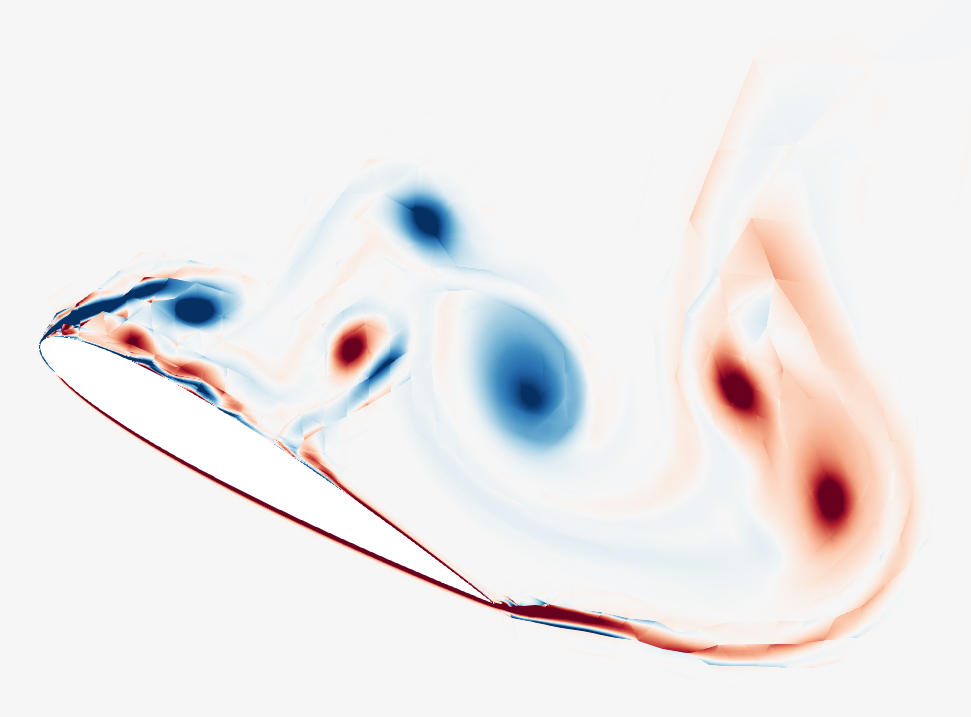
\includegraphics[width=3in]{figures/naca_vorticity}}
	\caption{Snapshot of vorticity for Reynolds 40{,}000 flow over NACA airfoil.}
\end{figure}

As a more challenging test case, we consider the Reynolds number 40{,}000 flow
over a NACA0012 airfoil. The angle of attack is $30^\circ$ and the farfield Mach
number is $0.1$. The domain is discretized using a triangular mesh with 3154
elements, and the spatial discretization is a high-order discontinuous Galerkin
method using compact stencils for the second order (viscous) terms with
polynomial degree $p=3$ \cite{Peraire2008}. No-slip boundary conditions are
enforced at the surface of the airfoil, and farfield boundary conditions at all
other domain boundaries. The main challenge associated with this problem is the
resolution of the thin boundary layer at the surface of the airfoil that results
from the no-slip condition. This boundary layer is resolved using a layer of
anisotropically stretched elements near the surface of the airfoil. These
elements result in a highly restrictive CFL stability condition, motivating the
use of implicit time integration for this problem. A time accurate time step of
$\delta t = 5 \times 10^{-2}$ is chosen for this problem. This time step is
several orders of magnitude larger than the largest stable explicit time step.
The number of nonlinear iterations and preconditioner applications required for
convergence are shown in Table \ref{tab:naca-iters}. As in the previous case,
each Krylov iteration for the SDIRK methods corresponds to a single
preconditioner application. For the IRK methods, one Krylov iteration for a
$1\times1$ system corresponds to one preconditioner application, whereas for a
$2\times2$ system, one Krylov iteration corresponds to two preconditioner
applications. As we observed in the case of the Euler vortex, the Gauss and
Radau fully implicit Runge--Kutta methods of 2, 3, and 4 converge with fewer
total preconditioner applications than the equal-order SDIRK method.

Additionally, we use this test case to compare four potential solver strategies,
corresponding to those enumerated in \Cref{sec:nonlinear:gen}. The first solver
(Solver 0) uses a simplified Newton nonlinear iteration, where the Jacobian matrix
from the first stage is used for all stages. This has the advantage that the
number of Jacobian matrix assemblies per nonlinear iteration is reduced;
however, in general, the quadratic convergence of Newton's method is not
maintained, typically resulting in an increased number of nonlinear iterations.
The remaining solvers (Solvers 1, 2, and 3) use exactly computed Jacobian
matrices at all temporal stages, and each solver corresponds to a different
approximation $\tilde{P} \approx \widehat{P}$, as described in
\Cref{sec:nonlinear:gen}. With increasing quality of the approximation, we
expect the solver to converge more rapidly, however each iteration will
generally be more expensive to compute. In \Cref{fig:naca-nonlin-solvers} we
compare the number of nonlinear iterations, number of matrix-vector products
(determined by the convergence of the Krylov solvers), number of Jacobian
assemblies, and total wall-clock runtime for these solver configurations. From
these results, we see that for this problem, the nonlinear iterations based on
better approximations lead to overall faster runtimes, despite the higher
per-iteration cost. However, we note that this performance is often
problem-dependent. In particular, for smaller time steps and less stiff
problems, the simplified Newton method can be more efficient because few Jacobian
assemblies are required, and the increase in nonlinear iterations over
Solvers 1, 2, and 3 is typically less significant.

\begin{table}
	\centering
	\caption{Nonlinear iterations and preconditioner applications for the NACA airfoil test case, with time step $\delta t = 5 \times 10^{-2}$, using Newton-like Solver 3 with a relative tolerance of $10^{-9}$.}
	\label{tab:naca-iters}
	\begin{tabular}{r|cccc|ccccc}
		\toprule
		& \multicolumn{4}{c|}{SDIRK} & \multicolumn{5}{c}{Gauss} \\
		Order  & 1 & 2 & 3 & 4 & 2 & 4 & 6 & 8 & 10\\
		\midrule
		Newton its. & 5 & 5 & 5 & 5 & 5 & 5 & 8 & 8 & 8\\
		\midrule
		Precond.\ applications & 173 & 200 & 359 & 481 & 128 & 244 & 557 & 732 & 830\\
		\bottomrule
	\end{tabular}

	\vspace{\floatsep}

	\begin{tabular}{r|cccc|ccc}
		\toprule
		& \multicolumn{4}{c|}{Radau} & \multicolumn{3}{c}{Lobatto} \\
		Order  & 3 & 5 & 7 & 9 & 2 & 6 & 8\\
		\midrule
		Newton its. & 5 & 9 & 9 & 9 & 5 & 15 & 17\\
		\midrule
		Precond.\ applications & 314 & 728 & 926 & 1061 & 454 & 1670 & 1995\\
		\bottomrule
	\end{tabular}
\end{table}

\begin{figure}
	\centering
	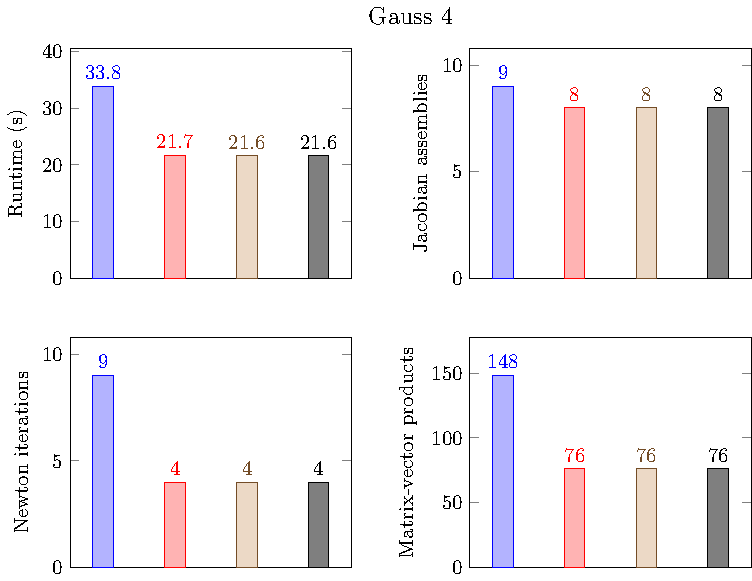
\includegraphics{figures/barchart/gauss4}

	\vspace{\floatsep}

	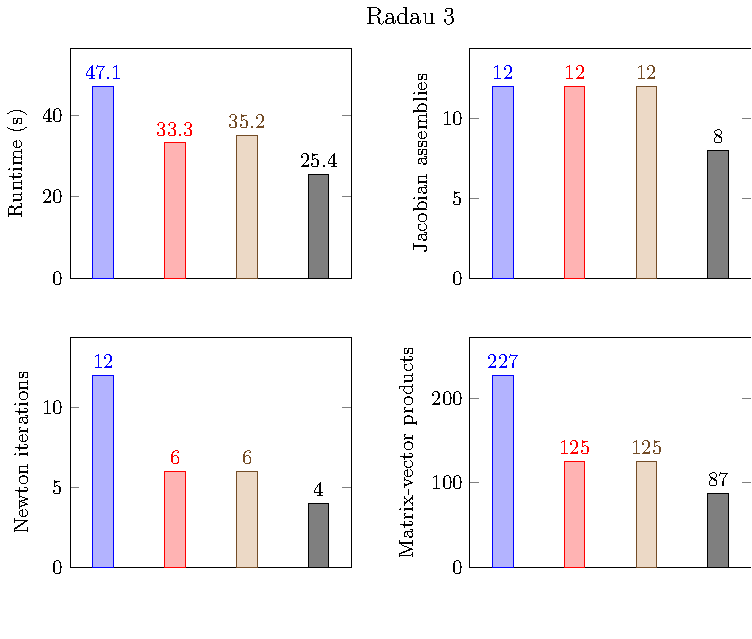
\includegraphics{figures/barchart/radau3}
	\caption{Performance for four solver configurations on the NACA test case with $\delta t = 2 \times 10^{-2}.$}
	\label{fig:naca-nonlin-solvers}
\end{figure}

% ------------------------------------------------------------------------------------- %
% ------------------------------------------------------------------------------------- %
\subsection{Incompressible Euler \& Navier--Stokes in vorticity-streamfunction form}
\label{sec:numerics:khi}

As an example of an index-1 DAE, we consider the vorticity-streamfunction formulation of the 2D incompressible Euler equations \cite{Liu2000}.
The equations are given by
\begin{align}
	\label{eq:ins-1}
	\frac{\partial\omega}{\partial t} + \nabla\cdot(\bm{u} \omega) &= 0, \\
	\label{eq:ins-2}
	\Delta \psi &= \omega,
\end{align}
where the velocity $\bm u$ is defined by $\bm u = \nabla^\perp \psi$, for $\nabla^\perp = (-\partial_y, \partial_x)$.
Here, $\omega$ is the vorticity, and $\psi$ is a scalar field known as the streamfunction, which is used to naturally enforce the divergence-free constraint on the velocity.
Note that this formulation can be easily extended to the 2D incompressible Navier--Stokes equations with the addition of a viscosity term, replacing equation \eqref{eq:ins-1} with
\begin{equation} \label{eq:ins-3}
	\frac{\partial\omega}{\partial t} + \nabla\cdot(\bm{u} \omega) = \frac{1}{\rm Re} \Delta \omega,
\end{equation}
where $\rm Re$ is the Reynolds number.
For a fixed velocity $\bm u$, equation \eqref{eq:ins-1} is a scalar advection equation for $\omega$, which we discretize using an upwind discontinuous Galerkin method.
If the streamfunction $\psi$ is in $H^1$, then the velocity $\bm u = \nabla^\perp \psi$ is automatically continuous across element interfaces, and therefore the standard upwind numerical flux is well-defined.
We therefore discretize \eqref{eq:ins-2} using a standard $H^1$-conforming finite element method.
Equal-order finite element spaces are chosen for $\omega$ and $\psi$.
In the case of the Navier--Stokes equations, we discretize the viscous term on the right-hand side of \eqref{eq:ins-3} using a standard interior penalty DG method \cite{Arnold1982}.

After performing the discretization, this system of equations can be written as
\begin{equation}
	\label{eq:ins-system}
	\left[ \begin{array}{c} M_{\rm dg} \omega_t \\ 0 \end{array} \right]
	=
	\left[ \begin{array}{cc} K(\psi) & 0 \\ M_{\rm mix} & A \end{array} \right]
	\left[ \begin{array}{c} \omega \\ \psi \end{array} \right],
\end{equation}
where $M_{\rm dg}$ represents the DG mass matrix, $M_{\rm mix}$ is the mixed
DG-$H^1$ mass matrix, $K(\psi)$ is the discretized advection (or
advection--diffusion) operator (depending the velocity $\bm u$ as a function of
$\psi$), and $A$ is the $H^1$-conforming diffusion operator. A Picard
linearization of \eqref{eq:ins-system} will result in a block-triangular system
that is of the same form as \eqref{eq:ins-system}, but using an iteratively
lagged advection operator. We use nonlinear method (1) from
\Cref{sec:nonlinear:gen}, where we permit differing operators on diagonal
blocks, but ignore non-identity off-diagonal coupling. For this problem, tests
indicated that including such coupling (methods 2 and 3) requires slightly
longer wall-clock times and do not offer significant reduction in nonlinear
iterations. Then, in the notation of \Cref{sec:dae}, we have $\mathcal{L}_u^{(i)} =
K(\psi^{(i)})$, $\mathcal{L}_w = 0$, $\mathcal{G}_u = M_{\rm mix}$, and
$\mathcal{G}_w = A$. The resulting $4\times4$ block system that arises from IRK
integration has the form
\begin{align} \label{eq:vsf-system-1}
	\begin{bmatrix}
		\eta M_{\rm dg} - \delta t K^{(i)} & \mathbf{0} & \phi M_{\rm dg} & \mathbf{0} \\
		-\delta t M_{\rm mix} & -\delta t A & \mathbf{0} & \mathbf{0} \\
		-\tfrac{\beta^2}{\phi}M_{\rm dg} & \mathbf{0} & \eta M_{\rm dg} - \delta t K^{(i+1)} & \mathbf{0} \\
		\mathbf{0} & \mathbf{0} & -\delta t M_{\rm mix} & -\delta t A
	\end{bmatrix}
	\begin{bmatrix} \bm\omega_i \\ \bm\psi_i \\ \bm\omega_{i+1} \\ \bm\psi_{i+1} \end{bmatrix}
	=
	\begin{bmatrix} \mathbf{f}_i \\ \mathbf{g}_i \\ \mathbf{f}_{i+1} \\ \mathbf{g}_{i+1} \end{bmatrix}.
\end{align}

We consider two types of preconditioners for this system.
The first is a standard block-triangular preconditioner, obtained by neglecting the term $\phi M_{\rm dg}$ term in the $(1,3)$ position, replacing the diagonal blocks by appropriate preconditioners, and using the preconditioning developed in \Cref{sec:theory}.
An alternative preconditioner is obtained by noticing that this system can be reordered to obtain the block-triangular system
\begin{align} \label{eq:vsf-system-2}
	\begin{bmatrix}
		\eta M_{\rm dg} - \delta t K^{(i)} & \phi M_{\rm dg} & \mathbf{0} & \mathbf{0} \\
		-\tfrac{\beta^2}{\phi}M_{\rm dg} & \eta M_{\rm dg} - \delta t K^{(i+1)}  & \mathbf{0}& \mathbf{0} \\
		-\delta t M_{\rm mix} & \mathbf{0} & -\delta t A & \mathbf{0} \\
		\mathbf{0} & -\delta t M_{\rm mix} & \mathbf{0} & -\delta t A
	\end{bmatrix}
	\begin{bmatrix} \bm\omega_i \\ \bm\omega_{i+1} \\ \bm\psi_i \\ \bm\psi_{i+1} \end{bmatrix}
	=
	\begin{bmatrix} \mathbf{f}_i \\ \mathbf{f}_{i+1} \\ \mathbf{g}_i \\ \mathbf{g}_{i+1} \end{bmatrix}.
\end{align}
This block-triangular system can be solved using a forward-substitution algorithm, first solving the leading $2\times2$ block for the time-dependent variables, and then solving two (independent) Poisson problems for the algebraic constraints (i.e.\ the streamfunctions).

Each of these approaches require preconditioning/inverting the diagonal blocks
in \eqref{eq:vsf-system-1}/\eqref{eq:vsf-system-2}. Poisson problems are solved
with optimal complexity using AMG preconditioners. The advection diffusion
equations defining vorticity are preconditioned using nonsymmetric AMG based on
approximate ideal restriction (AIR) \cite{Manteuffel:2019,Manteuffel:2018}. The
leading $2\times 2$ time-dependent vorticity equations are preconditioned using
the block-triangular preconditioners described in \Cref{sec:theory}, coupled
with AIR preconditioning for individual systems. For the block triangular
variation \eqref{eq:vsf-system-2}, the $2\times2$ diagonal blocks are solved to
high precision, while preconditioning diagonal blocks in \eqref{eq:vsf-system-1}
consists of \textit{one} AIR or AMG iteration. All linear and nonlinear iterations
are solved to relative residual tolerance of $10^{-9}$, typically yielding an
absolute tolerance $\sim\mathcal{O}(10^{-12})$.

\begin{figure}
	\def\dslfigwidth{1.75in}
	\centering
	\setlength{\fboxsep}{0pt}
	\begin{minipage}{\dslfigwidth}
		\centering
		\fbox{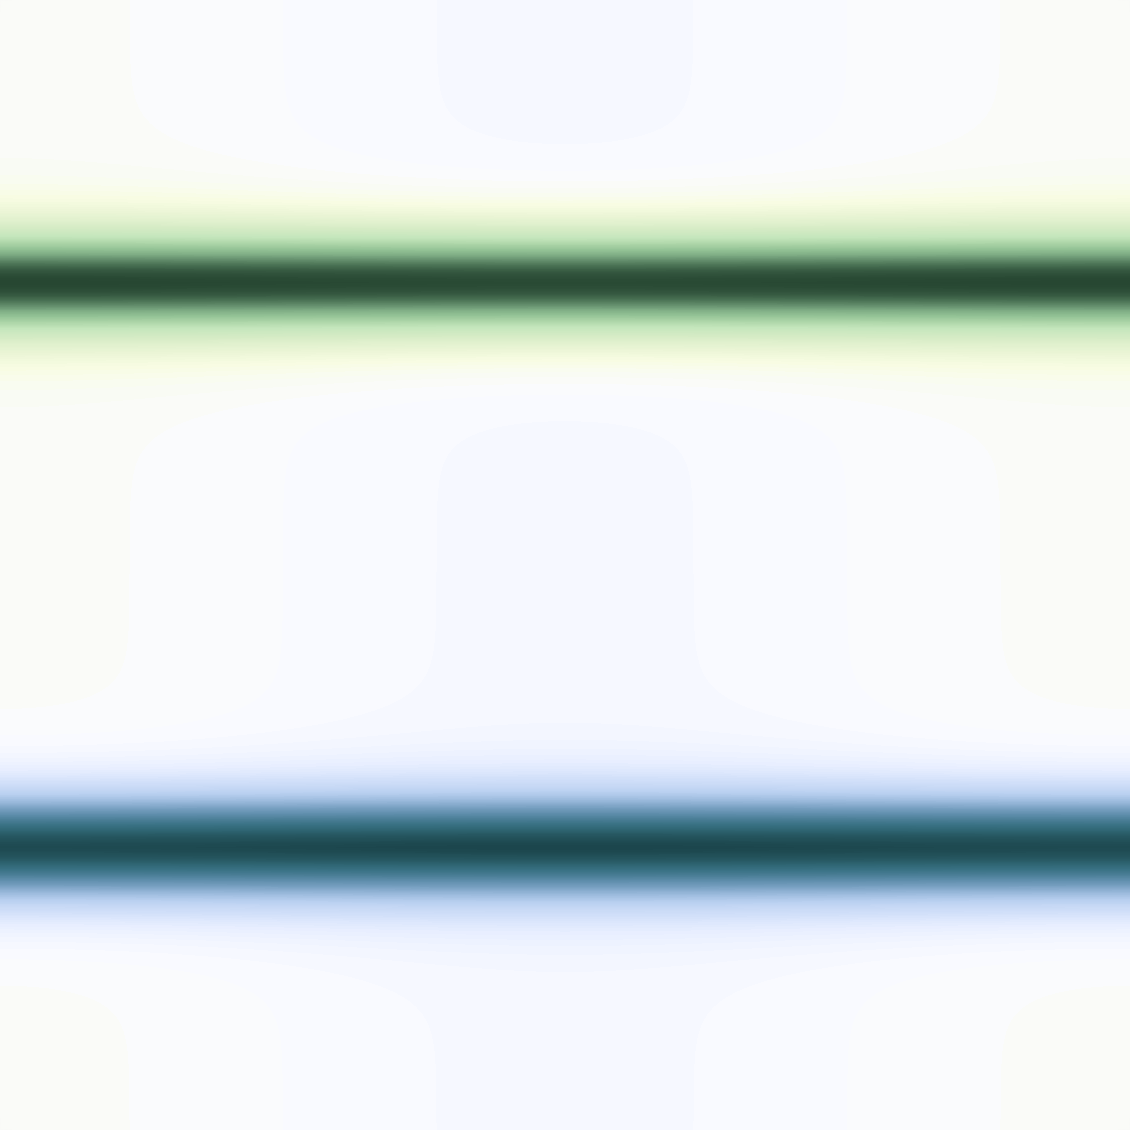
\includegraphics[width=0.99\linewidth]{figures/dsl_0000}}\\
		$t=0$
	\end{minipage}
	\hspace{0.5in}
	\begin{minipage}{\dslfigwidth}
		\centering
		\fbox{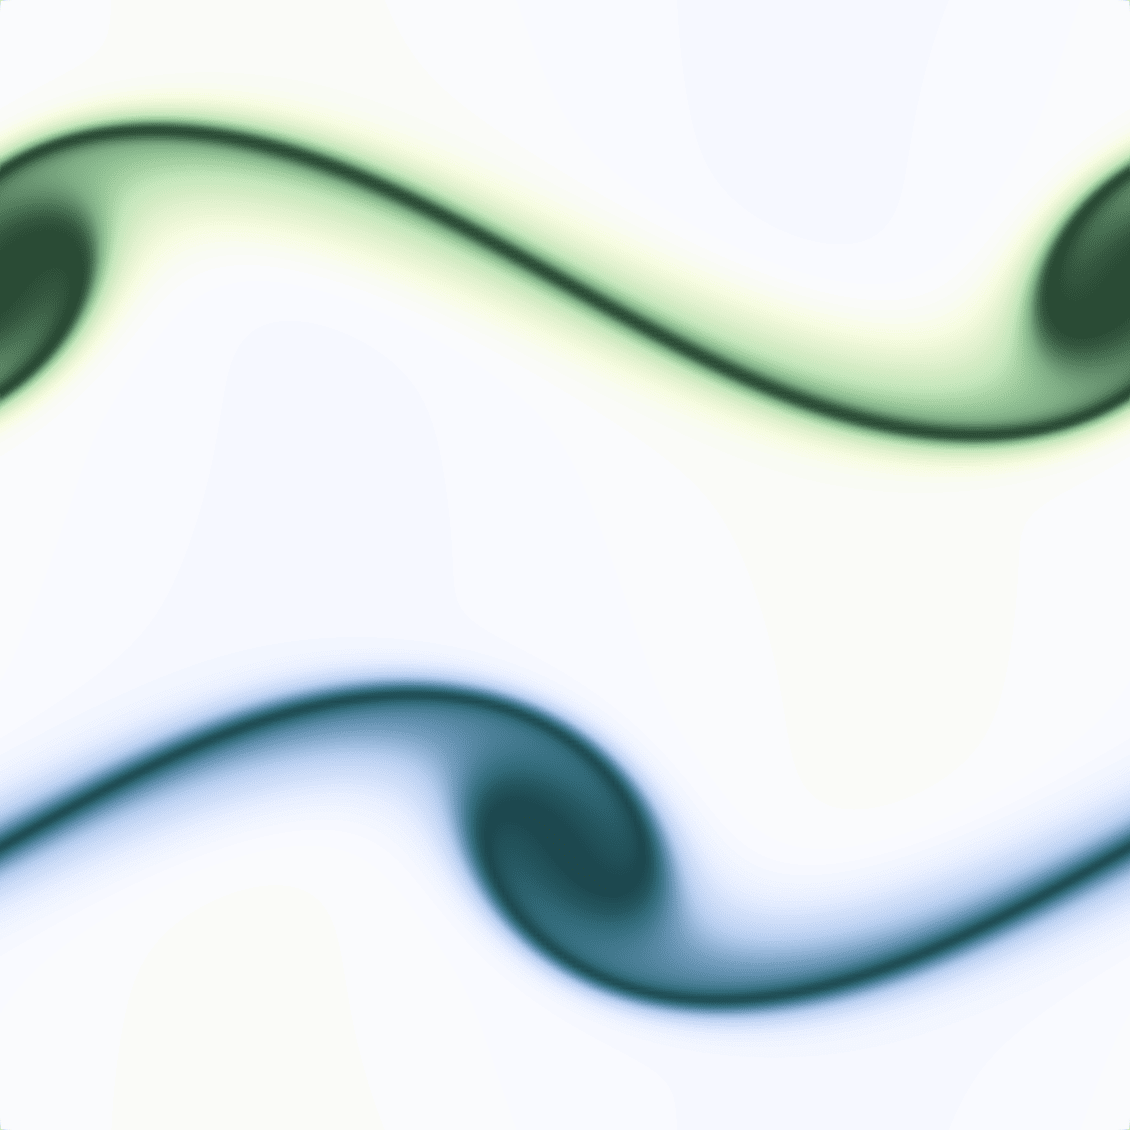
\includegraphics[width=0.99\linewidth]{figures/dsl_0250}}\\
		$t=5$
	\end{minipage}

	\vspace{\floatsep}

	\begin{minipage}{\dslfigwidth}
		\centering
		\fbox{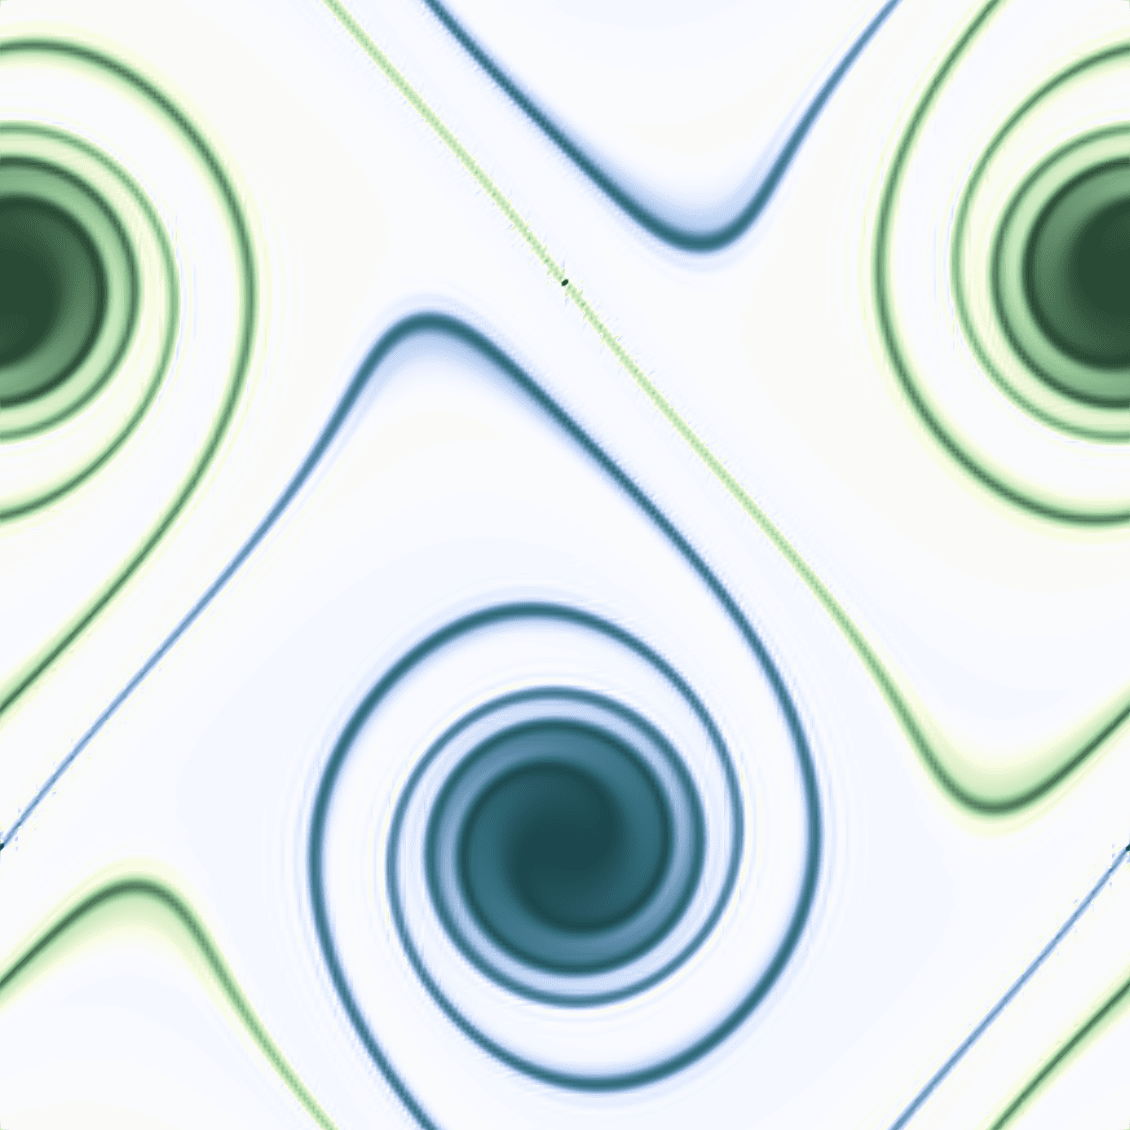
\includegraphics[width=0.99\linewidth]{figures/dsl_0500}}\\
		$t=10$
	\end{minipage}
	\hspace{0.5in}
	\begin{minipage}{\dslfigwidth}
		\centering
		\fbox{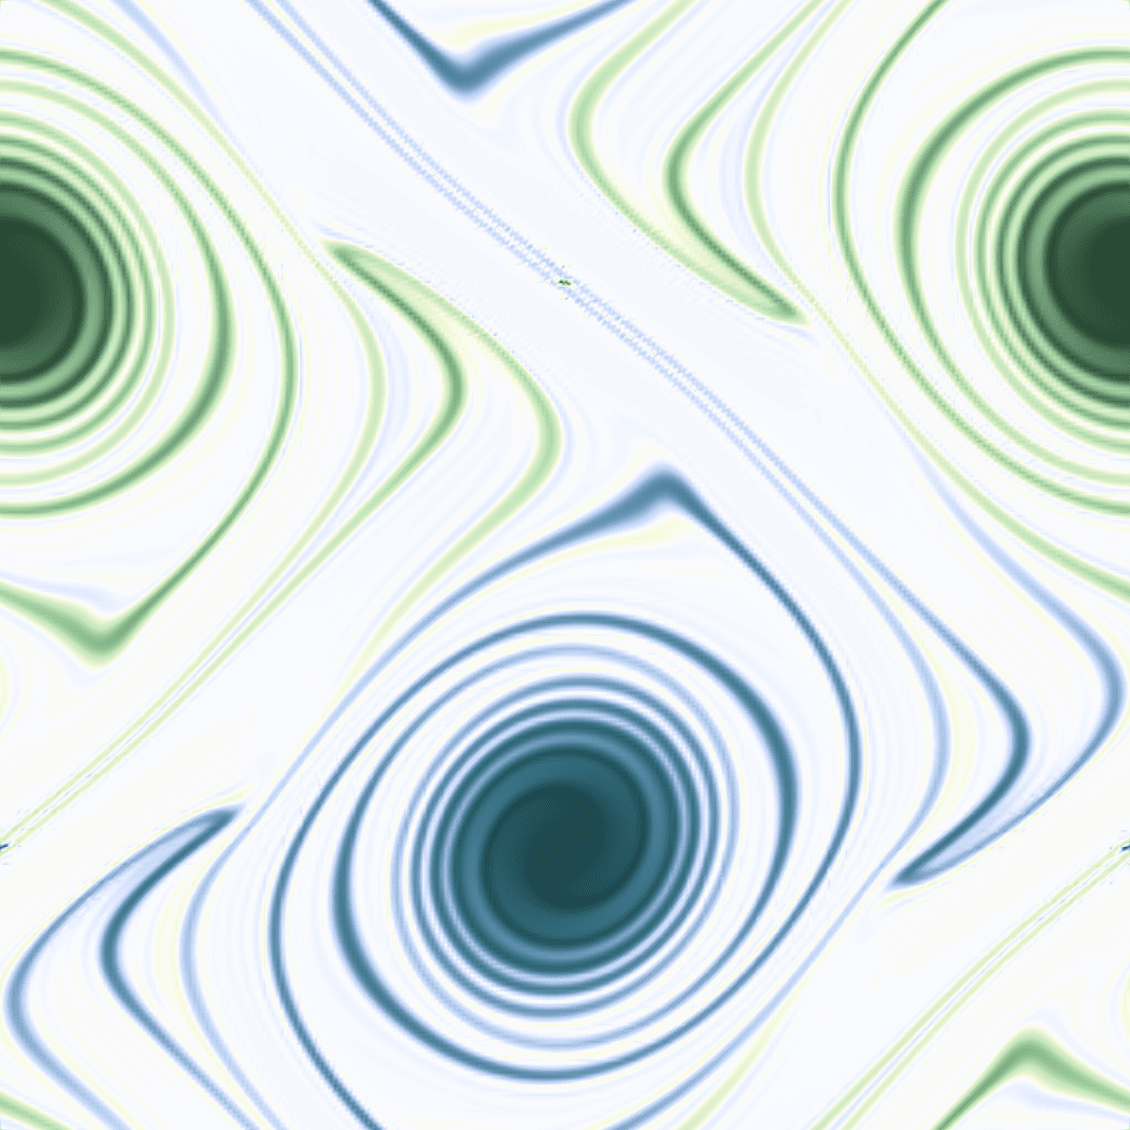
\includegraphics[width=0.99\linewidth]{figures/dsl_0750}}\\
		$t=15$
	\end{minipage}

	\caption{Time evolution of vorticity for the double shear layer problem.}
	\label{fig:dsl}
\end{figure}

To study the effectiveness of these preconditioners, we consider the double shear layer problem \cite{Bell1989}.
The domain is taken to be the square $[0,2\pi] \times [0,2\pi]$, and periodic boundary conditions are enforced at the domain boundaries.
The initial condition is given by
\[
	\omega(x,y,0) = \begin{cases}
		\delta \cos(x) - \frac{1}{\rho}\operatorname{sech}^2((y-\pi/2)/\rho) \qquad & y \leq \pi, \\
		\delta \cos(x) + \frac{1}{\rho}\operatorname{sech}^2((3\pi/2 - y) \qquad & y > \pi.
	\end{cases}
\]
This test case is well-suited for high-order methods because the solution quickly develops small-scale features, as shown in \Cref{fig:dsl}.
We use finite element spaces with polynomial degree $p=3$, mesh spacing $h = 0.0025$, and choose a time step of $\delta t = 10^{-2}$ for all RK schemes to consider scalability in integration order for fixed $\delta t$.
\Cref{tab:dsl-iters} shows the total number of preconditioner applications required per time step with Reynolds number Re  $=10$. Rows indicated ``Prec.\ applications'' correspond to \eqref{eq:vsf-system-1}, and each preconditioner application is defined as preconditioning a $2\times 2$ block over $[\boldsymbol{\omega}_i,\boldsymbol{\psi}_i]$ with {one} AIR iteration and one AMG iteration (one for each diagonal block). The block triangular variation \eqref{eq:vsf-system-2} does a block forward solve on \eqref{eq:vsf-system-2}, and \Cref{tab:dsl-iters} presents the total number of AIR and AMG iterations required for the forward solve, summed over all nonlinear iterations.
Note, because the time-dependent and algebraic blocks are solved separately in this case, the number of AIR iterations (to solve for the vorticity) and AMG iterations (to solve for the streamfunction) are not equal. These results were run on 288 cores on the Quartz machine at Lawrence Livermore National Laboratory.

\begin{table}[h!]
	\centering
	\caption{Preconditioner applications for the double shear layer test case, with third-order
	finite elements, mesh spacing $h=0.0025$, time step $\delta t = 10^{-2}$, and Re $=10$. One
	``Prec. application'' corresponds to one AIR iteration and one AMG iteration.}
	\label{tab:dsl-iters}
	\begin{tabular}{rl|cccc|ccccc}
		\toprule
		&& \multicolumn{4}{c|}{SDIRK} & \multicolumn{5}{c}{Gauss} \\
		& \multicolumn{1}{r|}{Order}  & 1 & 2 & 3 & 4 & 2 & 4 & 6 & 8 & 10\\
		\midrule
		\eqref{eq:vsf-system-1} & Prec.\ applications & 127 & 141 & 322 & 365 & 78 & 161 & 218 & 287 & 333 \\
		\midrule
		\multirow{2}{*}{\eqref{eq:vsf-system-2}} & AIR iterations & 127 & 141 & 322 & 365 & 78 & 365 & 538 & 731 & 1064\\
		& AMG iterations & 127 & 141 & 322 & 365 & 78 & 368 & 562 & 766 & 1204 \\
		\bottomrule
	\end{tabular}

	\vspace{\floatsep}

	\begin{tabular}{rl|cccc|cccc}
		\toprule
		&& \multicolumn{4}{c|}{Radau} & \multicolumn{4}{c}{Lobatto} \\
		& \multicolumn{1}{r|}{Order} & 3 & 5 & 7 & 9 & 2 & 4 & 6 & 8\\
		\midrule
		\eqref{eq:vsf-system-1} & Prec.\ applications & 237 & 232 & 299 & 490 & 217 & 234 & 311 & 375 \\
		\midrule
		\multirow{2}{*}{\eqref{eq:vsf-system-2}} & AIR iterations & 451 & 603 & 841 & 989 & 421 & 697 & 2013 & 1405 \\
		& AMG iterations & 432 & 566 & 819 & 980 & 350 & 670 & 1580 & 1227\\
		\bottomrule
	\end{tabular}
\end{table}

Note from \Cref{tab:dsl-iters} that the second and fourth order Gauss methods
are significantly more efficient than the corresponding equal-order SDIRK
methods in terms of total number of preconditioner applications, while the
\textit{10th-order} Gauss method requires approximately as many (in fact,
slightly less) preconditioner applications per time step as the fourth-order
SDIRK method. In all cases, the triangular nonlinear preconditioning
\eqref{eq:vsf-system-2} requires many more iterations than the more general
approach following the development in this paper \eqref{eq:vsf-system-1}. This
is largely because the linear preconditioning ends up being more efficient
when applied to the full system \eqref{eq:vsf-system-1}, rather than the
reordered system in \eqref{eq:vsf-system-2}. Moreover, linear iteration
counts are almost equal for nonlinear methods 1, 2, and 3 (results are not
shown for sake of space) from \Cref{sec:nonlinear:gen}, indicating that=
linear conditioning theory developed in \Cref{sec:theory:gen} for systems
that arise from nonlinear method 1 yields robust preconditioners for
methods 2 and 3 as well.

\Cref{tab:dsl-iters2} demonstrates that the proposed methods are also robust
across Reynolds number, showing similar results as in \Cref{tab:dsl-iters}, for
the preconditioning in \eqref{eq:vsf-system-1} with Reynolds number 25,000.  As
before, Gauss methods require roughly half the preconditioner applications as
required by equal order SDIRK methods, while 4th-order SDIRK requires almost as many
preconditioner applications as 10th-order Gauss, and more than 8th-order Gauss and
7th-order Radau IIA.

\begin{table}[h!]
	\centering
	\caption{Preconditioner applications for the double shear layer test case, with third-order
	finite elements, mesh spacing $h=0.0025$, time step $\delta t = 10^{-2}$, and Re $=25,000$.
	One ``Prec. application'' corresponds to one AIR iteration and one AMG iteration.}
	\label{tab:dsl-iters2}
	\begin{tabular}{rl|cccc|ccccc}
		\toprule
		&& \multicolumn{4}{c|}{SDIRK} & \multicolumn{5}{c}{Gauss} \\
		& \multicolumn{1}{r|}{Order}  & 1 & 2 & 3 & 4 & 2 & 4 & 6 & 8 & 10\\
		\midrule
		\eqref{eq:vsf-system-1} & Prec.\ applications & 41 & 72 & 113 & 177 & 37 & 75 & 118 & 163 & 194 \\
		\bottomrule
	\end{tabular}

	\vspace{\floatsep}

	\begin{tabular}{rl|cccc|cccc}
		\toprule
		&& \multicolumn{4}{c|}{Radau} & \multicolumn{4}{c}{Lobatto} \\
		& \multicolumn{1}{r|}{Order} & 3 & 5 & 7 & 9 & 2 & 4 & 6 & 8\\
		\midrule
		\eqref{eq:vsf-system-1} & Prec.\ applications & 81 & 123 & 165 & 206 & 91 & 130 & 173 & 220 \\
		\bottomrule
	\end{tabular}
\end{table}

To assess the accuracy of IRK methods applied to this problem, we consider the
integration of the double shear layer problem over a longer time interval of
$[0,10]$. We choose a Reynolds number of 100, and compute a reference solution
by applying explicit 6th-order SDIRK integration with a small time step of
$\delta t = 10^{-4}$. We then apply IRK methods with large time steps of
$\delta t \in\{0.4,0.2,0.1\}$ and observe the orders of convergence in
\Cref{tab:tgv-errors}. As a consequence of the nonlinear solver tolerance
of $10^{-11}$, the observed order of convergence is reduced for the highest
order methods and the refinement $\delta t =0.2 \mapsto \delta t=0.1$.
Nevertheless, we observe that each of the methods indeed yield high-order
accuracy using very large time steps, in most cases just under their formal
order of accuracy. Moreover, the leading error constants also appear to be
small, given we can obtain accuracy on the order of $10^{-9}-10^{-10}$ with
a step size of $\delta t = 0.2$. Similar results have been observed on the
Taylor Green vortex problem; here we use the double shear layer problem to
demonstrate high-order accuracy on a problem with more interesting long-term
dynamics.

\begin{table}[h!]
	\centering
	\caption{Error and convergence rates for double shear layer problem with Re$=10$.}
	\label{tab:tgv-errors}
	\begin{tabular}{r|cccccc}
		\toprule
		& \multicolumn{2}{c}{Gauss 4} & \multicolumn{2}{c}{Gauss 6} & \multicolumn{2}{c}{Gauss 8}\\
		$\delta t$ & Error & Rate & Error & Rate & Error & Rate\\
		\midrule
		0.4 & $1.98\times 10^{-3}$ & --- & $1.59\times 10^{-4}$ & --- & $4.13\times 10^{-5}$ & --- \\
		0.2 & $1.30\times 10^{-4}$ & 3.93 & $9.08\times 10^{-7}$ & 7.45 & $1.04\times 10^{-8}$ & 11.95 \\
		0.1 & $8.15\times 10^{-6}$ & 3.99 & $9.29\times 10^{-9}$ & 6.61 & $1.05\times 10^{-10}$ & 6.63 \\
		\midrule
		& \multicolumn{2}{c}{Radau 5} & \multicolumn{2}{c}{Radau 7} & \multicolumn{2}{c}{Radau 9}\\
		\midrule
		0.4 & $2.37\times 10^{-4}$ & --- & $3.96\times 10^{-6}$ & --- & $6.21\times 10^{-8}$ & --- \\
		0.2 & $8.35\times 10^{-6}$ & 4.83 & $3.54\times 10^{-8}$ & 6.81 & $1.42\times 10^{-10}$ & 8.77  \\
		0.1 & $2.71\times 10^{-7}$ & 4.94 & $2.93\times 10^{-10}$ & 6.91 & $3.64\times 10^{-11}$ & 1.96 \\
		\midrule
		& \multicolumn{2}{c}{Lobatto 4} & \multicolumn{2}{c}{Lobatto 6} & \multicolumn{2}{c}{Lobatto 8}\\
		\midrule
		0.4 & $2.42\times 10^{-3}$ & --- & $3.93\times 10^{-5}$ & --- & $6.15\times 10^{-7}$ & --- \\
		0.2 & $1.78\times 10^{-4}$ & 3.76 & $7.23\times 10^{-7}$ & 5.77 & $2.86\times 10^{-9}$ & 7.75 \\
		0.1 & $1.18\times 10^{-5}$ & 3.92 & $1.19\times 10^{-8}$ & 5.91 & $3.62\times 10^{-11}$ & 6.30 \\
		\bottomrule
	\end{tabular}
\end{table}

%
\begin{comment}
To assess the accuracy of IRK methods applied to this problem, we consider the two-dimensional incompressible Taylor--Green vortex problem.
As in the previous case, the domain is taken to be the periodic square $[0,2\pi]^2$.
The initial conditions are given by
\[
	\omega(x,y,0) = -2\sin(x)\sin(y).
\]
These initial conditions are a steady solution for the incompressible Euler equations.
For this problem, we consider the Navier--Stokes equations, for which the exact solution is given by
\[
	\omega(x,y,t) = -2\sin(x)\sin(y) \exp(-2t/\rm Re).
\]
An advantage of implicit time integration for this problem is that the scheme remains stable even for small Reynolds numbers.
As such, we choose $\rm Re = 10$ for this problem, and integrate until $t = 0.1$.
We compare the numerical solutions with a reference solution computed using a small time step of $\delta t = 10^{-5}$.
The results are presented in \Cref{tab:tgv-errors}.
As a consequence of the nonlinear solver tolerance, the observed order of convergence is slightly reduced for the sixth and seventh order Lobatto and Radau methods.

\begin{table}
	\centering
	\caption{Error and convergence rates for Taylor--Green vortex problem}
	\label{tab:tgv-errors}
	\begin{tabular}{r|cccccc}
		\toprule
		& \multicolumn{2}{c}{Gauss 2} & \multicolumn{2}{c}{Gauss 4} & \multicolumn{2}{c}{Gauss 6}\\
		$\delta t$ & Error & Rate & Error & Rate & Error & Rate\\
		\midrule
		$3.20\times 10^{-2}$ & $1.96 \times 10^{-5}$ & --- & $2.30 \times 10^{-6}$ & --- & $3.45 \times 10^{-8}$ & --- \\
		$1.60\times 10^{-2}$ & $7.10 \times 10^{-6}$ & 1.47 & $1.10 \times 10^{-7}$ & 4.38 & $8.70 \times 10^{-11}$ & 8.63 \\
		\midrule
		& \multicolumn{2}{c}{Radau 3} & \multicolumn{2}{c}{Radau 5} & \multicolumn{2}{c}{Radau 7}\\
		\midrule
		$3.20\times 10^{-2}$ & $2.18 \times 10^{-8}$ & --- & $9.52 \times 10^{-10}$ & --- & $7.78 \times 10^{-11}$ & --- \\
		$1.60\times 10^{-2}$ & $3.17 \times 10^{-9}$ & 2.78 & $2.92 \times 10^{-11}$ & 5.03 & $1.61 \times 10^{-12}$ & 5.60 \\
		\midrule
		& \multicolumn{2}{c}{Lobatto 2} & \multicolumn{2}{c}{Lobatto 4} & \multicolumn{2}{c}{Lobatto 6}\\
		\midrule
		$3.20\times 10^{-2}$ & $8.11 \times 10^{-7}$ & --- & $4.68 \times 10^{-9}$ & --- & $1.26 \times 10^{-10}$ & --- \\
		$1.60\times 10^{-2}$ & $2.05 \times 10^{-7}$ & 1.99 & $3.82 \times 10^{-10}$ & 3.62 & $2.36 \times 10^{-12}$ & 5.73 \\
		\bottomrule
	\end{tabular}
\end{table}
\end{comment}
%


% \subsection{(Incompressible) Kelvin-Helmholtz instability}\label{sec:numerics:khi}
% Define $\mathbf{v}$ as a curl, such that $\nabla \cdot\mathbf{v}w =
% \mathbf{v}\cdot\nabla w$, and
% consider the equations
% %
% \begin{align}\label{eq:2dfluid}
% \begin{split}
% \partial_t w + \mathbf{v}\cdot\nabla w - \nabla_\perp \cdot\mu\nabla_\perp w & = 0, \\
% -\nabla_\perp^2\phi + w & = 0, \\
% \mathbf{v} + \nabla \times \phi\hat{\mathbf{z}} & = \mathbf{0}.
% \end{split}
% \end{align}
% %
% Here $\mu$ is a fixed (spatially dependent) diffusion constant or tensor, and $\nabla_\perp$
% indicates the gradient in the $xy$-plane. $\mathbf{v}$ is the drift velocity, and is a nonlinear
% coupling in the time propagation of \eqref{eq:2dfluid}. Equation \eqref{eq:2dfluid} can
% be represented as a $3\times 3$ block set of equations with nonlinearity in the leading block,
% %
% \begin{align}\label{eq:block_khi}
% \begin{bmatrix} \partial_t w \\ 0 \\ \mathbf{0}\end{bmatrix} =
% \begin{bmatrix} {N}(\mathbf{v}) + \nabla_\perp \cdot\mu\nabla_\perp &
% 		\mathbf{0} & \mathbf{0} \\
% 	-M_w &  \nabla_\perp^2 & \mathbf{0} \\ \mathbf{0} & \nabla\times \mathbf{z} & M_{\mathbf{v}}
% \end{bmatrix}
% 	\begin{bmatrix} w \\ \phi \\ \mathbf{v}\end{bmatrix} ,
% \end{align}
% %
% where $N(\mathbf{v}) := -\mathbf{v}\cdot\nabla$.

% A Picard linearization of the nonlinear operator in \eqref{eq:block_khi} takes
% the simple block lower triangular form,
% %
% \begin{align}\label{eq:dae_pic}
% L[w_k,\phi_k,\mathbf{v}_k] :=
% 	\begin{bmatrix} \mathbf{v}_k\cdot\nabla + \nabla_\perp \cdot\mu\nabla_\perp &
% 		\mathbf{0} & \mathbf{0} \\
% 	-M_w &  \nabla_\perp^2 & \mathbf{0} \\ \mathbf{0} & \nabla\times \mathbf{z} & M_{\mathbf{v}}
% \end{bmatrix}
% \end{align}
% %
% Now, let us swap the rows and columns of $\phi$ and $\mathbf{v}$. Then, a
% Newton linearization can be expressed in strong form as the Jacobian as a
% function of previous nonlinear iterates,
% %
% \begin{align*}
% J[w_k,\mathbf{v}_k, \phi_k] :=
% 	\begin{bmatrix} \mathbf{v}_k\cdot\nabla + \nabla_\perp \cdot\mu\nabla_\perp &
% 		(\nabla w_k)\cdot  & \mathbf{0} \\
% 	\mathbf{0} & M_{\mathbf{v}} & \nabla\times \mathbf{z} \\
% 	-M_w & \mathbf{0} & \nabla_\perp^2 \\
% \end{bmatrix}.
% \end{align*}
% %
% A reasonable Newton-like method would be to ignore the weak mass-matrix
% coupling between $w$ and $\phi$ and consider the block upper triangular
% nonlinear preconditioning,
% %
% \begin{align}\label{eq:dae_jac}
% \widehat{J}[w_k,\mathbf{v}_k, \phi_k] :=
% 	\begin{bmatrix} \mathbf{v}_k\cdot\nabla + \nabla_\perp \cdot\mu\nabla_\perp &
% 		(\nabla w_k)\cdot  & \mathbf{0} \\
% 	\mathbf{0} & M_{\mathbf{v}} & \nabla\times \mathbf{z} \\
% 	\mathbf{0} & \mathbf{0} & \nabla_\perp^2 \\
% \end{bmatrix}.
% \end{align}
% %

% Note that in both \eqref{eq:dae_pic} and \eqref{eq:dae_jac}, one of the
% off-diagonal blocks coupling time-dependent variables with algebraic
% constraints is zero (in the notation of \Cref{sec:dae}, either
% $\mathcal{L}_{w}=\mathbf{0}$ \eqref{eq:dae_pic} or $\mathcal{G}_{u} = \mathbf{0}$
% \eqref{eq:dae_jac}). Without loss of generality, consider the Picard
% linearization \eqref{eq:dae_pic} -- the $4\times 4$ block linear system
% \eqref{eq:dae_block} that arises in IRK integration can be reordered
% to take the block lower triangular form
% %
% \begin{align}\label{eq:dae_block_pic}
% \begin{bmatrix} \eta M - \delta t\mathcal{L}_{u}^{(1)} & \phi M & \mathbf{0} & \mathbf{0} \\
% 	-\tfrac{\beta^2}{\phi}M & \eta M - \delta t\mathcal{L}_{u}^{(2)} & \mathbf{0} & \mathbf{0} \\
% 	-\delta t\mathcal{G}_{u}^{(1)} & \mathbf{0} & -\delta t\mathcal{G}_w^{(1)} & \mathbf{0} \\
% 	\mathbf{0} & -\delta t\mathcal{G}_{u}^{(2)}  & \mathbf{0} &
% 		-\delta t\mathcal{G}_w^{(2)} \end{bmatrix}
% 	\begin{bmatrix} \mathbf{k}_1 \\ \mathbf{k}_2 \\
% 		\boldsymbol{\ell}_1 \\ \boldsymbol{\ell}_2 \end{bmatrix}
% 	= 	\begin{bmatrix} \mathbf{f}_1 \\ \mathbf{f}_2 \\
% 		 \mathbf{g}_1 \\ \mathbf{g}_2 \end{bmatrix}.
% \end{align}
% %
% where $\mathcal{L}_{u}\sim \mathbf{v}_k\cdot\nabla + \nabla_\perp \cdot\mu\nabla_\perp$,
% $\mathcal{G}_{u} \sim [-M_w;\mathbf{0}]$, and $\mathcal{G}_w\sim
% \begin{bmatrix} \nabla_\perp^2 & \mathbf{0} \\ \nabla\times \mathbf{z} & M_{\mathbf{v}}
% \end{bmatrix}$. Here, the theory and $2\times 2$ preconditioners developed in
% \Cref{sec:theory} can be applied to invert the leading $2\times 2$ block in
% \eqref{eq:dae_block_pic}, and the algebraic constraints can then be
% applied by inverting $\mathcal{G}_w^{(1)}$ and $\mathcal{G}_w^{(2)}$,
% exactly as would be done in DIRK integration. Analogous results hold
% for the Newton-like iteration \eqref{eq:dae_jac}, but the resulting system
% ends up being upper triangular. There, the algebraic constraints are
% enforced first and the leading $2\times 2$ block in \eqref{eq:dae_block_pic}
% then inverted to update the time-dependent variable.



% ------------------------------------------------------------------------------------- %
% ------------------------------------------------------------------------------------- %
% ------------------------------------------------------------------------------------- %
\section{Conclusions}\label{sec:conc}

This paper introduces a theoretical and algorithmic framework for the fast, parallel
solution of fully implicit Runge-Kutta methods in numerical PDEs. Multiple approximate
linearizations are developed, and linear algebra theory is derived to guarantee
fast and effective block preconditioning techniques for the linearized systems,
guaranteeing $\mathcal{O}(1)$ conditioning and only requiring standard preconditioners
as would be used for backward Euler time integration. The new methods are shown to achieve fast,
high-order accuracy on multiple different compressible and incompressible Navier
Stokes and Euler problems. Using low-order Gauss integration schemes
with the new method consistently requires about half the preconditioner applications as
required by standard SDIRK schemes to achieve the same accuracy, demonstrating that
the new method can not only offer very high-order accuracy (along with other benefits
obtained by using fully implicit Runge-Kutta), but also improve upon state-of-the-art
low-order integration. Moreover, for the incompressible Navier Stokes double shear
layer problem in vorticity-streamfunction form, one can apply 7th to 10th order Gauss
or Radau IIA integration for a comparable number of preconditioner applications as
standard 4th-order SDIRK.

% % ------------------------------------------------------------------------------------- %
% % ------------------------------------------------------------------------------------- %
% % ------------------------------------------------------------------------------------- %
% \section*{Appendix}

% % ------------------------------------------------------------------------------------- %
% % ------------------------------------------------------------------------------------- %
% \subsection{Real Schur decomposition applied to general operators}

% Here we write out $(Q_0^T\otimes I)\boldsymbol{\mathcal{L}}(Q_0\otimes I)$
% in bracket notation, where, e.g., $\{a_1,a_2,a_3\}\mapsto a_1\mathcal{L}_1 + a_2\mathcal{L}_2 +
% a_3\mathcal{L}_3$. Note in the matrices below, the constants in diagonal brackets always
% sum to one and off-diagonal sum to zero, wherein if $\mathcal{L}_i = \mathcal{L}_j$ for
% all $i,j$, each of the following operators is the identity.

% % ------------------------------------------------------------------------------------- %
% \subsubsection*{Gauss}

% %
% \textbf{2-stage:}
% \begin{align*}
% \begin{bmatrix}
% \{1,0\} & \{0,0\} \\
%  \{0,0\} & \{0,1\} \\
% \end{bmatrix}
% \end{align*}
% %
% \textbf{3,-stage:}
% \begin{align*}
% \begin{bmatrix}
% \{0.002,0.565,0.432\} & \{-0.038,-0.245,0.284\} & \{0.024,-0.430,0.405\}\\
% \{-0.038,-0.245,0.284\} & \{0.705,0.107,0.187\} & \{-0.453,0.187,0.266\}\\
% \{0.024,-0.430,0.405\} & \{-0.453,0.187,0.266\} & \{0.291,0.327,0.380\}\\
% \end{bmatrix}
% \end{align*}
% %
% \textbf{4,-stage:}
% \begin{align*}
% \begin{bmatrix}
% \{0.002,0.014,0.012,0.970\} & \{0.001,-0.011,-0.110,0.120\} & \{-0.016,-0.113,0.010,0.119\} & \{-0.045,0.041,-0.005,0.009\}\\
% \{0.001,-0.011,-0.110,0.120\} & \{0.000,0.008,0.975,0.014\} & \{-0.007,0.085,-0.093,0.014\} & \{-0.021,-0.031,0.051,0.001\}\\
% \{-0.016,-0.113,0.010,0.119\} & \{-0.007,0.085,-0.093,0.014\} & \{0.113,0.863,0.008,0.014\} & \{0.316,-0.312,-0.004,0.001\}\\
% \{-0.045,0.041,-0.005,0.009\} & \{-0.021,-0.031,0.051,0.001\} & \{0.316,-0.312,-0.004,0.001\} & \{0.883,0.113,0.002,0.000\}\\
% \end{bmatrix}
% \end{align*}


% %,-,-,-,-,-,-,-,-,-,-,-,-,-,-,-,-,-,-,-,-,-,-,-,-,-,-,-,-,-,-,-,-,-,-,-,-,-,-,-,-,-,-,-,-,-,-,-,-,-,-,-,-,-,-,-,-,-,-,-,-,-,-,-,-,-,-,-,-,-,-,-,-,-,-,-,-,-,-,-,-,-,-,-,-,-%
% \subsubsection*{Radau IIA}

% %
% \textbf{2,-stage:}
% \begin{align*}
% \begin{bmatrix}
% \{0.985,0.014\} & \{0.121,-0.121\}\\
% \{0.121,-0.121\} & \{0.014,0.985\}\\
% \end{bmatrix}
% \end{align*}
% %
% \textbf{3,-stage:}
% \begin{align*}
% \begin{bmatrix}
% \{0.019,0.052,0.928\} & \{0.006,0.222,-0.229\} & \{0.137,-0.017,-0.119\}\\
% \{0.006,0.222,-0.229\} & \{0.002,0.941,0.056\} & \{0.045,-0.075,0.029\}\\
% \{0.137,-0.017,-0.119\} & \{0.045,-0.075,0.029\} & \{0.978,0.006,0.015\}\\
% \end{bmatrix}
% \end{align*}
% %
% \textbf{4,-stage:}
% \begin{align*}
% \begin{bmatrix}
% \{0.002,0.031,0.103,0.862\} & \{0.006,0.022,-0.301,0.272\} & \{0.052,-0.049,0.025,-0.028\} & \{-0.014,-0.166,-0.029,0.209\}\\
% \{0.006,0.022,-0.301,0.272\} & \{0.015,0.016,0.882,0.085\} & \{0.120,-0.035,-0.075,-0.009\} & \{-0.032,-0.118,0.084,0.066\}\\
% \{0.052,-0.049,0.025,-0.028\} & \{0.120,-0.035,-0.075,-0.009\} & \{0.915,0.077,0.006,0.000\} & \{-0.245,0.260,-0.007,-0.006\}\\
% \{-0.014,-0.166,-0.029,0.209\} & \{-0.032,-0.118,0.084,0.066\} & \{-0.245,0.260,-0.007,-0.006\} & \{0.066,0.874,0.008,0.050\}\\
% \end{bmatrix}
% \end{align*}

% ------------------------------------------------------------------------------- %
\bibliographystyle{siamplain}
\bibliography{refs2.bib}


\end{document}


ADJUGATE FORMS, b^T * A0^{-1} * Adj(Ms)
Let M = A0^{-1}, with entries {m_ij}, b = b[b1,...,bs], and xx = spatial operator L

Stiffly accurate RK (b0^TA0^{-1} = [0,...,0,1])
-----------------------------------------------
s = 2
  -m21,
  m11 - xx

s = 3
  -m22 m31 + m21 m32 + m31 xx,
  m12 m31 - m11 m32 + m32 xx,
  -m12 m21 + m11 m22 - m11 xx - m22 xx + xx^2

s = 4
  m23 m32 m41 - m22 m33 m41 - m23 m31 m42 + m21 m33 m42 + m22 m31 m43 -
	 m21 m32 m43 + m22 m41 xx + m33 m41 xx - m21 m42 xx - m31 m43 xx -
	 m41 xx^2,
  -m13 m32 m41 + m12 m33 m41 + m13 m31 m42 - m11 m33 m42 -
	 m12 m31 m43 + m11 m32 m43 - m12 m41 xx + m11 m42 xx + m33 m42 xx -
	 m32 m43 xx - m42 xx^2,
  m13 m22 m41 - m12 m23 m41 - m13 m21 m42 + m11 m23 m42 + m12 m21 m43 -
	 m11 m22 m43 - m13 m41 xx - m23 m42 xx + m11 m43 xx + m22 m43 xx -
	 m43 xx^2,
  -m13 m22 m31 + m12 m23 m31 + m13 m21 m32 - m11 m23 m32 -
	 m12 m21 m33 + m11 m22 m33 + m12 m21 xx - m11 m22 xx + m13 m31 xx +
	 m23 m32 xx - m11 m33 xx - m22 m33 xx + m11 xx^2 + m22 xx^2 +
	 m33 xx^2 - xx^3

s = 5
  m24 m33 m42 m51 - m23 m34 m42 m51 - m24 m32 m43 m51 +
	  m22 m34 m43 m51 + m23 m32 m44 m51 - m22 m33 m44 m51 -
	  m24 m33 m41 m52 + m23 m34 m41 m52 + m24 m31 m43 m52 -
	  m21 m34 m43 m52 - m23 m31 m44 m52 + m21 m33 m44 m52 +
	  m24 m32 m41 m53 - m22 m34 m41 m53 - m24 m31 m42 m53 +
	  m21 m34 m42 m53 + m22 m31 m44 m53 - m21 m32 m44 m53 -
	  m23 m32 m41 m54 + m22 m33 m41 m54 + m23 m31 m42 m54 -
	  m21 m33 m42 m54 - m22 m31 m43 m54 + m21 m32 m43 m54 -
	  m23 m32 m51 xx + m22 m33 m51 xx - m24 m42 m51 xx - m34 m43 m51 xx +
	  m22 m44 m51 xx + m33 m44 m51 xx + m23 m31 m52 xx - m21 m33 m52 xx +
	  m24 m41 m52 xx - m21 m44 m52 xx - m22 m31 m53 xx + m21 m32 m53 xx +
	  m34 m41 m53 xx - m31 m44 m53 xx - m22 m41 m54 xx - m33 m41 m54 xx +
	  m21 m42 m54 xx + m31 m43 m54 xx - m22 m51 xx^2 - m33 m51 xx^2 -
	  m44 m51 xx^2 + m21 m52 xx^2 + m31 m53 xx^2 + m41 m54 xx^2 +
	  m51 xx^3,
  -m14 m33 m42 m51 + m13 m34 m42 m51 + m14 m32 m43 m51 -
	  m12 m34 m43 m51 - m13 m32 m44 m51 + m12 m33 m44 m51 +
	  m14 m33 m41 m52 - m13 m34 m41 m52 - m14 m31 m43 m52 +
	  m11 m34 m43 m52 + m13 m31 m44 m52 - m11 m33 m44 m52 -
	  m14 m32 m41 m53 + m12 m34 m41 m53 + m14 m31 m42 m53 -
	  m11 m34 m42 m53 - m12 m31 m44 m53 + m11 m32 m44 m53 +
	  m13 m32 m41 m54 - m12 m33 m41 m54 - m13 m31 m42 m54 +
	  m11 m33 m42 m54 + m12 m31 m43 m54 - m11 m32 m43 m54 +
	  m13 m32 m51 xx - m12 m33 m51 xx + m14 m42 m51 xx - m12 m44 m51 xx -
	  m13 m31 m52 xx + m11 m33 m52 xx - m14 m41 m52 xx - m34 m43 m52 xx +
	  m11 m44 m52 xx + m33 m44 m52 xx + m12 m31 m53 xx - m11 m32 m53 xx +
	  m34 m42 m53 xx - m32 m44 m53 xx + m12 m41 m54 xx - m11 m42 m54 xx -
	  m33 m42 m54 xx + m32 m43 m54 xx + m12 m51 xx^2 - m11 m52 xx^2 -
	  m33 m52 xx^2 - m44 m52 xx^2 + m32 m53 xx^2 + m42 m54 xx^2 +
	  m52 xx^3,
  m14 m23 m42 m51 - m13 m24 m42 m51 - m14 m22 m43 m51 +
	  m12 m24 m43 m51 + m13 m22 m44 m51 - m12 m23 m44 m51 -
	  m14 m23 m41 m52 + m13 m24 m41 m52 + m14 m21 m43 m52 -
	  m11 m24 m43 m52 - m13 m21 m44 m52 + m11 m23 m44 m52 +
	  m14 m22 m41 m53 - m12 m24 m41 m53 - m14 m21 m42 m53 +
	  m11 m24 m42 m53 + m12 m21 m44 m53 - m11 m22 m44 m53 -
	  m13 m22 m41 m54 + m12 m23 m41 m54 + m13 m21 m42 m54 -
	  m11 m23 m42 m54 - m12 m21 m43 m54 + m11 m22 m43 m54 -
	  m13 m22 m51 xx + m12 m23 m51 xx + m14 m43 m51 xx - m13 m44 m51 xx +
	  m13 m21 m52 xx - m11 m23 m52 xx + m24 m43 m52 xx - m23 m44 m52 xx -
	  m12 m21 m53 xx + m11 m22 m53 xx - m14 m41 m53 xx - m24 m42 m53 xx +
	  m11 m44 m53 xx + m22 m44 m53 xx + m13 m41 m54 xx + m23 m42 m54 xx -
	  m11 m43 m54 xx - m22 m43 m54 xx + m13 m51 xx^2 + m23 m52 xx^2 -
	  m11 m53 xx^2 - m22 m53 xx^2 - m44 m53 xx^2 + m43 m54 xx^2 +
	  m53 xx^3,
  -m14 m23 m32 m51 + m13 m24 m32 m51 + m14 m22 m33 m51 -
	  m12 m24 m33 m51 - m13 m22 m34 m51 + m12 m23 m34 m51 +
	  m14 m23 m31 m52 - m13 m24 m31 m52 - m14 m21 m33 m52 +
	  m11 m24 m33 m52 + m13 m21 m34 m52 - m11 m23 m34 m52 -
	  m14 m22 m31 m53 + m12 m24 m31 m53 + m14 m21 m32 m53 -
	  m11 m24 m32 m53 - m12 m21 m34 m53 + m11 m22 m34 m53 +
	  m13 m22 m31 m54 - m12 m23 m31 m54 - m13 m21 m32 m54 +
	  m11 m23 m32 m54 + m12 m21 m33 m54 - m11 m22 m33 m54 -
	  m14 m22 m51 xx + m12 m24 m51 xx - m14 m33 m51 xx + m13 m34 m51 xx +
	  m14 m21 m52 xx - m11 m24 m52 xx - m24 m33 m52 xx + m23 m34 m52 xx +
	  m14 m31 m53 xx + m24 m32 m53 xx - m11 m34 m53 xx - m22 m34 m53 xx -
	  m12 m21 m54 xx + m11 m22 m54 xx - m13 m31 m54 xx - m23 m32 m54 xx +
	  m11 m33 m54 xx + m22 m33 m54 xx + m14 m51 xx^2 + m24 m52 xx^2 +
	  m34 m53 xx^2 - m11 m54 xx^2 - m22 m54 xx^2 - m33 m54 xx^2 +
	  m54 xx^3,
  m14 m23 m32 m41 - m13 m24 m32 m41 - m14 m22 m33 m41 +
	  m12 m24 m33 m41 + m13 m22 m34 m41 - m12 m23 m34 m41 -
	  m14 m23 m31 m42 + m13 m24 m31 m42 + m14 m21 m33 m42 -
	  m11 m24 m33 m42 - m13 m21 m34 m42 + m11 m23 m34 m42 +
	  m14 m22 m31 m43 - m12 m24 m31 m43 - m14 m21 m32 m43 +
	  m11 m24 m32 m43 + m12 m21 m34 m43 - m11 m22 m34 m43 -
	  m13 m22 m31 m44 + m12 m23 m31 m44 + m13 m21 m32 m44 -
	  m11 m23 m32 m44 - m12 m21 m33 m44 + m11 m22 m33 m44 +
	  m13 m22 m31 xx - m12 m23 m31 xx - m13 m21 m32 xx + m11 m23 m32 xx +
	  m12 m21 m33 xx - m11 m22 m33 xx + m14 m22 m41 xx - m12 m24 m41 xx +
	  m14 m33 m41 xx - m13 m34 m41 xx - m14 m21 m42 xx + m11 m24 m42 xx +
	  m24 m33 m42 xx - m23 m34 m42 xx - m14 m31 m43 xx - m24 m32 m43 xx +
	  m11 m34 m43 xx + m22 m34 m43 xx + m12 m21 m44 xx - m11 m22 m44 xx +
	  m13 m31 m44 xx + m23 m32 m44 xx - m11 m33 m44 xx - m22 m33 m44 xx -
	  m12 m21 xx^2 + m11 m22 xx^2 - m13 m31 xx^2 - m23 m32 xx^2 +
	  m11 m33 xx^2 + m22 m33 xx^2 - m14 m41 xx^2 - m24 m42 xx^2 -
	  m34 m43 xx^2 + m11 m44 xx^2 + m22 m44 xx^2 + m33 m44 xx^2 -
	  m11 xx^3 - m22 xx^3 - m33 xx^3 - m44 xx^3 + xx^4

Full implicit RK
----------------
s = 2
  -b1 m12 m21 + b1 m11 m22 - b1 m11 xx - b2 m21 xx,
  -b2 m12 m21 + b2 m11 m22 - b1 m12 xx - b2 m22 xx

s = 3
  -b1 m13 m22 m31 + b1 m12 m23 m31 + b1 m13 m21 m32 - b1 m11 m23 m32 -
     b1 m12 m21 m33 + b1 m11 m22 m33 + b1 m12 m21 xx - b1 m11 m22 xx +
     b1 m13 m31 xx - b3 m22 m31 xx + b2 m23 m31 xx + b3 m21 m32 xx -
     b1 m11 m33 xx - b2 m21 m33 xx + b1 m11 xx^2 + b2 m21 xx^2 +
     b3 m31 xx^2,
  -b2 m13 m22 m31 + b2 m12 m23 m31 + b2 m13 m21 m32 -
     b2 m11 m23 m32 - b2 m12 m21 m33 + b2 m11 m22 m33 + b2 m12 m21 xx -
     b2 m11 m22 xx + b3 m12 m31 xx - b3 m11 m32 xx + b1 m13 m32 xx +
     b2 m23 m32 xx - b1 m12 m33 xx - b2 m22 m33 xx + b1 m12 xx^2 +
     b2 m22 xx^2 + b3 m32 xx^2,
  -b3 m13 m22 m31 + b3 m12 m23 m31 +
     b3 m13 m21 m32 - b3 m11 m23 m32 - b3 m12 m21 m33 + b3 m11 m22 m33 +
     b2 m13 m21 xx - b1 m13 m22 xx - b2 m11 m23 xx + b1 m12 m23 xx +
     b3 m13 m31 xx + b3 m23 m32 xx - b3 m11 m33 xx - b3 m22 m33 xx +
     b1 m13 xx^2 + b2 m23 xx^2 + b3 m33 xx^2

s = 4
  b1 m14 m23 m32 m41 - b1 m13 m24 m32 m41 - b1 m14 m22 m33 m41 +
	  b1 m12 m24 m33 m41 + b1 m13 m22 m34 m41 - b1 m12 m23 m34 m41 -
	  b1 m14 m23 m31 m42 + b1 m13 m24 m31 m42 + b1 m14 m21 m33 m42 -
	  b1 m11 m24 m33 m42 - b1 m13 m21 m34 m42 + b1 m11 m23 m34 m42 +
	  b1 m14 m22 m31 m43 - b1 m12 m24 m31 m43 - b1 m14 m21 m32 m43 +
	  b1 m11 m24 m32 m43 + b1 m12 m21 m34 m43 - b1 m11 m22 m34 m43 -
	  b1 m13 m22 m31 m44 + b1 m12 m23 m31 m44 + b1 m13 m21 m32 m44 -
	  b1 m11 m23 m32 m44 - b1 m12 m21 m33 m44 + b1 m11 m22 m33 m44 +
	  b1 m13 m22 m31 xx - b1 m12 m23 m31 xx - b1 m13 m21 m32 xx +
	  b1 m11 m23 m32 xx + b1 m12 m21 m33 xx - b1 m11 m22 m33 xx +
	  b1 m14 m22 m41 xx - b1 m12 m24 m41 xx + b4 m23 m32 m41 xx -
	  b3 m24 m32 m41 xx + b1 m14 m33 m41 xx - b4 m22 m33 m41 xx +
	  b2 m24 m33 m41 xx - b1 m13 m34 m41 xx + b3 m22 m34 m41 xx -
	  b2 m23 m34 m41 xx - b1 m14 m21 m42 xx + b1 m11 m24 m42 xx -
	  b4 m23 m31 m42 xx + b3 m24 m31 m42 xx + b4 m21 m33 m42 xx -
	  b3 m21 m34 m42 xx - b1 m14 m31 m43 xx + b4 m22 m31 m43 xx -
	  b2 m24 m31 m43 xx - b4 m21 m32 m43 xx + b1 m11 m34 m43 xx +
	  b2 m21 m34 m43 xx + b1 m12 m21 m44 xx - b1 m11 m22 m44 xx +
	  b1 m13 m31 m44 xx - b3 m22 m31 m44 xx + b2 m23 m31 m44 xx +
	  b3 m21 m32 m44 xx - b1 m11 m33 m44 xx - b2 m21 m33 m44 xx -
	  b1 m12 m21 xx^2 + b1 m11 m22 xx^2 - b1 m13 m31 xx^2 +
	  b3 m22 m31 xx^2 - b2 m23 m31 xx^2 - b3 m21 m32 xx^2 +
	  b1 m11 m33 xx^2 + b2 m21 m33 xx^2 - b1 m14 m41 xx^2 +
	  b4 m22 m41 xx^2 - b2 m24 m41 xx^2 + b4 m33 m41 xx^2 -
	  b3 m34 m41 xx^2 - b4 m21 m42 xx^2 - b4 m31 m43 xx^2 +
	  b1 m11 m44 xx^2 + b2 m21 m44 xx^2 + b3 m31 m44 xx^2 - b1 m11 xx^3 -
	  b2 m21 xx^3 - b3 m31 xx^3 - b4 m41 xx^3,
   b2 m14 m23 m32 m41 - b2 m13 m24 m32 m41 - b2 m14 m22 m33 m41 +
	  b2 m12 m24 m33 m41 + b2 m13 m22 m34 m41 - b2 m12 m23 m34 m41 -
	  b2 m14 m23 m31 m42 + b2 m13 m24 m31 m42 + b2 m14 m21 m33 m42 -
	  b2 m11 m24 m33 m42 - b2 m13 m21 m34 m42 + b2 m11 m23 m34 m42 +
	  b2 m14 m22 m31 m43 - b2 m12 m24 m31 m43 - b2 m14 m21 m32 m43 +
	  b2 m11 m24 m32 m43 + b2 m12 m21 m34 m43 - b2 m11 m22 m34 m43 -
	  b2 m13 m22 m31 m44 + b2 m12 m23 m31 m44 + b2 m13 m21 m32 m44 -
	  b2 m11 m23 m32 m44 - b2 m12 m21 m33 m44 + b2 m11 m22 m33 m44 +
	  b2 m13 m22 m31 xx - b2 m12 m23 m31 xx - b2 m13 m21 m32 xx +
	  b2 m11 m23 m32 xx + b2 m12 m21 m33 xx - b2 m11 m22 m33 xx +
	  b2 m14 m22 m41 xx - b2 m12 m24 m41 xx - b4 m13 m32 m41 xx +
	  b3 m14 m32 m41 xx + b4 m12 m33 m41 xx - b3 m12 m34 m41 xx -
	  b2 m14 m21 m42 xx + b2 m11 m24 m42 xx + b4 m13 m31 m42 xx -
	  b3 m14 m31 m42 xx - b4 m11 m33 m42 xx + b1 m14 m33 m42 xx +
	  b2 m24 m33 m42 xx + b3 m11 m34 m42 xx - b1 m13 m34 m42 xx -
	  b2 m23 m34 m42 xx - b4 m12 m31 m43 xx + b4 m11 m32 m43 xx -
	  b1 m14 m32 m43 xx - b2 m24 m32 m43 xx + b1 m12 m34 m43 xx +
	  b2 m22 m34 m43 xx + b2 m12 m21 m44 xx - b2 m11 m22 m44 xx +
	  b3 m12 m31 m44 xx - b3 m11 m32 m44 xx + b1 m13 m32 m44 xx +
	  b2 m23 m32 m44 xx - b1 m12 m33 m44 xx - b2 m22 m33 m44 xx -
	  b2 m12 m21 xx^2 + b2 m11 m22 xx^2 - b3 m12 m31 xx^2 +
	  b3 m11 m32 xx^2 - b1 m13 m32 xx^2 - b2 m23 m32 xx^2 +
	  b1 m12 m33 xx^2 + b2 m22 m33 xx^2 - b4 m12 m41 xx^2 +
	  b4 m11 m42 xx^2 - b1 m14 m42 xx^2 - b2 m24 m42 xx^2 +
	  b4 m33 m42 xx^2 - b3 m34 m42 xx^2 - b4 m32 m43 xx^2 +
	  b1 m12 m44 xx^2 + b2 m22 m44 xx^2 + b3 m32 m44 xx^2 - b1 m12 xx^3 -
	  b2 m22 xx^3 - b3 m32 xx^3 - b4 m42 xx^3,
   b3 m14 m23 m32 m41 - b3 m13 m24 m32 m41 - b3 m14 m22 m33 m41 +
	  b3 m12 m24 m33 m41 + b3 m13 m22 m34 m41 - b3 m12 m23 m34 m41 -
	  b3 m14 m23 m31 m42 + b3 m13 m24 m31 m42 + b3 m14 m21 m33 m42 -
	  b3 m11 m24 m33 m42 - b3 m13 m21 m34 m42 + b3 m11 m23 m34 m42 +
	  b3 m14 m22 m31 m43 - b3 m12 m24 m31 m43 - b3 m14 m21 m32 m43 +
	  b3 m11 m24 m32 m43 + b3 m12 m21 m34 m43 - b3 m11 m22 m34 m43 -
	  b3 m13 m22 m31 m44 + b3 m12 m23 m31 m44 + b3 m13 m21 m32 m44 -
	  b3 m11 m23 m32 m44 - b3 m12 m21 m33 m44 + b3 m11 m22 m33 m44 +
	  b3 m13 m22 m31 xx - b3 m12 m23 m31 xx - b3 m13 m21 m32 xx +
	  b3 m11 m23 m32 xx + b3 m12 m21 m33 xx - b3 m11 m22 m33 xx +
	  b4 m13 m22 m41 xx - b4 m12 m23 m41 xx + b2 m14 m23 m41 xx -
	  b2 m13 m24 m41 xx + b3 m14 m33 m41 xx - b3 m13 m34 m41 xx -
	  b4 m13 m21 m42 xx + b4 m11 m23 m42 xx - b1 m14 m23 m42 xx +
	  b1 m13 m24 m42 xx + b3 m24 m33 m42 xx - b3 m23 m34 m42 xx +
	  b4 m12 m21 m43 xx - b2 m14 m21 m43 xx - b4 m11 m22 m43 xx +
	  b1 m14 m22 m43 xx + b2 m11 m24 m43 xx - b1 m12 m24 m43 xx -
	  b3 m14 m31 m43 xx - b3 m24 m32 m43 xx + b3 m11 m34 m43 xx +
	  b3 m22 m34 m43 xx + b2 m13 m21 m44 xx - b1 m13 m22 m44 xx -
	  b2 m11 m23 m44 xx + b1 m12 m23 m44 xx + b3 m13 m31 m44 xx +
	  b3 m23 m32 m44 xx - b3 m11 m33 m44 xx - b3 m22 m33 m44 xx -
	  b2 m13 m21 xx^2 + b1 m13 m22 xx^2 + b2 m11 m23 xx^2 -
	  b1 m12 m23 xx^2 - b3 m13 m31 xx^2 - b3 m23 m32 xx^2 +
	  b3 m11 m33 xx^2 + b3 m22 m33 xx^2 - b4 m13 m41 xx^2 -
	  b4 m23 m42 xx^2 + b4 m11 m43 xx^2 - b1 m14 m43 xx^2 +
	  b4 m22 m43 xx^2 - b2 m24 m43 xx^2 - b3 m34 m43 xx^2 +
	  b1 m13 m44 xx^2 + b2 m23 m44 xx^2 + b3 m33 m44 xx^2 - b1 m13 xx^3 -
	  b2 m23 xx^3 - b3 m33 xx^3 - b4 m43 xx^3,
   b4 m14 m23 m32 m41 - b4 m13 m24 m32 m41 - b4 m14 m22 m33 m41 +
	  b4 m12 m24 m33 m41 + b4 m13 m22 m34 m41 - b4 m12 m23 m34 m41 -
	  b4 m14 m23 m31 m42 + b4 m13 m24 m31 m42 + b4 m14 m21 m33 m42 -
	  b4 m11 m24 m33 m42 - b4 m13 m21 m34 m42 + b4 m11 m23 m34 m42 +
	  b4 m14 m22 m31 m43 - b4 m12 m24 m31 m43 - b4 m14 m21 m32 m43 +
	  b4 m11 m24 m32 m43 + b4 m12 m21 m34 m43 - b4 m11 m22 m34 m43 -
	  b4 m13 m22 m31 m44 + b4 m12 m23 m31 m44 + b4 m13 m21 m32 m44 -
	  b4 m11 m23 m32 m44 - b4 m12 m21 m33 m44 + b4 m11 m22 m33 m44 +
	  b3 m14 m22 m31 xx - b2 m14 m23 m31 xx - b3 m12 m24 m31 xx +
	  b2 m13 m24 m31 xx - b3 m14 m21 m32 xx + b1 m14 m23 m32 xx +
	  b3 m11 m24 m32 xx - b1 m13 m24 m32 xx + b2 m14 m21 m33 xx -
	  b1 m14 m22 m33 xx - b2 m11 m24 m33 xx + b1 m12 m24 m33 xx +
	  b3 m12 m21 m34 xx - b2 m13 m21 m34 xx - b3 m11 m22 m34 xx +
	  b1 m13 m22 m34 xx + b2 m11 m23 m34 xx - b1 m12 m23 m34 xx +
	  b4 m14 m22 m41 xx - b4 m12 m24 m41 xx + b4 m14 m33 m41 xx -
	  b4 m13 m34 m41 xx - b4 m14 m21 m42 xx + b4 m11 m24 m42 xx +
	  b4 m24 m33 m42 xx - b4 m23 m34 m42 xx - b4 m14 m31 m43 xx -
	  b4 m24 m32 m43 xx + b4 m11 m34 m43 xx + b4 m22 m34 m43 xx +
	  b4 m12 m21 m44 xx - b4 m11 m22 m44 xx + b4 m13 m31 m44 xx +
	  b4 m23 m32 m44 xx - b4 m11 m33 m44 xx - b4 m22 m33 m44 xx -
	  b2 m14 m21 xx^2 + b1 m14 m22 xx^2 + b2 m11 m24 xx^2 -
	  b1 m12 m24 xx^2 - b3 m14 m31 xx^2 - b3 m24 m32 xx^2 +
	  b1 m14 m33 xx^2 + b2 m24 m33 xx^2 + b3 m11 m34 xx^2 -
	  b1 m13 m34 xx^2 + b3 m22 m34 xx^2 - b2 m23 m34 xx^2 -
	  b4 m14 m41 xx^2 - b4 m24 m42 xx^2 - b4 m34 m43 xx^2 +
	  b4 m11 m44 xx^2 + b4 m22 m44 xx^2 + b4 m33 m44 xx^2 - b1 m14 xx^3 -
	  b2 m24 xx^3 - b3 m34 xx^3 - b4 m44 xx^3


Computing A0^{-1} = det(A0)^{-1}Adj(A0)
---------------------------------------
From Wikpedia, The adjugate of A is the n×n matrix whose (i,j) entry is the (j,i)
cofactor of A, (-1)^{i+j} * M_ij, where M_ij is the determinant of the principle
minor of A that comes form deleting rows i and j. Moreover, using the Laplace
formula, computing these minors also yields det(A):
	https://en.wikipedia.org/wiki/Determinant#Laplace's_formula_and_the_adjugate_matrix
I think we should make functions that take an MFEM dense matrix and compute determinants
for a given set of rows and columns, e.g., write the following function for 2,3, and 4
sets of rows/columns:

getMinorDet(DenseMatrix A, int row1, int row2, int col1, int col2)
{
	if (row2 >= A.Height() || col2 >0 A.Width()) {
		error
	}
	return A[row1,col1]*A[row2,col2] - A[row1,col2]*A[row2,col1];
}

Using Laplace formula and adjugate/determinant formula for inverse, these would provide
algebraic inverses for RK tableauxs up to s = 5 with minimal code (could go higher, just
need to add more determinants; 5 stages is probably plenty to start).

Det of 3x3:
-m13 m22 m31 + m12 m23 m31 + m13 m21 m32 - m11 m23 m32 - m12 m21 m33 +
  m11 m22 m33

Det of 4x4:
m14 m23 m32 m41 - m13 m24 m32 m41 - m14 m22 m33 m41 +
 m12 m24 m33 m41 + m13 m22 m34 m41 - m12 m23 m34 m41 -
 m14 m23 m31 m42 + m13 m24 m31 m42 + m14 m21 m33 m42 -
 m11 m24 m33 m42 - m13 m21 m34 m42 + m11 m23 m34 m42 +
 m14 m22 m31 m43 - m12 m24 m31 m43 - m14 m21 m32 m43 +
 m11 m24 m32 m43 + m12 m21 m34 m43 - m11 m22 m34 m43 -
 m13 m22 m31 m44 + m12 m23 m31 m44 + m13 m21 m32 m44 -
 m11 m23 m32 m44 - m12 m21 m33 m44 + m11 m22 m33 m44
